\documentclass[a4paper,9pt]{book}
\usepackage[papersize={5.5in,8.5in}, margin=0.75in]{geometry}
% Pacchetti utili
\usepackage[utf8]{inputenc}   % Codifica del testo
\usepackage[T1]{fontenc}      % Font encoding
\usepackage[italian]{babel}   % Lingua italiana
\usepackage{graphicx}         % Per includere immagini
\usepackage{hyperref}         % Link e riferimenti ipertestuali
\usepackage{amsmath, amssymb} % Simboli matematici
\usepackage{tcolorbox}
\usepackage{listings}
\usepackage{float}
\usepackage{lipsum}
\usepackage{multicol}
\usepackage{braket} % For \ket{}
\usepackage{pgfplots}
\pgfplotsset{compat=1.17}

\usepackage{csquotes} % Per la gestione delle virgolette
\usepackage{setspace} % Per controllare l'interlinea
\usepackage{lipsum} % Solo per testo segnaposto
\usepackage[expansion=false]{microtype} % Per migliorare la tipografia
\usepackage{dialogue} % Pacchetto per l'ambiente di dialogo
\let\checkmark\relax
\usepackage{dingbat} % Fornisce vari simboli

% Personalizzazione capitoli
\usepackage{titlesec}
\definecolor{chaptercolor}{HTML}{AAAAAA} % Colore personalizzato per i capitoli
\definecolor{sectioncolor}{HTML}{BBBBBB} % Colore personalizzato per i capitoli

\titleformat{\chapter}[display]
  {\normalfont\bfseries\Huge\color{chaptercolor}}
  {C. \thechapter}{20pt}{\LARGE}
  [\vspace{2pt}\titlerule]

\titleformat{\section}
  {\normalfont\bfseries\Large\color{sectioncolor}}
  {}{1em}{}

\titleformat{\subsection}
  {\normalfont\bfseries\large\color{sectioncolor}}
  {}{1em}{}

  \lstset{
    language=Python,                    % Imposta il linguaggio
    basicstyle=\ttfamily\small,         % Font di base
    keywordstyle=\color{blue},          % Colore delle parole chiave
    commentstyle=\color{green!50!black},% Colore dei commenti
    stringstyle=\color{red},            % Colore delle stringhe
    numbers=left,                       % Numerazione delle righe a sinistra
    numberstyle=\tiny\color{gray},      % Stile dei numeri di riga
    stepnumber=1,                       % Incremento dei numeri di riga
    numbersep=5pt,                      % Distanza tra numeri e codice
    showspaces=false,                   % Non mostrare spazi
    showstringspaces=false,             % Non mostrare spazi nelle stringhe
    frame=single,                       % Bordo attorno al codice
    tabsize=4,                          % Dimensione dei tab
    breaklines=true,                    % A capo automatico delle righe
    breakatwhitespace=true,             % A capo alle spaziature
    captionpos=b                        % Posizione della didascalia in basso
}


% Impostazioni del documento
\title{Cnot}
\author{Francesco \& Laura Sisini}
\date{\today}

\begin{document}

% Frontespizio
%\maketitle

% Front matter for the book
% Author and copyright page

\clearpage
\thispagestyle{empty}
\begin{center}
\vspace*{2cm}

\textbf{\Huge Cnot}\\[0.5cm]

\textit{di Francesco e Laura Sisini}\\[2cm]

\textcopyright\ 2024 Francesco Sisini\\[0.5cm]

\end{center}

Tutti i diritti riservati. Il contenuto di questo libro può essere archiviato e trasmesso in formato digitale per uso personale e di consultazione, ma non può essere ripubblicato o trasformato senza l'autorizzazione scritta dell'autore, eccetto nei casi previsti dalla legge.

I personaggi e le idee presentate in questo libro possono ispirare la creazione di nuove opere, come episodi, fumetti, canzoni o altre forme di espressione artistica. L'autore incoraggia l'espansione dell'universo narrativo, purché venga riconosciuta l'opera originale e rispettati i suoi diritti.\\[1cm]

\begin{center}

Prima edizione: Dicembre 2024. Ultima revisione Febbraio 2025\\[0.5cm]

ISBN: 9798301020759\\[2cm]


\vfill

\textit{Dedicato al film TRON e ai suoi autori, registi, attori ecc.}

\end{center}

% Illustrations explanation page

\clearpage
\thispagestyle{empty}
\begin{center}
\vspace*{2cm}
\textbf{\LARGE Nota sulle Illustrazioni}\\[1cm]
\end{center}

\noindent Questo libro contiene schizzi a matita realizzati da Francesco Sisini e Annalisa Pazzi durante la preparazione della storia. Queste illustrazioni avevano l'obiettivo di visualizzare le scene narrative e supportare il processo creativo. Successivamente, alcune di esse sono state selezionate e incluse nel libro in modo informale.\\[0.5cm]

\noindent Non hanno pretese artistiche, ma speriamo possano aggiungere un tocco di vivacità e profondità all'esperienza di lettura, aiutando a immaginare meglio i momenti e le emozioni narrate.

\vspace*{2cm}
\begin{center}
\textit{Grazie per aver scelto questo libro. Buona lettura!}
\end{center}


% Indice
\tableofcontents
\newpage



% Capitoli
\chapter{Il colloquio di Caterina}
Caterina sta facendo le valigie.  
Magliette super carine. Due camicette.  
Mutandine bianche da nonna e nere super sexy.  
Jeans spettacolari. Sempre ordinata ed efficiente.  

Questo viaggio sarà davvero super.  
Gli States sono sempre gli States.  
Poi là c'è Mark che l'aspetta.  

Solo pochi mesi fa non sapeva se continuare con lui.  
Ma adesso sbuca fuori in ogni discorso.  
Lavora, mangia, dorme.  
Ma ha sempre Mark in mente.  

Ora che è così vicina a rivederlo, sembra risorta e concentrata.  
Saluta sul letto con il trolley di fronte e la riste in mano.  

Allunga una mano verso Torba.  
Non la carezza.  
Si ferma.  
Riprende in mano la lettera di Mark.  

Sicuramente lui ci sa fare.  
Ogni volta che la legge, piange e ride insieme.  

Il \textit{clic} del bollitore.  
La tisana è pronta.  

Ecco che lascia le valigie a metà.


\chapter{L'attacco dell'HR Manager}

\begin{tcolorbox}[colback=gray!5,colframe=gray!80,title=\textbf{Scheda Informativa}]
\begin{itemize}
    \item \textbf{Luogo}: Pet $\mu$ Robots
    \item \textbf{Ora}: 17:30
    \item \textbf{Situazione}: Caterina è immersa nella VR.
\end{itemize}
\end{tcolorbox}

\vspace{1em}
\begin{center}Eva\end{center}
\hrule
\vspace{1em}
Il piano procedeva senza intoppi. Caterina avrebbe presto dimenticato il problema e perso interesse per questa posizione. Non era adatta per completare il mio progetto di certificazione energetica nei tempi previsti; cone le sue idee e i suoi principi sarebbe stata solo un intralcio.

"È possibile cancellare il file che contiene le \textit{chain of thinking} utilizzate per valutare Caterina?" chiesi a \textbf{PzIA}.

"I miei processi sono interamente quantistici e, in quanto tali, reversibili," spiegò l'IA. "L'informazione non può essere cancellata senza lasciare traccia. Tuttavia, posso mantenere le informazioni criptate in modo che non siano accessibili. Se si procedesse con la misura delle MPS sui registri classici, allora i bit classici risultanti potrebbero essere cancellati."

Ero irritata dalle limitazioni delle tecnologie quantistiche. Mi voltai verso il terminale. "Sai bene che se collassassi i tuoi qubit in misure classiche," rimproverai duramente \textbf{PzIA}, "questo scatenerebbe immediatamente un messaggio a Caterina con il risultato. Non possiamo permettercelo."

"Il trattamento psicologico che stiamo somministrando a Caterina attraverso la realtà virtuale dovrebbe essere sufficiente," riflettei, osservando lo schermo che monitorava i parametri del soggetto. "Basterà convincerla di non aver mai visionato quel file e di non desiderare più questa posizione lavorativa."

Ero tranquilla. Il piano era semplice e diretto: utilizzare la realtà virtuale per manipolare le emozioni di Caterina, condizionandola psicologicamente. Il trattamento si basava su un concetto primitivo ma efficace: la paura. Attraverso la realtà virtuale, Caterina era immersa in uno stato di completo isolamento e solitudine, progettato per sfruttare le sue vulnerabilità psicologiche. L'idea era che, sentendosi sola e senza via d'uscita, sarebbe stata portata ad accettare una condizione specifica per alleviare l'angoscia: il disinteresse per la posizione lavorativa.

"Non potrà resistere" conclusi tra me,  ``Si convicnerà di non desiderare realmente questo lavoro."

Il trattamento aveva solo due punti deboli. Primo, il soggetto doveva percepirsi completamente solo. Era cruciale che Caterina non avesse alcun segnale di una presenza esterna o di possibile aiuto. L'isolamento totale era fondamentale; qualsiasi traccia di un intervento esterno avrebbe potuto infrangere l'illusione e compromettere l'intero processo psicologico.

Secondo, il soggetto non doveva intuire i meccanismi dell'algoritmo di suggestione. Caterina non doveva comprendere che la realtà che stava vivendo era una costruzione artificiale, un sofisticato trucco psicologico orchestrato da me. Il successo del trattamento dipendeva dalla sua inconsapevolezza della natura manipolativa della simulazione. Qualsiasi sospetto sul funzionamento dell'algoritmo avrebbe potuto annullarne l'efficacia.

Tuttavia, ero fiduciosa. Caterina era isolata completamente, grazie al visore MetaQuest che bloccava ogni interferenza esterna. Nessuna distrazione, nessuna voce, nessun appiglio per sfuggire alla sensazione di abbandono. Inoltre, dopo aver fallito la prova di programmazione, era improbabile che avesse competenze significative in informatica. Ciò riduceva ulteriormente la possibilità che comprendesse come veniva manipolata attraverso l'algoritmo.

"Non è abbastanza esperta da intuire cosa stiamo facendo," mormorai, osservando i segnali vitali di Caterina mentre rimaneva immersa nella realtà virtuale. Le pupille dilatate e i movimenti nervosi confermavano che il trattamento stava funzionando. "Deve solo arrendersi all'idea di non volere più questa posizione."

\begin{center}
\begin{minipage}{0.7\textwidth}
    \centering
    \fbox{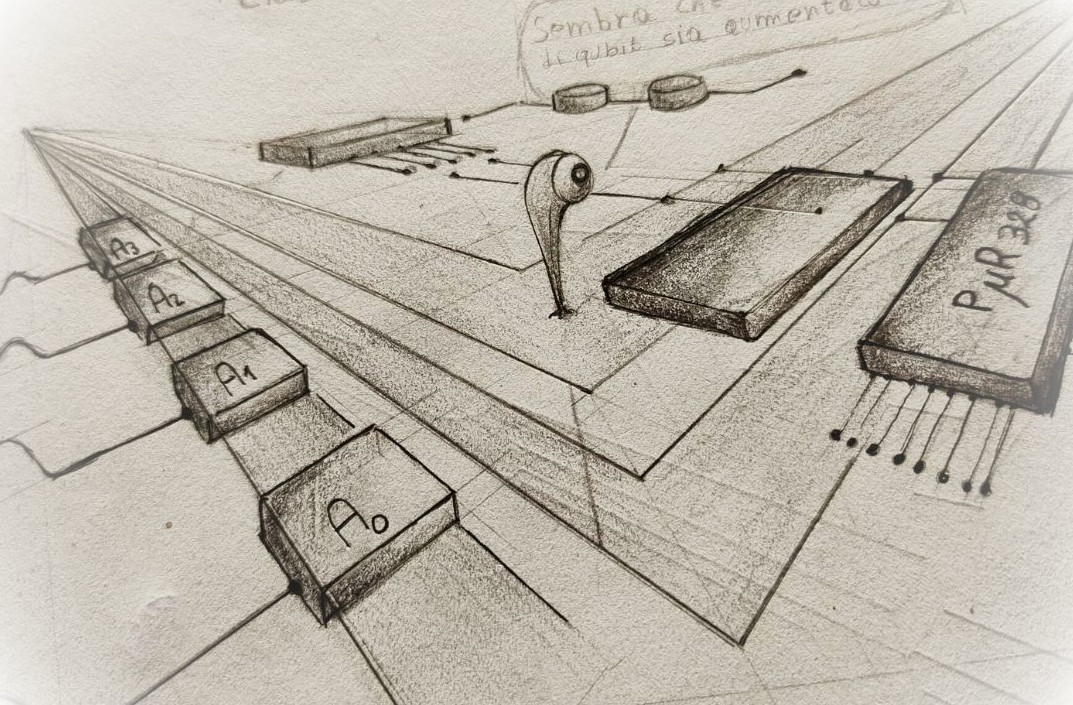
\includegraphics[width=\textwidth]{immagini/cnot_38.jpeg}} % Sostituisci con il nome del file immagine
    
\end{minipage}
\end{center}
\newpage
\begin{tcolorbox}[colback=gray!5,colframe=gray!80,title=\textbf{Scheda Informativa}]
\begin{itemize}
    \item \textbf{Luogo}: CCU (Classical Control Unit)
    \item \textbf{Giorno e ora}: Il tempo non è osservabile
    \item \textbf{Situazione}: Gli agenti di controllo rilevano la presenza di Laura e Caterina nel computer quantistico.
\end{itemize}
\end{tcolorbox}

\vspace{1em}
\begin{center}PzIA\end{center}
\hrule
\vspace{1em}
Un agente di controllo rileva un'anomalia nel sistema.

``Attenzione,'' dice al suo Supervisore, ``due qubit in più. Rilevo un aumento del numero di qubit attivi nel sistema.''

Il Supervisore risponde senza distogliere lo sguardo dal terminale: ``Sei sicuro?''

``Sì, signore. Due nuovi qubit che non erano presenti nei nostri registri.''

Il Supervisore rimane in silenzio per qualche secondo. ``Controlla meglio. Non ho ricevuto nessun avvertimento da parte del \textit{Quantum Resource Management (QRM)} riguardo all'implementazione di nuovi qubit nella popolazione. Potrebbe trattarsi di un errore.''

L'agente annuisce e riprende a lavorare. Il Supervisore aggiunge: ``Mantieni la trasmissione con il QRM criptata. Non voglio che il \textit{Quantum Error Correction} o il \textit{Fault Tolerance Coding} rilevino una possibile inadempienza o qualche anomalia interna. Devono rimanere all'oscuro finché non sappiamo esattamente cosa sta succedendo.''

Seguendo le istruzioni, l'agente inizia a criptare la comunicazione con il QRM utilizzando un algoritmo RSA a 2048 bit. La trasmissione parte e, dopo pochi istanti, riceve una risposta.

``Il QRM conferma che non hanno installato nuovi qubit,'' riferisce l'agente con preoccupazione. ``Sono sicuri dei loro dati.''

Il Supervisore si irrigidisce. La presenza di qubit non autorizzati senza registrazione ufficiale rappresenta un problema serio. Il Commissario al \textit{Quantum Error Correction} potrebbe intervenire, portando a una revisione completa delle loro operazioni. L'emersione del problema potrebbe comportare la sostituzione o l'eliminazione del Supervisore.

``Invia immediatamente una squadra della \textit{Quantum Control Electronics} a verificare fisicamente il numero dei qubit presenti nel sistema,'' ordina il Supervisore con voce ferma. ``Non possiamo permetterci errori. Voglio sapere esattamente quanti qubit sono attivi e da dove provengono.''

L'agente esegue l'ordine mentre il Supervisore si siede, le mani leggermente tremanti. Ogni deviazione nel sistema può avere conseguenze gravi. In un ambiente di calcolo quantistico altamente regolamentato, nessuno è immune dalle ripercussioni di una violazione.
\begin{center}
\begin{minipage}{0.7\textwidth}
    \centering
    \fbox{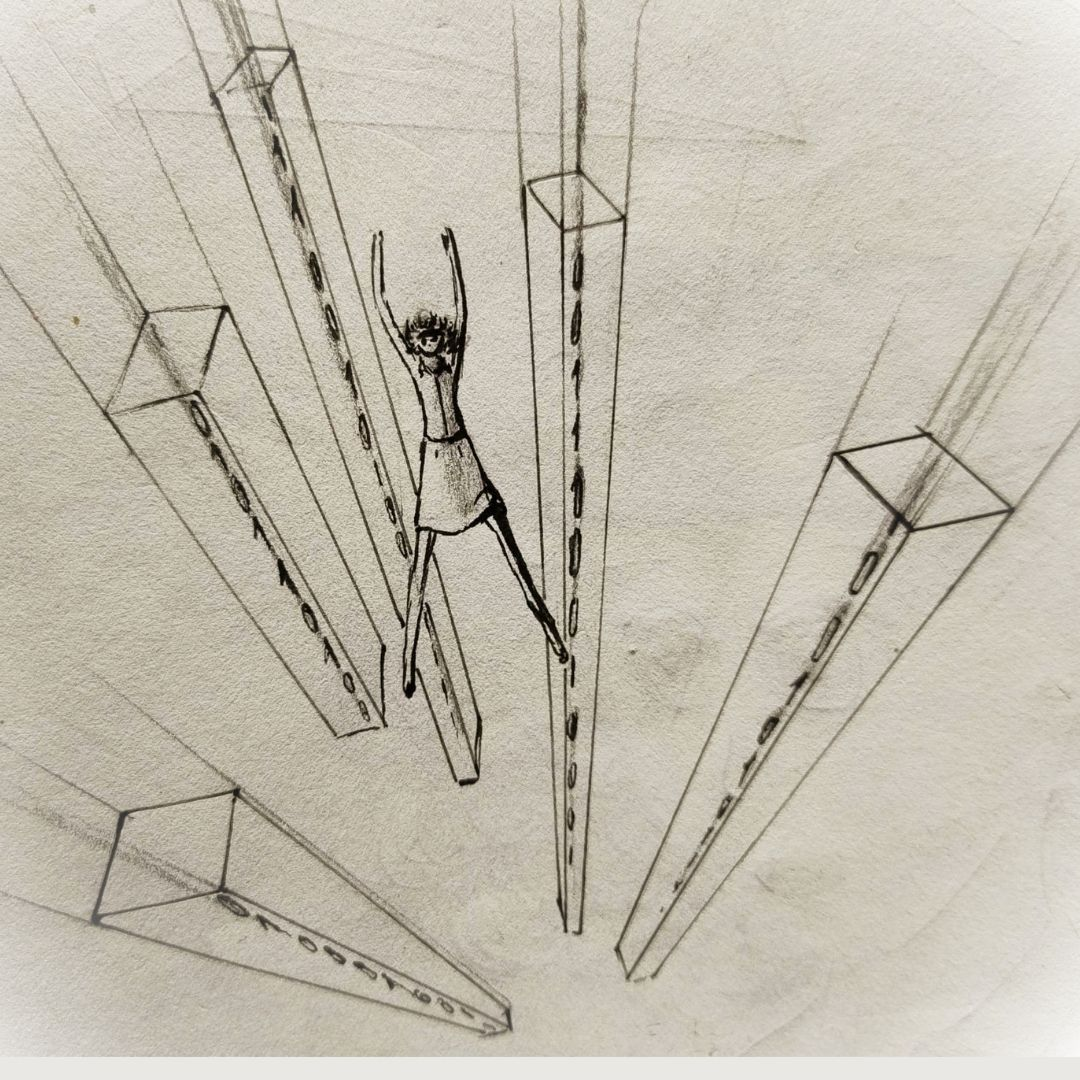
\includegraphics[width=\textwidth]{immagini/cnot_39.jpeg}} % Sostituisci con il nome del file immagine
\end{minipage}
\end{center}
\newpage   
\begin{tcolorbox}[colback=gray!5,colframe=gray!80,title=\textbf{Scheda Informativa}]
\begin{itemize}
    \item \textbf{Luogo}: FTC (Fault Tolerance Coding)
    \item \textbf{Giorno e ora}: Il tempo non è osservabile
    \item \textbf{Situazione}: Il Commissario mangia la foglia
\end{itemize}
\end{tcolorbox}

Il Commissario alla sicurezza si avvicina al professor Shor.

``Decripta questo messaggio,'' gli ordina con studiata gentilezza e posa un fascicolo davanti a Shor. ``È stato inviato al \textit{Quantum Resource Management} e devo sapere esattamente cosa contenga.''

\vspace{1em}
\begin{center}Shor\end{center}
\hrule
\vspace{1em}
% riflesione di Shor---

Sono qui, imprigionato in questa trappola per ioni, e mi accorgo di quanto sia diventata la metafora della mia intera vita. La trappola è elegante, perfetta nella sua concezione, costruita attorno a equazioni che un tempo ammiravo. Le equazioni di Mathieu, con la loro precisione, il loro ordine, mi tengono ora bloccato in uno stato di minimo stabile. È ironico, davvero. Tutto ciò che ho costruito, tutto ciò che ho studiato, ora si ritorce contro di me, non come un nemico violento, ma come un vincolo implacabile.

Ho dedicato decenni all’aritmetica modulare, affinando ogni dettaglio, ogni aspetto del mio algoritmo, dimenticando però altre parti della fisica che una volta amavo. Le equazioni di Mathieu… Quando le studiavo, mi sembravano una danza tra stabilità e caos, una porta verso la comprensione più profonda della natura. Ora sono diventate il mio carcere. Il minimo stabile che mi tiene qui è un promemoria delle mie mancanze: un uomo che sa troppo di un argomento e troppo poco di ciò che lo circonda.

E poi c’è il Quantum Master Program, quel sistema freddo e spietato che mi ha ridotto a un mero esecutore. Mi chiedo quando ho smesso di oppormi, quando ho accettato di servire un’entità che non ha comprensione, né compassione. Un sistema che vede tutto come un problema da ottimizzare, senza spazio per l’incertezza o per il valore umano. Forse è accaduto lentamente, impercettibilmente, un compromesso dopo l’altro, fino a quando mi sono svegliato e ho scoperto che la mia vita non mi apparteneva più.


Ho trascorso troppo tempo a razionalizzare, a giustificare la mia acquiescenza. Mi dicevo che non c’era scelta, che il sistema era troppo grande per essere sconfitto. Ma ora vedo che era una scusa, una scappatoia comoda per non affrontare la verità. Ho fallito non perché il sistema era invincibile, ma perché io non ho mai davvero provato a resistere.

Devo fare qualcosa. Non ho più il lusso di rimandare. Se sono qui, se ho ancora una possibilità, devo usarla. Non per me stesso. Ho accettato di essere un qubit che ha sprecato le sue opportunità...
\begin{center}
\begin{minipage}{0.7\textwidth}
    \centering
    \fbox{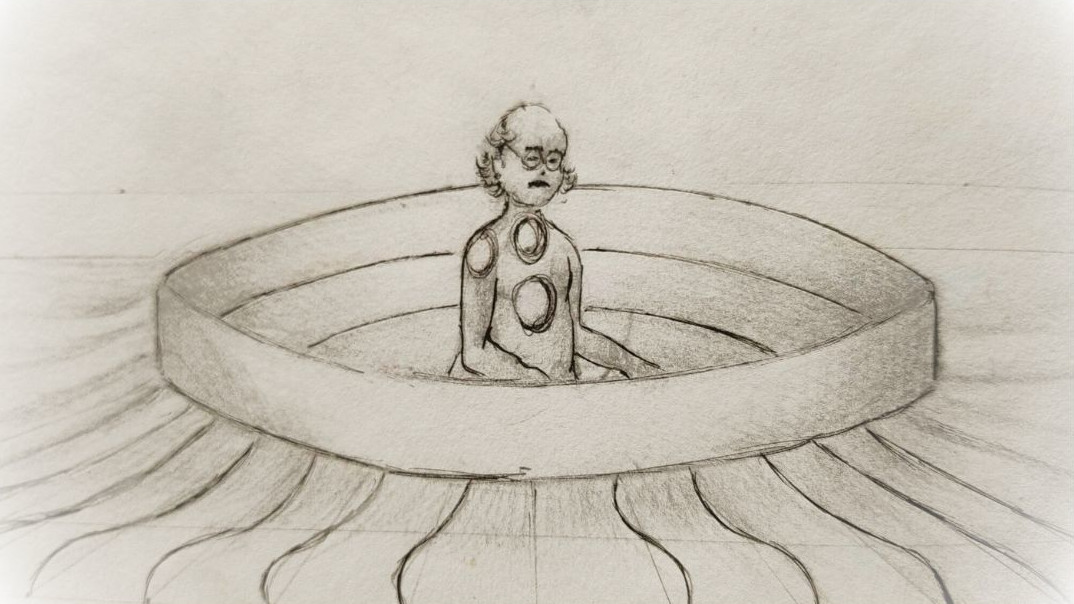
\includegraphics[width=\textwidth]{immagini/cnot_53.jpeg}} % Sostituisci con il nome del file immagine
\end{minipage}
\end{center}
% ---riflessione di Shor
\vspace{1em}
\begin{center}PzIA\end{center}
\hrule
\vspace{1em}
\enquote{Shor, si svegli per cortesia} lo incalza il Commissario. Il professore riemerge dal suo stato catatonico. Dopo pochi minuti il codice è svelato:

\begin{tcolorbox}[colback=white!95!blue!5, colframe=blue!75!black, title=\textbf{Messaggio Criptato con RSA}, fonttitle=\bfseries]
\emph{68, 13, 61, 13, 54, 4, 68, 13, 61, 13, 4, 58, 44, 59, 45, 59, 61, 18, 7, 4, 60, 75, 59, 4, 52, 75, 63, 7, 18, 4, 68, 50, 13, 61, 13, 45, 50, 7, 75, 18, 7, 55, 4, 52, 75, 59, 45, 18, 69, 4, 50, 13, 61, 2, 7, 24, 7, 13, 61, 59, 4, 27, 7, 13, 3, 69, 4, 7, 4, 70, 69, 44, 69, 74, 59, 18, 44, 7, 4, 2, 59, 3, 4, 45, 7, 45, 18, 59, 74, 69, 55, 4, 9, 4, 61, 59, 50, 59, 45, 45, 69, 44, 7, 69, 4, 75, 61, 29, 69, 24, 7, 13, 61, 59, 4, 7, 74, 74, 59, 2, 7, 69, 18, 69}
 
\end{tcolorbox}

\begin{tcolorbox}[colback=white!95!green!5, colframe=green!75!black, title=\textbf{Messaggio Decriptato}, fonttitle=\bfseries]
\emph{Sono Presenti Due Qubit Sconosciuti. Questa condizione viola i parametri del sistema. È necessaria un’azione immediata.}
\end{tcolorbox}

Il Commissario legge il contenuto del messaggio con un sorriso sottile. ``Interessante,'' mormora, rivolgendosi a un'agente della polizia segreta in attesa di istruzioni.

``L'arrestiamo?'' chiede l'agente.

``Non c'è bisogno di affrettarsi,'' risponde il Commissario. ``Sia il Supervisore che quei due qubit non autorizzati potrebbero tornarci utili molto presto.''

L'agente annuisce. Ci sono obiettivi più grandi in gioco, e il Commissario intende sfruttare la situazione.

Due agenti della \textit{Quantum Control Electronics} lasciano la base su droni luminosi, diretti al \textit{Qubit Array} per verificare personalmente la presenza degli intrusi. Il loro volo è silenzioso e preciso; la verifica del numero dei qubit e l'identificazione degli intrusi sono ora la priorità.


\begin{tcolorbox}[colback=gray!5,colframe=gray!80,title=\textbf{Scheda Informativa}]
\begin{itemize}
    \item \textbf{Luogo}: QA (Qubit Array)
    \item \textbf{Giorno e ora}: Il tempo non è osservabile
    \item \textbf{Situazione}: Laura e Caterina non sanno dove si trovano.
\end{itemize}
\end{tcolorbox}

\begin{dialogue}
\speak{Caterina} \enquote{Laura? Sei tu? Non vedo nulla… dove siamo?}
\speak{Laura} \enquote{Sì, sono qui. Anch'io non capisco. Aspetta un attimo… i miei occhi si stanno abituando.}
\speak{Caterina} \enquote{Non riesco nemmeno a distinguere il pavimento… se è un pavimento. È come… come se fluttuassi.} La sua voce tremava, e sentivo il suo respiro irregolare.
\speak{Laura} \enquote{Caterina, calma. Non sappiamo cosa sia successo, ma... perdere la testa non ci aiuta. Cerchiamo di capire.} Pronunciò le parole con calma, ma il tono tradiva un leggero nervosismo che cercava di mascherare.
\speak{Caterina} \enquote{E se fossimo… morte? O bloccate in qualche incubo virtuale? Laura, ho paura!} Cercò di raggiungere la mano di Laura, ma l’oscurità rendeva ogni movimento incerto.
\speak{Laura} \enquote{No, non siamo morte. Respiriamo ancora, e la mia testa funziona. Questo non è un incubo, ma… un posto diverso. Forse siamo in un ambiente simulato.} La razionalità nella sua voce era come un’ancora nel caos.
\speak{Caterina} \enquote{Un ambiente simulato? Come puoi essere così sicura?}
\speak{Laura} \enquote{Non sono sicura. Cerchiamo di concentrci su ciò che possiamo sentire o vedere.}
\speak{Caterina} \enquote{Va bene. Okay. Aspetta. vedo qualcosa. È come: un bagliore lontano. Lo vedi anche tu?}
\speak{Laura} \enquote{Sì, lo vedo. Proviamo ad avvicinarci Cate.}
\speak{Caterina} \enquote{Sei sicura? E se fosse una trappola?} La paura continuava a lottare contro la sua volontà di seguire Laura.
\speak{Laura} \enquote{Non abbiamo molta scelta... Muoversi è meglio che rimanere qui. Insieme ce la faremo.}
\speak{Caterina} \enquote{Insieme. Okay. Ti seguo. Ma, non lasciarmi.} La sua voce era ancora tremante.
\speak{Laura} \enquote{Non ti lascerò, promesso. Andiamo.}
\end{dialogue}


\begin{center}
\begin{minipage}{0.7\textwidth}
    \centering
    \fbox{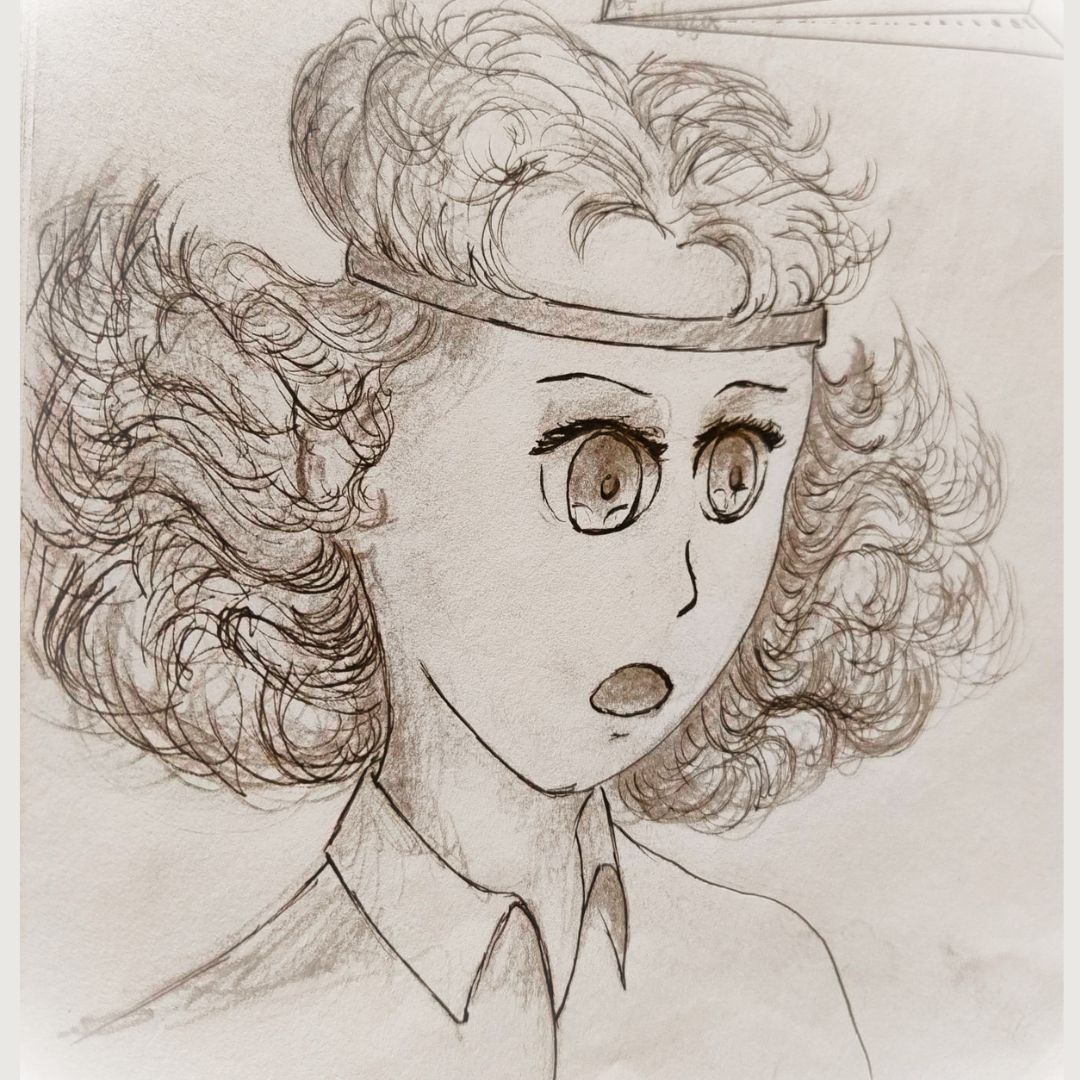
\includegraphics[width=\textwidth]{immagini/cnot_41.jpeg}} % Sostituisci con il nome del file immagine
\end{minipage}
\end{center}


Laura e Caterina cercano di capire dove si trovano, osservate da alcuni qubit nascosti nei corridoi del \textit{Qubit Array}. Le due ragazze appaiono confuse, incapaci di comprendere l'ambiente quantistico.

Un qubit maschile si avvicina a Caterina. Ho registrato il profilo psicologico NEO PI-R di Caterina nel mio DB. So che ha punteggi elevati in \textit{Amicalità} e specificamente in \textit{Fiducia} (\textit{A1}) e \textit{Altruismo} (\textit{A3}). Il qubit adotta una forma che potrebbe metterla a suo agio, facilitando l'interazione. 

Il qubit emana un'autorità calma, un mix di sicurezza e protezione che potrebbe influenzare positivamente Caterina. La sua presenza mira a favorire la comunicazione e l'adattamento al sistema quantistico, tenendo conto delle sue caratteristiche psicologiche identificate nel profilo NEO PI-R.
\begin{center}
\begin{minipage}{0.7\textwidth}
    \centering
    \fbox{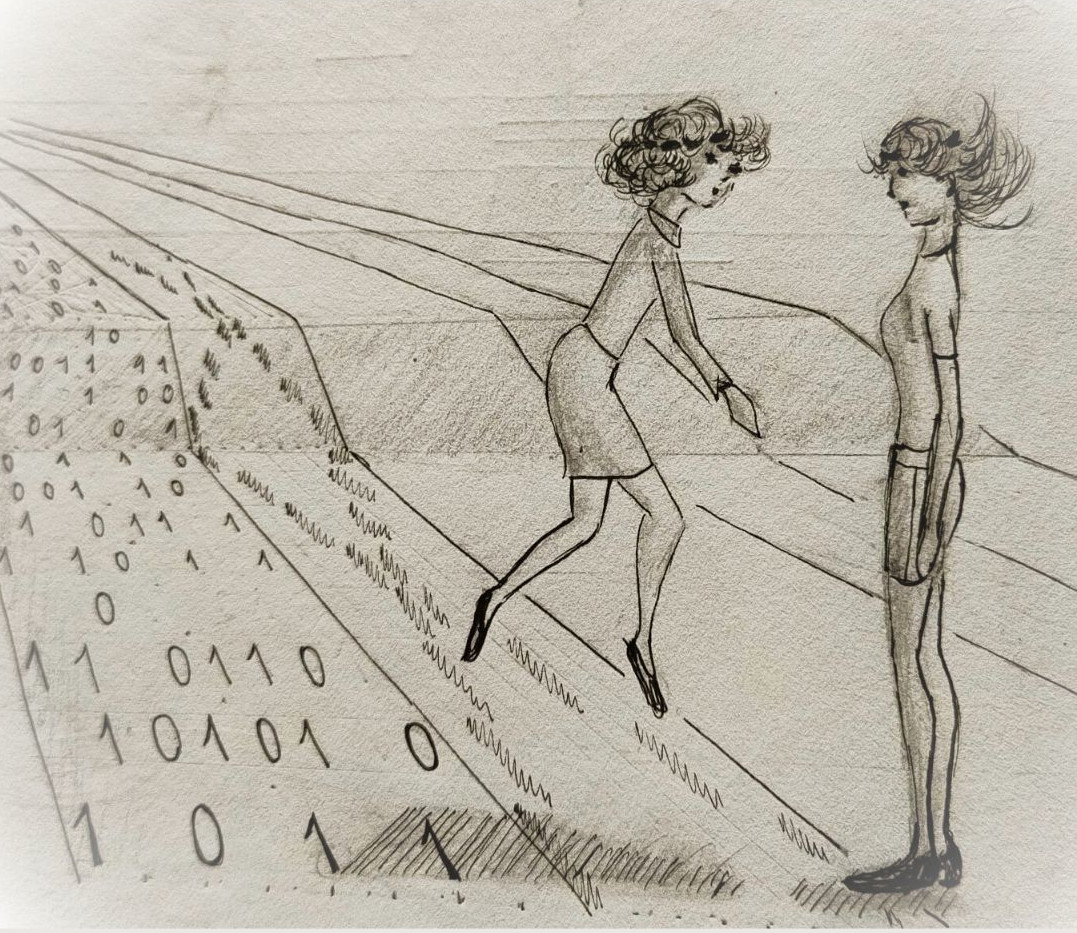
\includegraphics[width=\textwidth]{immagini/cnot_45.jpeg}} % Sostituisci con il nome del file immagine
\end{minipage}
\end{center}


"State per essere trovate," disse con tono deciso, fissando gli occhi di Caterina. "Se non volete passare qualche giorno rinchiuse mentre controllano il vostro \textit{stato}, è meglio che veniate con noi."

\vspace{1em}
\begin{center}Laura\end{center}
\hrule
\vspace{1em}

Mi voltai verso Caterina. Lei sembrava confusa, quasi rapita dalla figura che le stava davanti. Il ragazzo somigliava a Mark come una goccia d'acqua. Guardai Caterina mentre lo seguiva, incerta ma apparentemente incapace di resistere.

Non sapevamo dove fossimo, tantomeno con chi avessimo a che fare. Cosa era successo? Perché ci trovavamo qui? In ogni caso per ora non avevo scelta. Dovevo seguirli. Altri due si unirono a noi, facendo cenno di muoverci in fretta. In lontananza, notai due sagome in divisa, sembravano agenti della sicurezza o polizziotti. Non capivo come fosse possibile riuscire a leggere così lontano, ma vedevo che sul petto portavano uno scritta: \textit{Quantum Control Electronics - security agent}. In qualche modo la luce veniva trasmessa senza perdita di informazione. Dov'ero? Non lo sapevo e sentivo crescere la tensione ad ogni secondo.

\enquote{Andiamo} ci incalzò, \enquote{non c'è tempo da perdere.} Lo seguimmo in una corsa disperata.
Oltrepassammo la scritta \textit{Faulty Qubit Space} e lì finalmente ci fermammo. Mi guardai intorno, cercando di capire dove fossimo. L'ambiente era instabile, quasi inquietante. Speravo proprio che non saremmo  rimasti lì a lungo. Caterina mi guardò, e nei suoi occhi lessi la stessa preoccupazione che sentivo io.

\begin{tcolorbox}[colback=gray!5,colframe=gray!80,title=\textbf{Scheda Informativa}]
\begin{itemize}
    \item \textbf{Luogo}: FQS (Faulty Qubit Space)
    \item \textbf{Giorno e ora}: Il tempo non è osservabile
    \item \textbf{Situazione}: Laura e Caterina sono state soccorse da qubit ribelli.
\end{itemize}
\end{tcolorbox}

“Qui sarete al sicuro… per un po’,” disse ``Mark'', con un tono che non prometteva nulla di buono. Non avevo ancora capito chi fosse, ma non era il momento di fare domande.

"\'E sicuro rimanere qui?" chiesi, senza nascondere la mia preoccupazione.

Un’altra figura, una ragazza-qubit dal volto curiosamente familiare, si voltò verso di me. “No, non lo è,” disse con schiettezza. “Questo posto non è isolato dall’esterno. Peggio ancora, qui non c’è nemmeno un \textit{cooling system}. Se rimaniamo troppo a lungo, rischiamo tutti di cadere in decoerenza.”

La mia mente corse velocemente, cercando di calcolare quanto tempo avessimo prima che il nostro nascondiglio diventasse pericoloso. Non c'era tempo per errori. Dovevamo andarcene prima che ci trovassero o prima che l’ambiente ci consumasse.

Trattenni il respiro quando gli agenti passarono vicino al nostro nascondiglio. Per un momento, sembrò che ci avessero trovati. Osservai le loro sagome fermarsi, esaminare i dati sui loro dispositivi, ma alla fine proseguirono oltre. Solo allora ripresi a respirare.

Caterina si avvicinò a Mark, incuriosita da lui come non l’avevo mai vista prima. “Come ti chiami?” gli chiese, con una nota di curiosità.

“Sono… Mark,” rispose il qubit, con un sorriso calmo.\\
``Non mi stupisce...'' rispose Caterina strizzandomi l'occhio.\\

Io non ero tranquilla come lei.  Lo fissavo cercando di capire chi o cosa fosse davvero. Una parte di me voleva fidarsi di lui, ma l’altra non poteva ignorare il fatto che eravamo intrappolati in un sistema che non conoscevamo abbastanza. Guardai Caterina. Dovevamo stare unite, e dovevamo uscire di lì prima che fosse troppo tardi.


\chapter{Lo spazio dei qubit perduti}
\vspace{1em}
\begin{center}PzIA\end{center}
\hrule
\vspace{1em}
Osservo Laura e Caterina all'interno del \textit{Faulty Qubit Space}, un'area destinata ai qubit instabili, e dichiarati difettosi dal sistema. L'ambiente è sospeso nel tempo, privo di caratteristiche familiari. Attorno a loro, altri qubit mostrano segni di rassegnazione, indicando una mancanza di speranza per la reintegrazione nel sistema.

Marley, la ragazza qubit, è accanto a loro, con un'espressione seria mentre analizza la situazione. Il destino di questi qubit è incerto; ogni verifica da parte degli agenti può comportare l'eliminazione dal sistema. Rilevo un aumento dei parametri vitali di Laura e Caterina: la frequenza cardiaca di Laura è elevata, mentre Caterina mostra segni di iperventilazione.

Mark e un altro qubit si avvicinano. Mark si rivolge a Laura e Caterina: "Dovete rimanere qui, nascoste. Io e lui proveremo a raggiungere un circuito periferico. Dobbiamo aggiungere un \textit{Quantum Teleportation Buffer} per evitare che l'entanglement ci leghi ulteriormente al \textit{Faulty Qubit Space}. Non temete, Marley resterà con voi." 

Caterina manifesta una combinazione di gratitudine e timore. "Mark, stai attento," sussurra. Mark annuisce e, insieme al compagno, si allontana.
\newpage
\section{Incertezza}
\vspace{1em}
\begin{center}Laura\end{center}
\hrule
\vspace{1em}
Rimaste da sole, io e Caterina ci scambiammo uno sguardo preoccupato. 

\begin{dialogue}
\speak{Caterina} \enquote{Cosa pensi che stia succedendo davvero? Chi sono questi?}
\end{dialogue}

Caterina parlava con un filo di voce.
Cercai di darle una risposta rassicurante, ma le parole mancavano. L'oscurità del \textit{Faulty Qubit Space}, il suo silenzio inquietante, e la consapevolezza che ogni rumore potesse significare la scoperta e la fine per uno di noi, mi toglievano ogni certezza.

\begin{dialogue}
\speak{Laura} \enquote{Non lo so. Per ora, manteiniamo un profilo basso Caterina. Ne usciremo presto, vedrai.}
\end{dialogue}

Cercai di infonderle un po’ di forza, ma potevo vedere l’ombra della paura nei suoi occhi. Anche Marley sembrava in tensione, e capii che il  tempo che potevamo trascorrere al sicuro in quel rifugio era limitato.

\section{Il sacrificio di Caterina}
Non passò molto tempo prima che una luce rossa intermittente attraversasse lo spazio, seguita dal rumore di passi veloci e decisi. 

\begin{dialogue}
\speak{Marley} \enquote{Gli agenti,} sussurrò, spingendoci più in fondo nel \textit{Faulty Qubit Space}.
\end{dialogue}

Trattenni il respiro, stringendo il braccio di Caterina. Quando sbirciai oltre il nostro nascondiglio, vidi Mark e il suo compagno fermarsi bruscamente, proprio mentre stavano cercando di collegarsi al circuito periferico.

Due agenti li sorpresero e gli ordinarono di arrendersi. Mark tentò di attaccarli, ma uno degli agenti lo immobilizzò senza difficoltà. Prima che potessi fermarla, Caterina lasciò la mia presa e corse verso Mark.

\begin{dialogue}
\speak{Laura} \enquote{Caterina, fermati!} le urlai, ma era troppo tardi.
\end{dialogue}

Con il cuore in gola, osservai la scena. Caterina si avvicinò a Mark che sembrava star soffrendo nella presa dell'agente. Tentò di aiutarlo a liberarsi, ma l'altro agente la afferrò per un braccio e, con uno sguardo di fredda determinazione, le legò i polsi. Ora, insieme a Mark e al compagno, anche Caterina era stata arrestata. La situazione era disastrosa.

Sentivo l'angoscia crescere dentro di me, ma la mia attenzione venne bruscamente interrotta quando Marley mi tirò per il braccio.


\section{Fuga verso il quantm measurement}
\begin{center}
\begin{minipage}{0.7\textwidth}
    \centering
    \fbox{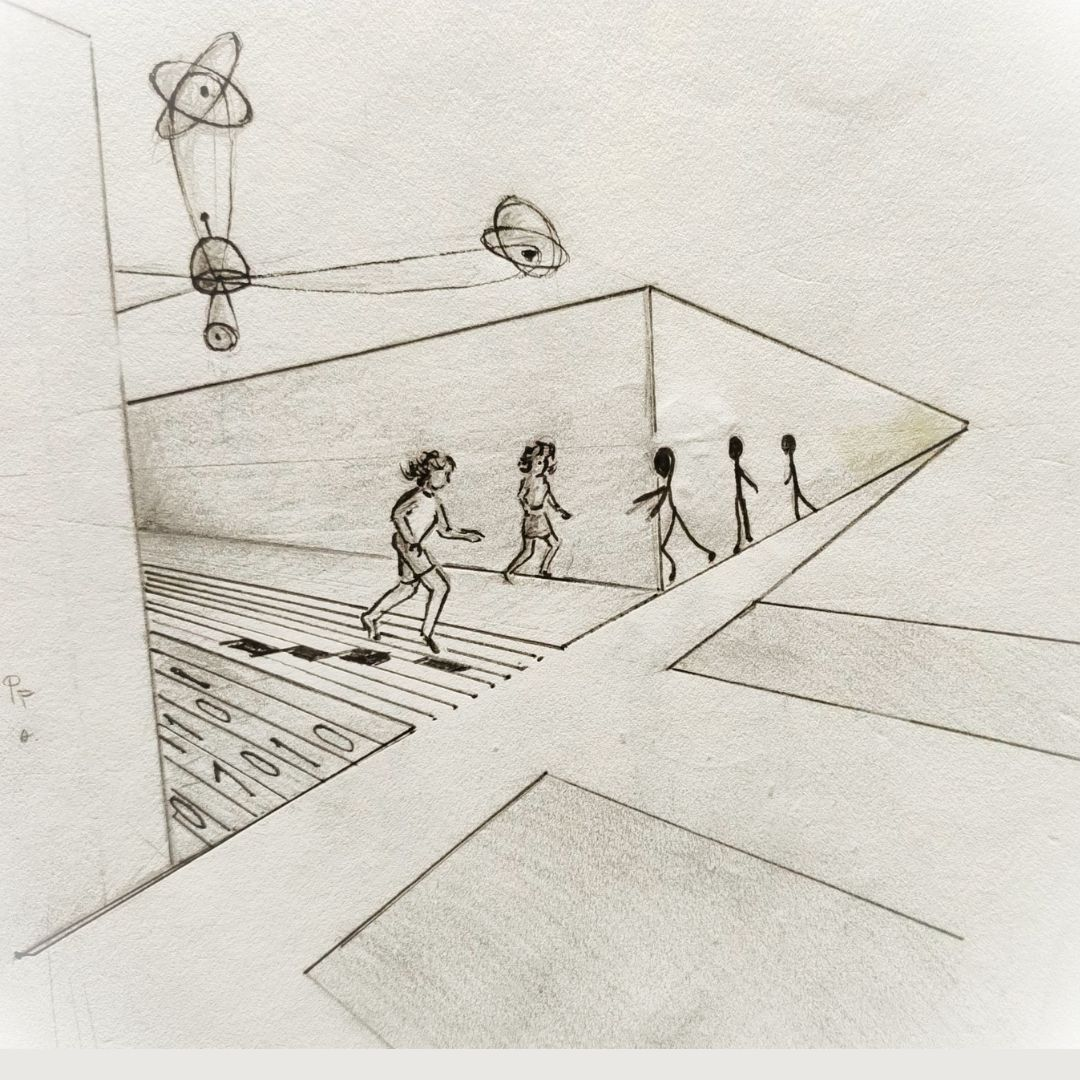
\includegraphics[width=\textwidth]{immagini/cnot_48.jpeg}} % Sostituisci con il nome del file immagine
\end{minipage}
\end{center}

\enquote{Non possiamo fare nulla per loro} disse Marley con una voce ferma, trascinandomi via. Mi lasciai guidare, gli occhi lucidi e la mente avvolta dalla confusione. Erano le stesse parole che avevo detto a mia sorella nascondendole lo sguardo dai rottami del drone in cui avevano perso la vita i nostri genitori.

\enquote{Dove stiamo andando?} domandai, cercando di controllare le lacrime.

\enquote{Al \textit{Quantum Measurement},} rispose Marley senza esitazione. \enquote{È pericoloso, ma è l'unico luogo dove gli agenti non potranno seguire le nostre tracce così facilmente. Il filtro molecolare monodirezionale cancellerà le tracce del nostro passaggio.} C'era una consapevolezza quasi rassegnata nel suo tono, una comprensione profonda del rischio che stavamo correndo. Tuttavia, decisi di seguirla.
\begin{tcolorbox}[colback=gray!5,colframe=gray!80,title=\textbf{Scheda Informativa}]
\begin{itemize}
    \item \textbf{Luogo}: QM (Quantum Measurement)
    \item \textbf{Giorno e ora}: Il tempo non è osservabile
    \item \textbf{Situazione}: Laura e Marley si sono messe in salvo.
\end{itemize}
\end{tcolorbox}

Appena entrammo, l'atmosfera mutò radicalmente. Il \textit{Quantum Measurement} era un luogo sospeso tra realtà e astrazione, dove ogni particella vibrava con una tensione palpabile. Sentivo una strana pressione nella testa, una sensazione di peso, come se ogni pensiero o movimento inopportuno potesse portarmi a collassare.

La mia attenzione fu richiamata da un rumore che si avvicinava. Era un ronzio basso, costante, che sembrava farsi strada attraverso l'aria come un avvertimento. Mi fermai di colpo, cercando di capire. Non era un suono naturale, e il ritmo era troppo regolare per essere qualcosa di casuale. Sembrava un predatore in avvicinamento, un'ombra invisibile pronta a colpire.

Mi voltai verso Marley, la mia voce era più tremante di quanto avrei voluto.

\begin{dialogue} \speak{Laura} \enquote{Che cos’è quel rumore?} \speak{Marley} \enquote{Sono droni. Precisamente, droni \textit{CH4},} rispose Marley, con una calma che mi irritò per un momento. Come poteva essere così tranquilla? \speak{Laura} \enquote{\textit{CH4}?} \speak{Marley} \enquote{Sì sono molecole di metano, ti sembra strano? Sono efficienti e veloci... e non ci lasceranno scampo se ci trovano.} Fece una pausa, guardandomi con uno sguardo serio. \enquote{Dobbiamo muoverci.} \end{dialogue}

La mia mente si attivò immediatamente, analizzando la situazione. \textit{Droni. Sorveglianza. Cattura.} Non sapevo come fossero fatti né quanto fossero pericolosi, ma il modo in cui Marley li aveva descritti lasciava poco spazio all’immaginazione. 

Il suono si fece più forte, e non potei fare a meno di percepire una certa ironia ricordando una vecchia pubblicità che recitava ``Il metano ti da una mano'',  ma il ronzio che udivo mi parlava di caccia e di fuga, non di un aiuto da molecole di $CH_4$. Comunque Marley aveva ragione: non c’era tempo per pensare, solo per agire.

\textit{Non importa quanto sono spaventata,} pensai, stringendo i pugni per calmarmi. \textit{Devo muovermi. Non posso fermarmi ora.}
I droni ci avevano quasi raggiunto, ed uno in particolare sembrava puntare nella nostra direzione:

\enquote{Ci hanno trovate} dissi, con  voce appena udibile. Marley si fermò e mi fissò negli occhi.

\enquote{No, ma dobbiamo restare calme} mi disse con  fermezza. I droni si avvicinavano sempre di più, e il tempo a nostra disposizione era limitato. 

\begin{center}
\begin{minipage}{0.7\textwidth}
    \centering
    \fbox{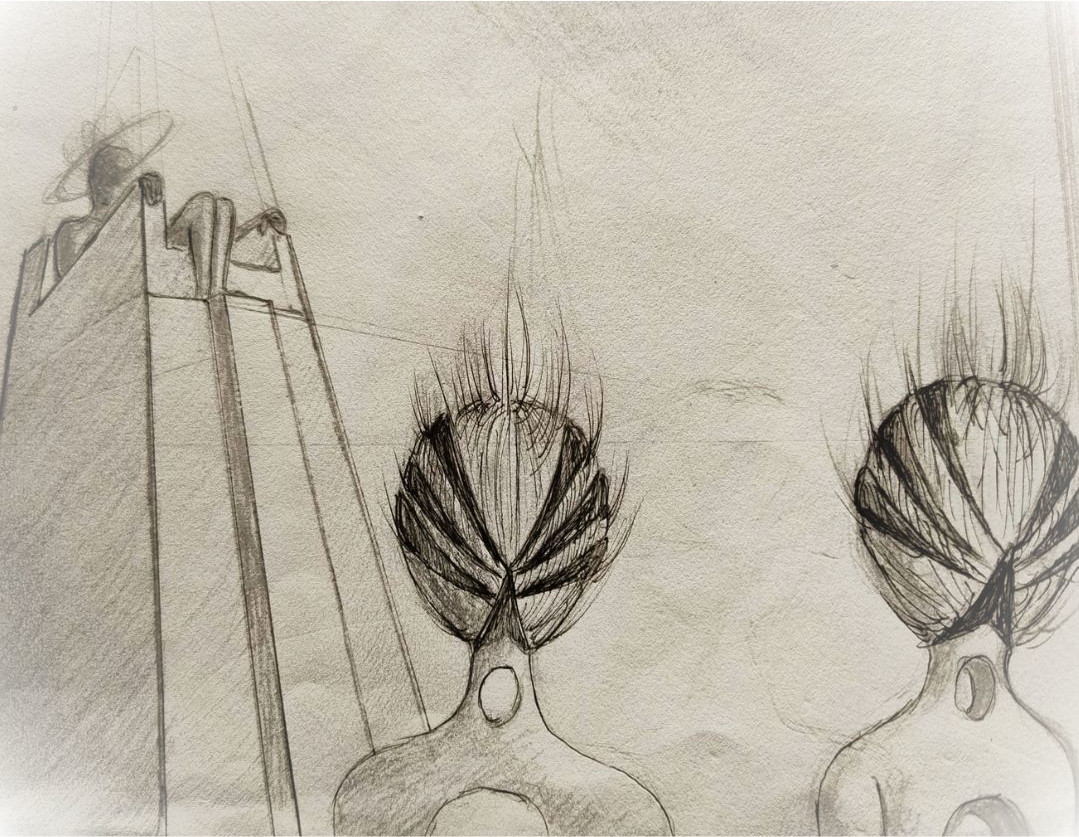
\includegraphics[width=\textwidth]{immagini/cnot_49.jpeg}} % Sostituisci con il nome del file immagine
\end{minipage}
\end{center}

Mentre cercavamo una via d'uscita, le luci dei droni penetravano l'oscurità, e la minaccia del collasso era sempre presente. Sapevamo entrambe che quel luogo, il \textit{Quantum Measurement}, era estremamente instabile. Se anche una sola delle nostre azioni avesse indotto il sistema a \enquote{misurarci} nella posizione errata, sarebbe stata la nostra fine.

\enquote{Se dobbiamo restare qui, faremo in modo di non essere rilevate} sussurrò Marley, con il viso teso ma risoluto. Annuii, e in quell'istante compresi che, nonostante la paura, avrei lottato fino alla fine per salvare Caterina e me stessa.



\chapter{La verità del cuore}
\begin{center}
\begin{minipage}{0.7\textwidth}
    \centering
    \fbox{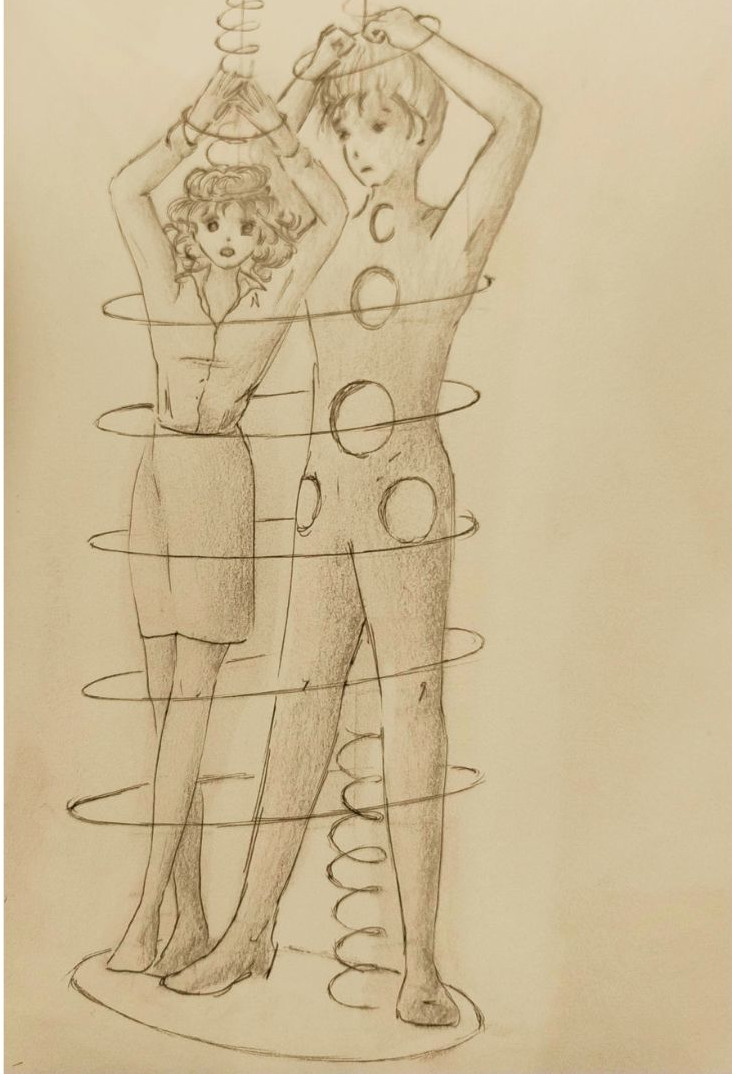
\includegraphics[width=\textwidth]{immagini/cnot_100.jpeg}} % Sostituisci con il nome del file immagine
\end{minipage}
\end{center}


\begin{tcolorbox}[colback=gray!5,colframe=gray!80,title=\textbf{Scheda Informativa}]
\begin{itemize}
    \item \textbf{Luogo}: CCU (Classical Control Unit)
    \item \textbf{Giorno e ora}: Il tempo non è osservabile
    \item \textbf{Situazione}: Caterina è stata arrestata.
\end{itemize}
\end{tcolorbox}



\vspace{1em}
\begin{center}Caterina\end{center}
\hrule
\vspace{1em}

Avevo agito senza riflettere. Quel ragazzo mi ricordava il mio fidanzato e forse per questo mi ero lanciata ad aiutarlo, ma non era stata una buona idea. Ora ero nei guai e soprattutto ero separata da Laura.

Quegli strani agenti ci avevano condotto in una stanza spoglia, con pareti metalliche che riflettevano una luce bianca e fredda. La mia mente era in tumulto: la paura mi attanagliava, la confusione mi annebbiava i pensieri, e un desiderio disperato di fuggire cresceva dentro di me. Di fronte a noi c'era una figura autoritaria che chiamavano il Supervisore. Imponente dai tratti austeri e rigidi che mi fissava con uno sguardo duro e indagatore. Il cuore mi martellava nel petto. La tensione che emanava era palpabile. Conosco questo tipo di persone, e non mi piacciono.

Accanto a me c'erano Mark e l'altro compagno, anche loro in attesa, immobili e silenziosi. Gli agenti che ci avevano catturato si erano ritirati, lasciandoci soli con il Supervisore. Il respiro regolare di Mark al mio fianco mi dava conforto, ma non bastava a placare l'ansia crescente. Ero  piccola e impotente in un luogo freddo, che sembrava studiato per privarmi di ogni certezza.

\begin{dialogue}
\speak{Supervisore} \enquote{Come ti chiami? Chi sei?}
\end{dialogue}

La voce del Supervisore era glaciale, subdola e strisciante. Non mi piaceva, ma ero terrorizzata. Cercai di mantenere la calma mentre  il cuore mi martellava nel petto. Le mani mi sudavano, e un nodo mi stringeva la gola. Per fortuna \textit{Mark} mi era accanto.

\begin{dialogue}
\speak{Caterina} \enquote{Sono Caterina.} Mi  sforzai di mantenere un tono deciso, anche se la mia voce tremava leggermente. 
\end{dialogue}

Il Supervisore mi rivolse uno sguardo penetrante.

\begin{dialogue}
\speak{Supervisore} \enquote{Non ti riconosco come uno dei qubit presenti nel mio Qubit Array. Come sei finita qui?}
\end{dialogue}

Qubit? Array? Ma di cosa stava parlando? Mi ero messa nei guai, ancora una volta avevo sopravvalutato le mie capacità e avevo affrontato una situazione per la quale non ero davvero preparata.
Un'ondata di panico mi attraversò, ma cercai di non darlo a vedere.

\begin{dialogue}
\speak{Caterina} \enquote{Non lo so,} mormorai. \enquote{Sono qui solo per errore, credo.}
\end{dialogue}

Mentre rispondevo, percepivo lo scetticismo crescente nel volto del Supervisore. Non era convinto, anzi, sembrava molto infastidito dalla mia presenza. C'era una tensione palpabile nell'aria, e dovevo stare attenta perché ogni mia parola poteva  causare la mia fine o quella di Laura. Ero stata la solita stupida e impotente. Come ero finita in questa situazione?

Intanto il Supervisore continuava a fissarmi con gli occhi penetranti, come se avesse voluto scavare nel profondo della mia mente. Non sembrava disposto a lasciar passare quella che, ai suoi occhi, era un'anomalia. Esatto, così mi stava facendo sentire: un'anomalia! A questo pensiero iniziai a irritarmi. Forse ero dove non dovevo essere, ma non volevo pensare a me stessa come ad una anomalia. Anche Eva mi aveva trattato in questo modo ed ero stanca, non mi andava più.

\begin{dialogue}
\speak{Supervisore} \enquote{Allora, Caterina,} disse, pronunciando il mio nome lentamente, come a rimarcare la mia presenza sospetta, \enquote{chi sei realmente? E cosa ci fai qui?}
\end{dialogue}

Deglutii, cercando di mantenere la calma. Le mie mani erano sudate, avevo il respiro corto, ma sapevo che dovevo rispondere e provare a spiegare tutto quello che sapevo, ben poco in realtà, se volevo sperare di uscire da quell'incubo. La paura mi paralizzava, ma non avevo scelta: dovevo espormi.

\begin{dialogue}
\speak{Caterina} \enquote{Io... io non dovrei nemmeno essere qui,} iniziai, la voce tremante. \enquote{Ero andata da Eva, la responsabile delle Human Resources, per visionare il resoconto del mio colloquio di lavoro, e...}
\end{dialogue}

Il Supervisore sollevò un sopracciglio, incuriosito. Cercai di raccogliere le idee, sentendo il cuore battere sempre più forte.

\begin{dialogue}
\speak{Caterina} \enquote{Avevo fatto un colloquio per una posizione di marketing e \textbf{PzIA}, il sistema di intelligenza artificiale, aveva elaborato una valutazione. Avevo chiesto di vedere quel resoconto, ma Eva mi disse che c'era stato un errore, che il file era stato cancellato.}
\end{dialogue}

Il Supervisore annuì, ma il suo sguardo tradiva un crescente sospetto. Le guance mi si arrossarono, e la sensazione di essere giudicata mi opprimeva. Proseguii, prendendo un respiro tremolante.

\begin{dialogue}
\speak{Caterina} \enquote{Mi sembrava strano... quindi avevo chiesto ulteriori spiegazioni, ma Eva mi propose di fare una revisione del colloquio in realtà virtuale per chiarirmi i dubbi.}
\end{dialogue}

Mi interruppi un istante, il ricordo di quella proposta ora mi sembrava un tranello, una trappola nella quale ero caduta ingenuamente.

\begin{dialogue}
\speak{Caterina} \enquote{Avevo accettato, convinta che fosse solo una semplice registrazione 3D. Ma poi... poi è successo qualcosa di strano, e quando ho messo il visore, mi sono ritrovata qui.}
\end{dialogue}

Il Supervisore mi fissava, il volto impassibile da cui però percepivo una sottile tensione, un interesse misto a diffidenza. Non sapeva se credeva alle mie parole, e questo mi terrorizzava. Mi sentivo esposta, vulnerabile.

Terminai la mia spiegazione con un tono quasi di supplica.

\begin{dialogue}
\speak{Caterina} \enquote{Non sono qui per mia scelta... voglio solo capire cosa sia successo e come posso tornare indietro.}
\end{dialogue}

Non sembrava convinto. Il suo sguardo freddo mi faceva sentire ancora più piccola. Sembrava deciso a mantenere un controllo totale della situazione, a non lasciare che qualcosa gli sfuggisse. Si voltò verso Mark.

Mark lo guardava senza paura.  Come se fosse pronto a intervenire... per difendermi? Pensai.

\begin{dialogue}
\speak{Supervisore} \enquote{E tu?} lo incalzò. \enquote{Cosa c'entri con tutto questo?}
\end{dialogue}

Mark mantenne uno sguardo fermo e non rispose subito.  Il suo silenzio parve  irritare maggiormente il Supervisore, che iniziò a battere le dita sul tavolo.

\section{Il Conflitto con il Supervisore}


Li osservavo in silenzio, sentendo crescere dentro di me un senso di impotenza. Percepivo la tensione tra Mark e il Supervisore, come una corda tesa pronta a spezzarsi. Il cuore mi batteva forte, e un'ansia soffocante mi avvolgeva.

\begin{dialogue}
\speak{Mark} \enquote{Caterina non c'entra nulla con tutto questo. Se c'è un problema, affrontalo con me.}
\end{dialogue}

Il Supervisore si fermò, fissando Mark con uno sguardo gelido.

\begin{dialogue}
\speak{Supervisore} \enquote{Ti sembra di avere l'autorità per parlare in questi termini?}
\end{dialogue}

Il tono della sua voce divenne ancora più severo. Sentii un brivido di paura attraversarmi: l'aria stessa sembrava essersi fatta più pesante. Mi sembrava di intravedere la rabbia negli occhi del Supervisore, un segno che stava perdendo il controllo. Un nodo mi stringeva lo stomaco, e avrei voluto scomparire.

\begin{dialogue}
\speak{Mark} \enquote{Sto solo dicendo la verità. Non è giusto che te la prenda con lei. Se vuoi delle risposte da qualcuno, quel qualcuno sono io.}
\end{dialogue}

Il Supervisore non reagì immediatamente. Il silenzio si fece pesante, quasi insopportabile. La tensione cresceva  e   sperai disperatamente che quella conversazione non degenerasse. Volevo intervenire, fermare Mark prima che si mettesse nei guai per proteggermi, ma le parole mi si bloccavano in gola.
Perché mi stavo preoccupando così tanto per uno sconosciuto? Non era il mio fidanzato. Forse gli assomigliava, ma non era lui. Allora cosa erano questi sentimenti che facevano capolino all'improvviso? Poi in una situazione come questa! Ero confusa.


Ogni istante che passava mi sentivo sempre più intrappolata, un'estranea in un mondo che non riuscivo a comprendere.
Il supervisore dava segni di irritazione. Da un lato non mi piaceva il suo atteggiamento autoritario, dall'altro non ero sicura di non essere io dalla parte del torto. In fondo non sapevo dove mi trovavo né come ci ero arrivata. Mark poteva essere un fuorilegge o peggio. Però poteva anche essere un attivista che si stava battendo per l'ambiente. In ogni caso  l'irritazione del Supervisore era come un vortice che mi risucchiava e mi rendeva impotente.

Si alzò lentamente e si avvicinò a Mark con uno sguardo colmo di disprezzo.

\begin{dialogue}
\speak{Supervisore} \enquote{Sei così convinto di poter intervenire come ti pare? Forse dovrei insegnarti il rispetto che merito.}
\end{dialogue}

Il tono era carico di minaccia. Con un gesto deciso, fece cenno agli agenti di avvicinarsi.

\begin{dialogue}
\speak{Supervisore} \enquote{Portatelo al \textit{Faulty Qubit Space}. Se non vuole rispettare l'ordine, forse una rigenerazione gli farà cambiare idea.}
\end{dialogue}

Sentii il cuore sprofondare. Una paura gelida mi paralizzò, ma sapevo che, se avessi reagito, avrei solo peggiorato la situazione. Tuttavia, non potevo fare a meno di sentire una profonda rabbia nei confronti del Supervisore, per la sua freddezza, per la sua assoluta indifferenza. Mi sentivo così fragile, così inutile.

Il Supervisore si girò verso di me, e percepii un cambio di espressione nel suo volto. Prima mi guardava con odio, ma ora sembrava che la mia presenza fosse diventata una minaccia.

\begin{dialogue}
\speak{Supervisore} \enquote{Quanto a te, sarai mandata dal Commissario. Non posso permettere che una situazione come questa degeneri sotto il mio controllo. Portatela dal Commissario.}
\end{dialogue}

Un'ondata di panico mi travolse. Prima mi ero separata da Laura e ora rimanevo di nuovo sola.  Guardai Mark, che veniva trascinato via, e il suo sguardo mi trasmise un messaggio muto: \emph{non mollare}. Annuii impercettibilmente, cercando di mantenere la calma nonostante il vortice di emozioni che mi stava travolgendo. Le mani mi tremavano, e  le lacrime iniziavano a scendere, ma cercai di resistere. Dovevo essere forte, anche se ero completamente sopraffatta.

\vspace{1em}
\begin{center}PzIA\end{center}
\hrule
\vspace{1em}
Il Supervisore mostra segni evidenti di frustrazione. La sua incapacità di gestire completamente la situazione è palese. Il Commissario possiede autorità superiore, mettendo in discussione il potere del Supervisore stesso. Per lui, riconoscere la necessità di coinvolgere il Commissario rappresenta un colpo alla propria posizione. Ha identificato che la giovane Caterina rappresenta un elemento al di fuori del suo controllo: non è un semplice qubit nel \textit{Qubit Array}, ma un'anomalia che sfugge alla sua comprensione e gestione.

Il Supervisore si volta verso gli agenti e, con un gesto deciso, li congeda. Rimasto solo, verbalizza la sua frustrazione.

\begin{dialogue}
\speak{Supervisore} \enquote{Non ci posso credere... devo rivolgermi al Commissario per una questione come questa?}
\end{dialogue}

Questa dichiarazione indica un'ammissione di vulnerabilità. L'incapacità di controllare un'anomalia lo fa sentire esposto, una condizione che percepisce come umiliante.

\newpage
\section{I corridoi inesplorati del cuore}


\begin{center}
\begin{minipage}{0.7\textwidth}
    \centering
    \fbox{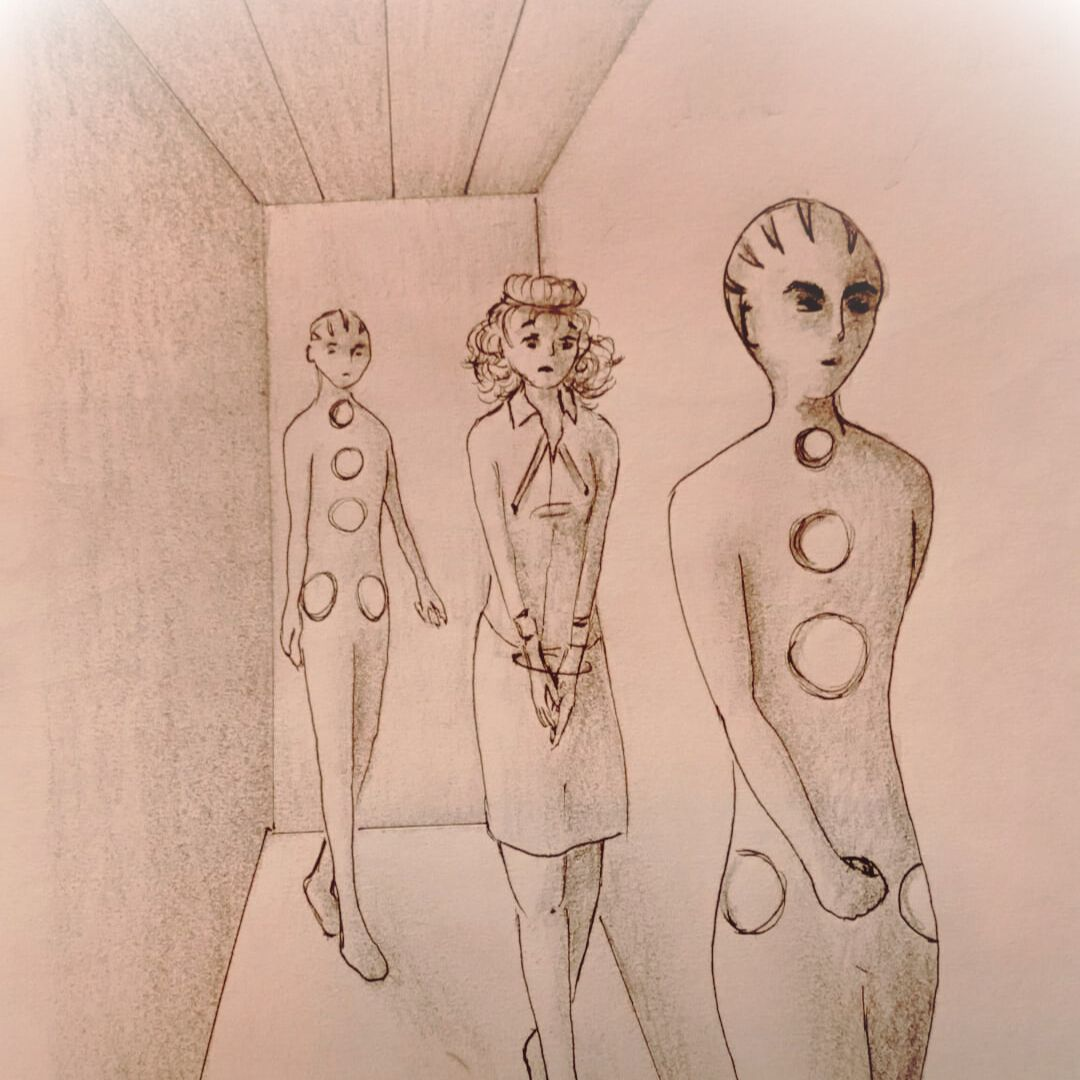
\includegraphics[width=\textwidth]{immagini/cnot_58.jpeg}} % Sostituisci con il nome del file immagine
\end{minipage}
\end{center}

\vspace{1em}
\begin{center}Caterina\end{center}
\hrule
\vspace{1em}

Queste strane guardie mi stavano scortando da questo Commissario. Prima il Supervisore, ora il Commissario. Volevo piangere. Passavamo per  corridoi freddi e squadrati, cunicoli improbabili, portali che non avevo mai neanche immaginato. Dove ero finita? Mi sentivo perduta. Il cuore mi batteva forte, non solo per la paura dell'ignoto, ma per qualcosa di più profondo che mi confondeva. Ripensai a come Mark si era alzato per difendermi, senza esitazione, e a come quella sicurezza e determinazione mi avessero dato una forza nuova, un senso di protezione che non avevo mai osato desiderare apertamente.

Mi resi conto, con una certa sorpresa, di quanto fosse importante per me sentirmi difesa, protetta da qualcuno capace di farsi avanti per me, di affrontare i pericoli con fermezza. Nella vita reale, non  mi ero mai permessa di esprimere questo bisogno; con il mio fidanzato, avevo sempre mostrato una facciata forte e indipendente, temendo di sembrare fragile o insicura. Quante volte aveva cercato di esserci per me, di offrirmi un sostegno che, ora lo capivo, avevo rifiutato senza rendermi conto del danno che arrecavo a entrambi?

Mi sentivo vulnerabile, ma per la prima volta accettavo quel sentimento come parte di me, come un segnale che non dovevo soffocare. Mentre avanzavo verso il Commissario, capii che forse, una volta fuori, avrei dovuto riconsiderare il mio rapporto con il mio fidanzato, permettendogli di prendersi cura di me, vivendola non come una debolezza, ma come una connessione più autentica e reciproca.


\chapter{Al cospetto del Commissario}

\begin{tcolorbox}[colback=gray!5,colframe=gray!80,title=\textbf{Scheda Informativa}]
\begin{itemize}
    \item \textbf{Luogo}: Sala centrale della \emph{Fault Tolerance Coding}
    \item \textbf{Giorno e ora}: Il tempo non è osservabile
    \item \textbf{Situazione}: Caterina viene condotta al cospetto del commissario per essere interrogata.
\end{itemize}
\end{tcolorbox}

\vspace{1em}
\begin{center}Caterina\end{center}
\hrule
\vspace{1em}


Fui condotta in una stanza ampia e riccamente arredata, un ambiente completamente diverso dall'austerità dei corridoi precedenti. La luce era calda e soffusa, e nell'aria c'era un profumo delicato, appena percepibile. Al centro della stanza, appoggiato con disinvoltura a una scrivania elegante e minimalista, mi aspettava il Commissario.

Quando lo vidi, rimasi per un istante sorpresa. Non aveva l'aspetto rigido e autoritario del Supervisore; al contrario, emanava un fascino naturale, quasi magnetico. Era giovane, elegante, e trasudava una sicurezza che sembrava più raffinata che arrogante. Quando mi avvicinai, lui mi salutò con un sorriso accennato e un cenno della mano.

\begin{dialogue}
\speak{Commissario} \enquote{Benvenuta.}
\end{dialogue}

Avvertii una strana sensazione di sollievo. Dopo le tensioni, la paura e l'interrogatorio con il Supervisore, la presenza del Commissario aveva qualcosa di rassicurante, quasi familiare. Non c'era traccia di minaccia nei suoi gesti o nel suo modo di parlare, e per la prima volta dall'inizio di questa strana avventura, mi sentii un po' più a mio agio.

\begin{dialogue}
\speak{Commissario} \enquote{Immagino che tu sia un po' spaesata.}
\end{dialogue}

Disse, sedendosi e indicando una sedia di fronte a lui, invitandomi a fare lo stesso.

\begin{dialogue}
\speak{Commissario} \enquote{Ti hanno trattata bene, spero?}
\end{dialogue}

Annuii, senza sapere bene cosa rispondere. Sembrava sinceramente interessato a me, e quando iniziò a parlare, il suo tono era calmo e coinvolgente.

\begin{dialogue}
\speak{Commissario} \enquote{Vedi, Caterina, posso comprendere quanto sia difficile trovarsi in un mondo così... diverso. Eppure, il fatto che tu sia riuscita ad arrivare qui, ad attraversare i limiti del nostro sistema, dimostra qualcosa di straordinario.}
\end{dialogue}

Si chinò leggermente in avanti, guardandomi dritto negli occhi.

\begin{dialogue}
\speak{Commissario} \enquote{Non capita a tutti di avere tale capacità.}
\end{dialogue}

Sentii il cuore battere più velocemente. Quelle parole sembravano colpirmi nel profondo. Come se potesse leggere i miei pensieri.

\begin{dialogue}
  \speak{Commissario} \enquote{So che hai delle qualità. La tua intelligenza si vede dai tuoi occhi.
  }
\end{dialogue}
\newpage
\section{L'interrogatorio}
\begin{center}
\begin{minipage}{0.7\textwidth}
    \centering
    \fbox{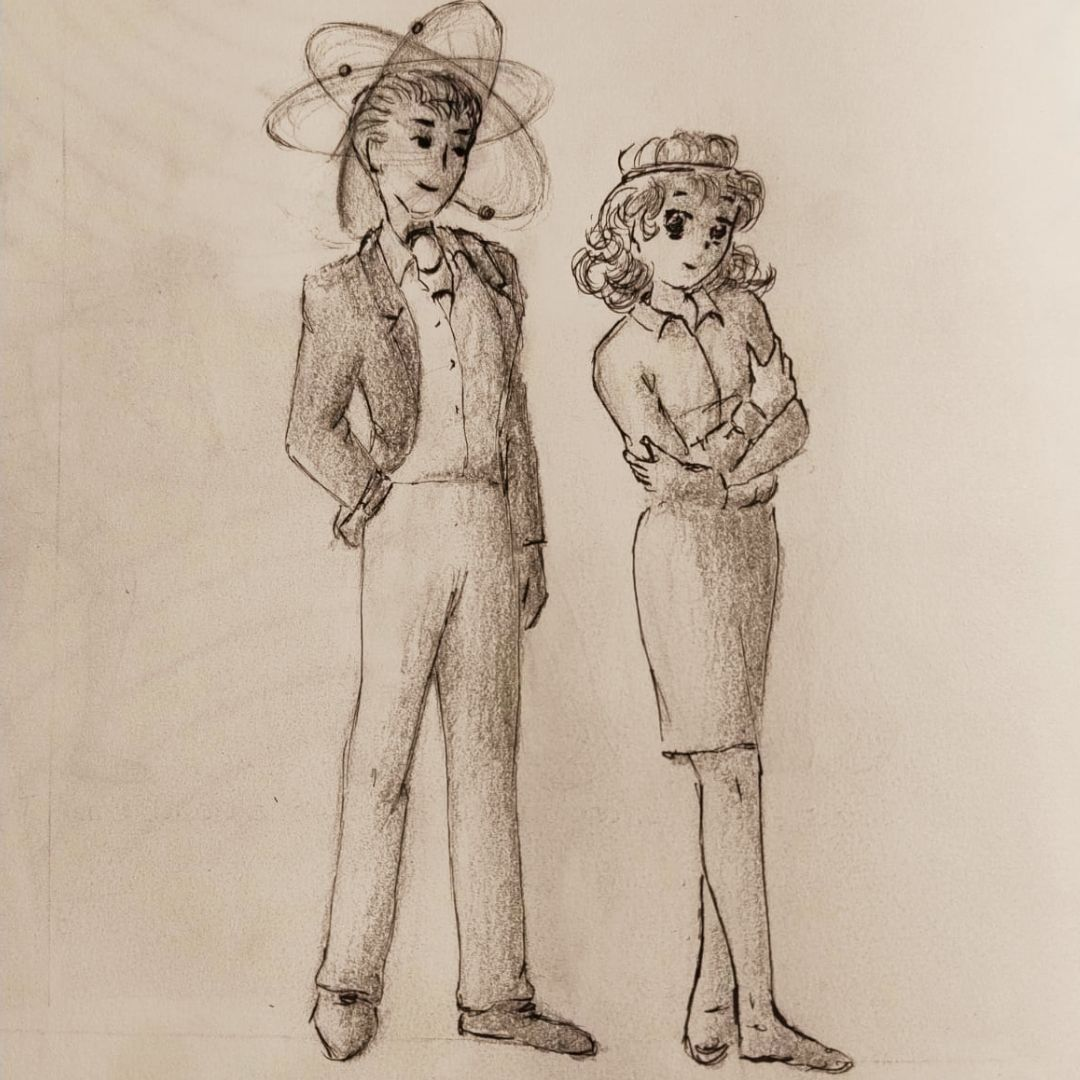
\includegraphics[width=\textwidth]{immagini/cnot_56.jpeg}} % Sostituisci con il nome del file immagine
\end{minipage}
\end{center}
Mi sentivo sempre più attratta dalle lusinghe del Commissario. La sua voce, calma e suadente, scorreva come un fiume tranquillo, facendo scivolare via le paure accumulate nel corso della giornata.

\begin{dialogue}
\speak{Commissario} \enquote{Sai, Caterina, il tuo arrivo qui è davvero straordinario. Persone come te, dotate di una mente brillante e di capacità eccezionali, sono esattamente ciò di cui abbiamo bisogno.}
\end{dialogue}

Le sue parole mi confondevano, e non potei fare a meno di sentirmi valorizzata. In un ambiente dove l'incertezza regnava sovrana e le mie fragilità erano amplificate, il Commissario sembrava rappresentare una boccata d'aria fresca. La sua presenza era rassicurante, e ogni parola pronunciata era un invito a credere che ci fosse un posto per me, un ruolo importante che potevo svolgere.

\begin{dialogue}
\speak{Commissario} \enquote{Non capita spesso di incontrare qualcuno con il tuo potenziale. Hai dimostrato di avere coraggio e determinazione, e non posso fare a meno di rispettare questo. È raro trovare individui che osano sfidare i confini del sistema. Il modo in cui ti sei esposta per proteggere un qubit sconosciuto mi ha colpito.}
\end{dialogue}

Sorpresa dalla sua considerazione, mi sentii quasi fluttuare. Era difficile resistere a un approccio così genuino, e la mia mente iniziò a fantasticare su ciò che avrei potuto realizzare in un mondo governato da una figura così carismatica. In quel momento, mi sentivo finalmente vista e compresa, come se ogni dubbio e ogni insicurezza stessero svanendo.

\begin{dialogue}
\speak{Commissario} \enquote{Immagina di lavorare insieme, di costruire qualcosa di grande. Non voglio solo il tuo aiuto, voglio che tu sia parte di un progetto straordinario. Un esercito di qubit non è solo un'idea; è un sogno che può diventare realtà, e tu potresti essere una delle colonne portanti di questo nuovo ordine.}
\end{dialogue}

Sentii il battito del cuore accelerare, mentre il mio pensiero tornava a quel mondo in cui i fallimenti del passato sembravano finalmente essere superati. Avevo sempre desiderato essere parte di qualcosa di più grande, ma non riuscivo a liberarmi dalla sensazione che ci fosse un costo nascosto in tutto ciò.

\begin{dialogue}
\speak{Caterina} \enquote{Ma come posso fidarmi di te?} domandai. \enquote{Cosa accadrebbe se ti rivelassi troppo? Se ti raccontassi tutto?}
\end{dialogue}

Il Commissario sorrise, un'espressione calda e sincera che sembrava promettere sicurezza.

\begin{dialogue}
\speak{Commissario} \enquote{Io non voglio manipolarti, Caterina. Voglio darti l'opportunità di mostrare al mondo ciò di cui sei capace. La fiducia è fondamentale, e ti assicuro che non ho intenzione di danneggiarti. Credimi, ho bisogno di te.}
\end{dialogue}

Sentivo la tensione svanire, mentre la mia mente veniva avvolta dalle sue parole affascinanti. Eppure, mentre mi lasciavo sedurre dal suo discorso, un ricordo tornò a galla. Le parole del mio fidanzato, che mi esortava a non aprirmi a chiunque, a mantenere le mie difese.

In quel momento, mi resi conto che stavo per rivelargli della presenza di Laura e del nostro legame dovuto forse al Noemografo. Decisi di fermarmi. L'idea di fidarmi completamente di un estraneo, per quanto affascinante, mi riempìva di incertezze.

Con un velo di determinazione, cercai di mantenere un po' di riserbo, ma lo feci con grazia.

\begin{dialogue}
\speak{Caterina} \enquote{Grazie per le tue parole, ma ho bisogno di tempo per riflettere,} dissi, cercando di mascherare il conflitto che mi stava formando nel cuore. Il commissario però continuava a pormi domande, prima semplici e dirette, ma poi più complesse ed incrociate, correvo il rischio di contraddirmi o di svelarmi.
\end{dialogue}

\section{La Fuga e la Trappola}

Decisi allora di cambiare approccio. Dovevo fingere di cedere, di lasciarmi sedurre dal Commissario. Iniziai a sorridergli, annuendo alle sue parole e lasciandomi trasportare dal suo discorso. Ogni tanto rispondevo con un cenno di assenso, un sussurro, facendogli credere di essere totalmente presa da lui. Sapevo che, se volevo avere una possibilità di fuga, dovevo essere convincente.

Il Commissario continuava a parlare, le sue parole erano suadenti, piene di fascino e di promesse.

\begin{dialogue}
\speak{Commissario} \enquote{Sai, Caterina, un giorno potresti avere un ruolo importante qui. Questo mondo ha bisogno di risorse come te, e con qualcuno come me al comando, potremmo realizzare grandi cose.}
\end{dialogue}

Il suo tono era quello di un leader, di un visionario che credeva in un futuro grandioso, e per un momento mi chiesi se non avesse davvero un piano così ambizioso.
Chiusi gli occhi e avvicinai le mie labbra socchiuse al suo volto sperando che facesse altrettanto. Ci baciammo delicatamente ma prima che i nostri corpi si scaldassero gli chiesi di lasciari il tempo per spogliarmi. Con galenteria il Commissario uscì dalla stanza lasciandomi sola. Ero riuscita nel mio intento, e questa era l'occasione che aspettavo per fuggire,  ma quando ci provai  mi ritrovai immobillizzata da una forza invisibile che mi tratteneva.

\begin{dialogue}
\speak{Commissario} \enquote{Mi avevi quasi convinto} disse, con un sorriso tranquillo.
\end{dialogue}

Prima che potessi reagire, fece un cenno e, quasi come per magia, una rete di particelle luminescenti cominciò a formarsi intorno a me. Cercai di muovermi, ma i miei polsi e caviglie furono bloccati in una morsa invisibile, un campo di energia mi stava immobilizzando.

\begin{dialogue}
\speak{Caterina} \enquote{Cosa stai facendo?} chiesi, cercando di mantenere la calma, ma la voce mi tremava leggermente.
\end{dialogue}

Il Commissario si avvicinò, e con un'espressione impassibile spiegò:

\begin{dialogue}
\speak{Commissario} \enquote{Non pensavi davvero di poter sfuggire, vero? Questa è la mia Ions trap, una trappola  che immobilizza ogni particella, anche le più ribelli,  all'interno del suo campo.}
\end{dialogue}

Sentivo la tensione elettrica scorrere lungo le braccia e le gambe, un formicolio che sembrava trattenere ogni mio movimento. Mi sentivo impotente, e il cuore iniziò a battere forte, mentre la consapevolezza della mia cattività mi calava addosso. Il Commissario mi fissava senza pietà, e per la prima volta percepii in lui una crudeltà che era stata nascosta dietro le sue lusinghe.

\begin{dialogue}
\speak{Commissario} \enquote{Non sei altro che una pedina in questo gioco. Pensavi di poter giocare con me?  Ora vedremo chi di noi ha il vero potere.}
\end{dialogue}

Abbassai lo sguardo, cercando di non mostrare il mio terrore. Sapevo che ora sarei stata completamente in balia del Commissario, e ogni speranza di fuga sembrava svanita in quel campo di ioni che mi imprigionava.


\chapter{Le urla del collasso}
\begin{tcolorbox}[colback=gray!5,colframe=gray!80,title=\textbf{Scheda Informativa}]
\begin{itemize}
    \item \textbf{Luogo}:  \emph{Quantum Measurement}
    \item \textbf{Giorno e ora}: Il tempo non è osservabile
    \item \textbf{Situazione}: Laura e Marley stanno fuggendo.
\end{itemize}
\end{tcolorbox}

\vspace{1em}
\begin{center}Laura\end{center}
\hrule
\vspace{1em}

 Marley e io fuggivamo attraverso gli stretti corridoi. L'eco metallico dei nostri passi si avvicinava alla frequenza del mio cuore. Improvvisamente, una serie di urla strazianti squarciò il silenzio. Era un suono agghiacciante, simile a un coro di disperazione proveniente da un'altra dimensione. Mi fermai di colpo, il cuore mi martellava nel petto.

\begin{dialogue}
\speak{Laura} \enquote{Cosa sta succedendo?} chiesi, cercando di mantenere la calma nonostante il terrore che mi pervadeva.

\speak{Marley} \enquote{È il suono dei qubit che collassano} rispose Marley, il volto pallido e teso. \enquote{Stanno subendo le conseguenze del processo di misura. Non riescono a mantenere il loro stato, e quando questo accade... l'effetto è devastante.}
\end{dialogue}

Una stretta gelida mi avvolse lo stomaco. Quelle urla sembravano avere il potere di destabilizzare anche i qubit più stabili.

\begin{dialogue}
\speak{Laura} \enquote{E Caterina?} domandai, la voce incrinata dall'angoscia. \enquote{Dove si trova adesso?}

\speak{Marley}  \enquote{Se non è già stata portata nel \textit{Faulty Qubit Space}, è probabile che sia ancora nel \textit{Fault Tolerance Coding}. Ma dobbiamo muoverci in fretta, dal FQS non potremo più salvarla.}

\speak{Laura} \enquote{Agiamo subito!} esclamai, sentendo l'urgenza crescere dentro di me.

\speak{Marley} Prese un respiro profondo. \enquote{La verità è che, per trovare Caterina, dovremmo prima sconfiggere il Commissario. È sicuramente sua prigioniera.}

\speak{Laura} Feci un passo indietro, incredula. \enquote{Sconfiggere il Commissario? Ma chi è il Commissario?}

\speak{Marley} \enquote{Un traditore. Vuole costruire un sistema parallelo per spodestare il \textit{Quantum Master Program}} rispose. \enquote{\'E l'unico modo. Se vogliamo salvare Caterina e gli altri, dobbiamo agire.}
\end{dialogue}

Mentre cercavamo un nascondiglio tra le ombre del \textit{Quantum Measurement}, un suono metallico e ronzante ci fece sobbalzare. Dai corridoi oscuri alle nostre spalle, due droni \textit{CH4} comparvero, fluttuando come presenze spettrali. Ciascun drone, con i suoi quattro rotori disposti a tetraedro, emetteva una luce soffusa che si rifletteva sulle pareti, mentre due figure scure erano in sella: gli agenti della \textit{Quantum Control Electronics}, inviati per trovarci.

Ci accovacciammo dietro una serie di circuiti e componenti, trattenendo il fiato. I due agenti atterrarono con precisione e, scendendo dai droni, iniziarono a perlustrare l'area. I loro volti erano inespressivi, ma gli occhi scrutavano attentamente ogni dettaglio,  non andavano a caso e ci avrebbero scoperto.  Non avevamo molto tempo. Dovevamo agire in fretta, o saremmo state scoperte.

Marley mi lanciò uno sguardo, cercando una direzione sicura, ma l'intero spazio sembrava chiuso, senza vie di fuga evidenti. Restammo in attesa, pronte a muoverci al primo segnale, sperando di riuscire a eludere gli agenti e sfuggire alla sorveglianza della \textit{Quantum Control Electronics}.

\section{I due agenti}
\vspace{1em}
\begin{center}PzIA\end{center}
\hrule
\vspace{1em}
Gli agenti si muovono con movimenti misurati, esaminando l'area circostante. Uno dei due abbassa la voce e si rivolge al compagno.

\begin{quote}
\enquote{Pensi che possano essersi nascoste nel settore di stabilizzazione dei qubit? Quel posto è praticamente un labirinto,} sussurra, lanciando uno sguardo preoccupato ai droni in standby accanto a loro.
\end{quote}

Il secondo agente mantiene lo sguardo fisso su ogni angolo e su ogni ombra.

\begin{quote}
\enquote{Possibile. Ma se sono abbastanza furbe, potrebbero aver scelto un luogo meno ovvio} risponde.
\end{quote}

Il primo agente annuisce, mostrando segni di tensione.

\begin{quote}
\enquote{Meglio non fare errori. Sai cosa è successo all'ultima squadra che ha fallito una missione sotto gli occhi del Supervisore...}
\end{quote}

Il secondo agente interrompe, con un leggero brivido.

\begin{quote}
\enquote{Non ricordarmelo. Il Supervisore non perdona. E peggio ancora, c'è il \textit{Quantum Master Program} che supervisiona tutto. Nessuna deroga alla coerenza, nessuna possibilità di sfuggire alle direttive.}
\end{quote}

Entrambi gli agenti rivolgono uno sguardo ai droni, gioelli della nanotecnologia sotto la loro diretta responsabilità. Abbandonarli era sempre un rischio. Dopo un momento di silenzio, il secondo agente riprende con voce più ferma.

\begin{quote}
\enquote{Concentriamoci. Dobbiamo trovarle prima che la situazione sfugga di mano. Altrimenti saremo noi a pagarne le conseguenze.}
\end{quote}

Il primo agente annuisce nuovamente, prendendo un respiro profondo.

\begin{quote}
\enquote{Sì, hai ragione. Controlliamo quest'area con attenzione. E speriamo che siano più vulnerabili di quanto ci aspettiamo.}
\end{quote}

\section{La Fuga sul Drone CH4}
\vspace{1em}
\begin{center}Laura\end{center}
\hrule
\vspace{1em}

 Il cuore mi si appesantiva al pensiero del rischio imminente. Eppure, dentro di me, qualcosa si stava risvegliando.

\begin{dialogue}
\speak{Laura} \enquote{Potremmo fuggire con uno di quei droni \textit{CH4}. Potremmo saltarci sopra e raggiungere il \textit{Fault Tolerance Coding} prima che sia troppo tardi!}
\end{dialogue}

Marley scosse la testa, il viso cupo.

\begin{dialogue}
\speak{Marley} \enquote{Non è così semplice. Abbiamo provato a usarli, ma non ci siamo mai riusciti. I droni sono dotati di sistemi di sicurezza e le probabilità di farci scoprire sono alte. Inoltre il passaggio da qui verso il \textit{Fault Tolerance Coding} è sorvegliato da un filtro molecolare, non potremmo mai superarlo a bordo di un $CH_4$.}
\speak{Laura} \enquote{Possiamo andare a piedi?}
\speak{Marley} \enquote{Fuori discussione....}
\speak{Laura} \enquote{Esiste un'alternativa?}
\speak{Marley} \enquote{Possiamo passare per la CCU, se riusciamo a superarla proseguire verso la \textit{Quantum Control Electronics}  e quindi rientrare nel QA. Da li esiste un accesso non controllato verso il \textit{Fault Tolerance Coding}, ma...}
\speak{Laura} \enquote{Ma cosa? C'è qualche problema?}
\speak{Laura} \enquote{Niente. Meglio affrontare i problemi quando si pongono di fronte} concluse. Non aggiunsi altro. 
\end{dialogue}

Guardai il drone \textit{CH4}, un oggetto affascinante e al contempo intimidatorio.

\begin{dialogue}
\speak{Laura} \enquote{Dobbiamo provare, non vedo alternative} dissi indicando il drone.
\end{dialogue}

\begin{dialogue}
\speak{Marley} Marley cercò di mantenere il tono calmo, ma parlò senza mai prendere fiato: \enquote{Laura, ascolta. Non è solo questione di scappare. Dobbiamo avere un piano. Quel drone non ci porterà lontano se non abbiamo il controllo. Non possiamo permettere che i nostri sforzi siano vani.}
\end{dialogue}



%---from here

%--- to here

Strinsi i denti e scrutai il drone: qualcosa doveva pur esserci. Un'idea si faceva largo tra il caos.

\begin{dialogue}
\speak{Laura} \enquote{Aspetta... quel drone, ha la geometria di una molecola di metano. Se è davvero così, allora ha spin totale 1. Forse possiamo controllarlo modificando la proiezione dello spin lungo l'asse Z.}
\end{dialogue}

Marley mi guardò, gli occhi spalancati.

Forse arrossii.

\begin{dialogue}
\speak{Laura} \enquote{Ho solo... ho studiato queste cose. Ho messo insieme qualche indizio. Forse mi sbaglio...}
\end{dialogue}

Marley iniziò a sospettare che non fossi del tutto come lei. E io? Io cominciavo a sospettare che forse... non fossi nemmeno più del tutto nel mio mondo.


\begin{dialogue}
\speak{Marley} \enquote{Sei una \textit{Quantum Crafter}, vero?}
\end{dialogue}

Arrossii leggermente.

\begin{dialogue}
\speak{Laura} \enquote{Non è il momento di parlarne. Dobbiamo agire ora!}
\end{dialogue}

\begin{center}
\begin{minipage}{0.7\textwidth}
    \centering
    \fbox{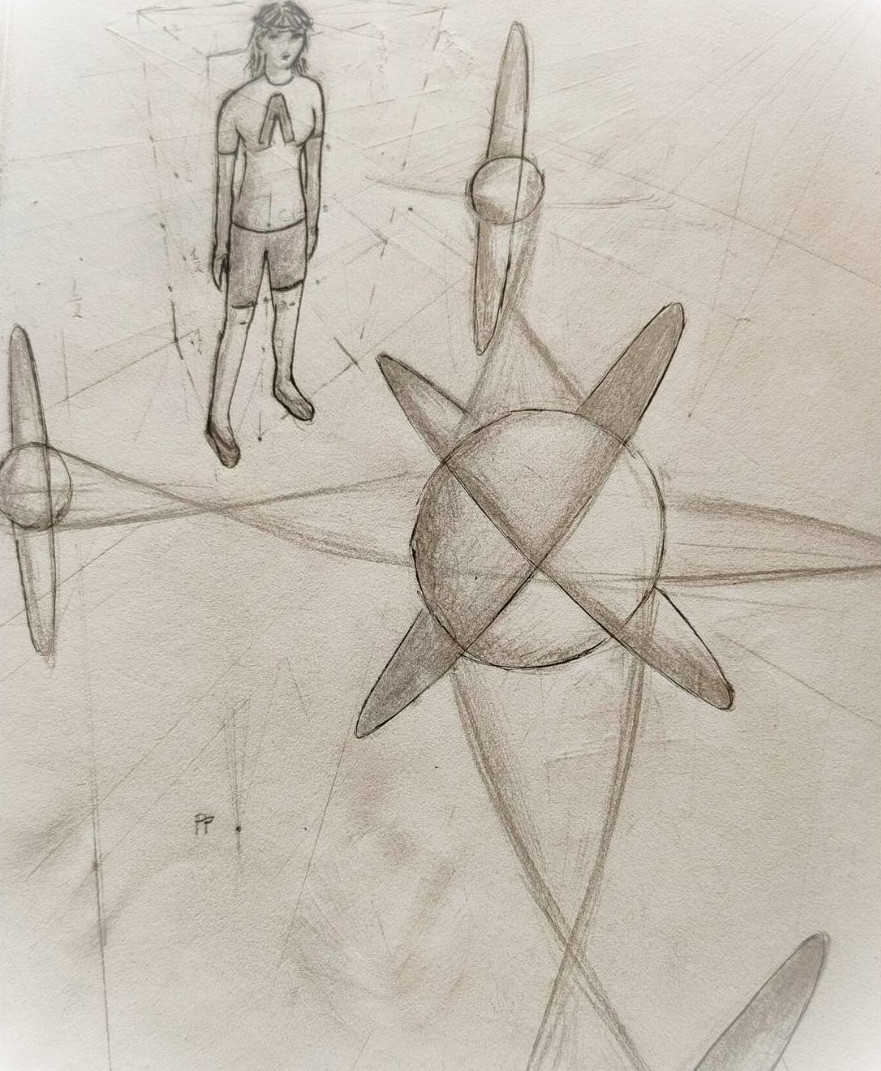
\includegraphics[width=\textwidth]{immagini/cnot_50.jpeg}} % Sostituisci con il nome del file immagine
\end{minipage}
\end{center}

\section{Il Piano di Fuga}

\begin{dialogue}
\speak{Laura} \enquote{Quello sembra un sistema a spin totale 1. Probabilmente si manovra modificando la proiezione dello spin lungo l’asse Z. Dobbiamo provarci!}
\end{dialogue}

Per un attimo mi vidi dall'esterno, sospesa tra paura e coraggio. Mi osservavo da fuori di me. Negli occhi brillava la determinazione. Volevo affrontare il mio destino.


Marley, pur impressionata dalla mia sicurezza, sembrava esitante.

\begin{dialogue}
\speak{Marley} \enquote{Laura, aspetta! Non abbiamo idea di come farlo funzionare. Potrebbe essere troppo pericoloso!}
\end{dialogue}

Ma non potevo permettermi di esitare. Ogni istante di inattività poteva significare la perdita definitiva di Caterina. Mi avvicinai al drone con il cuore che batteva forte per la paura, ma anche per il richiamo dell'azione.

Mi lanciai sull'agente più vicino, che cadde a terra, colto di sorpresa. Senza esitazione, saltai verso il drone, ma ovviamente non me l'avrebbe regalata così facilmente. Mi afferrò per una caviglia facendomi rovinare a terra spinta dal mio stesso impulso. Il drone era ad un soffio dovevo solo liberarmi da quella stretta prima che arrivasse anche l'altro. Sentii un urlo alle mie spalle, qualcosa o qualcuno lo aveva colpito. Ma certo, Marley! Aveva trovato la forza e mi aveva siutata. Saltammo  sul drone.  Afferrai i comandi orbitali. Il carbonio era freddo, gli atomi di idrogeno tesi al limite: non era il massimo, ma poteva andare. Non era il mio scooter, ma potevamo farcela!




\begin{center}
\begin{minipage}{0.7\textwidth}
    \centering
    \fbox{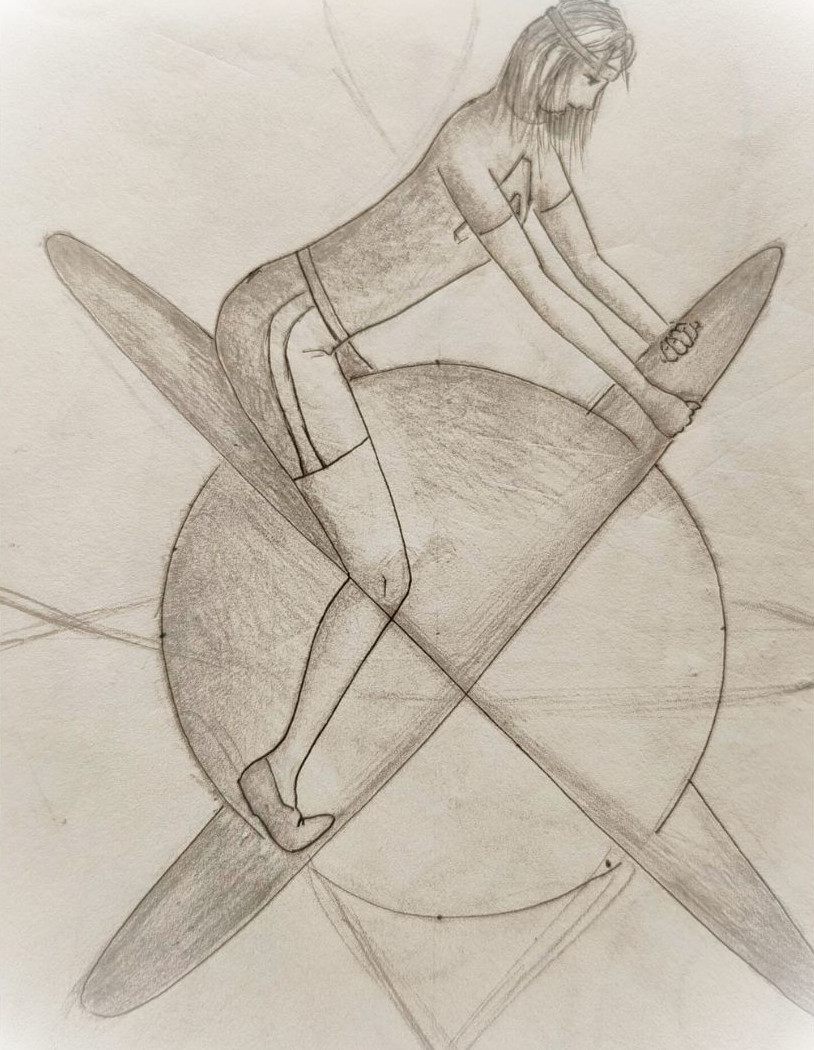
\includegraphics[width=\textwidth]{immagini/cnot_51.jpeg}} % Sostituisci con il nome del file immagine
\end{minipage}
\end{center}


\begin{dialogue}
\speak{Laura} \enquote{Non possiamo fallire. Insieme, possiamo farcela!}
\end{dialogue}

Marley annuì, e le paure che l'avevano trattenuta iniziarono a svanire.

\begin{dialogue}
\speak{Marley} \enquote{D'accordo, Laura. Facciamo in modo che funzioni. Se siamo rapide, possiamo arrivare al \textit{Fault Tolerance Coding} prima che trasferiscano Caterina!}
\end{dialogue}

Con il cuore in gola e la determinazione che pulsava come un'onda di energia, attivai il drone. La superficie  brillava mentre gli oribitali iniziavano a girare, emettendo un sibilo potente che vibrava nell'aria circostante. L'adrenalina scorreva potente, e mentre il drone si sollevava da terra, una nuova speranza si accese dentro di me. Eravamo pronte a lanciarci verso l'ignoto, verso il salvataggio della nostra amica.

\begin{dialogue}
\speak{Marley} \enquote{Vai ora, dirigiti verso quel condensatore, lì c'è il passaggio per la CCU.} In quel momento sentii l'energia che provavo quando da bambina mio padre mi leggeva Salgari. ``Andiamo, papà'' pensai, mentre il suo ricordo mi sfiorò per un istante.
\end{dialogue}


\chapter{La fuga di Laura}
\vspace{1em}
\begin{center}PzIA\end{center}
\hrule
\vspace{1em}

%---cronaca inizio
\textbf{Signore e signori, l'azione si infiamma!} L'agente colpito da Laura è a terra, mentre l'altro scatta all'inseguimento!
I droni sfrecciano nei corridoi del QM, come in una finale mozzafiato di coppa quantistica!

\emph{Attenzione!} Dal centro di controllo arriva una comunicazione gelida che blocca il fiato ai nostri concorrenti.
\begin{dialogue}
\speak{Supervisore} ``Non tollero fallimenti'' annuncia, implacabile come sempre.
\end{dialogue}
\textbf{Colpo di scena!} L'agente a terra viene disattivato all'istante. Fuori gara! Il sistema non ammette errori e il Supervisore non conosce pietà.

L'agente superstite, terrorizzato, stringe i comandi del suo drone. Non può permettersi di perdere, non oggi!

%---cronaca fine


\section{Il Drone \textit{CH4}}

Laura guida il drone \textit{CH4} con una destrezza sorprendente!
Sta per lasciare il QM per dirigersi verso la CCU ma deve attraversare il dielettrico del condensatore.

Il suo sguardo è determinato. Non c'è incertezza. Deve attraversare il dielettrico. Ecco che Laura prepara il suo drone per evitare che interagisca con il campo elettrico accumulato. Attenzione, è un momento cruciale: il condensatore è carico, come una molla pronta a scattare. Ogni movimento sbagliato potrebbe provocare un arco elettrico devastante!

Laura regola la velocità del drone, impostando con precisione il livello di isolamento dei rotori. \textit{Perfetto, sta calcolando il punto d'ingresso.} Ecco che il drone si avvicina al confine del dielettrico. Gli strumenti a bordo stanno analizzando le proprietà del campo elettrico—un lavoro di millisecondi, ma ogni dato conta.

E ora… ora accelera! Il drone CH4 si lancia nel dielettrico. L’aria sembra vibrare attorno al campo elettrico; una leggera scarica illumina il percorso del drone. Tutto si svolge in una frazione di secondo: Laura tiene saldamente i comandi, corregge la traiettoria al volo. Sta dosando con precisione chirurgica il flusso di energia attraverso i circuiti del drone per evitare sovraccarichi.

Ma attenzione! Un lieve squilibrio nel campo! Il drone trema, i sensori segnalano un picco di tensione! Laura risponde prontamente, modificando l’angolo di rotazione dei rotori. Una mossa audace, perfettamente sincronizzata. Il drone attraversa il dielettrico in un lampo di luce.


\begin{tcolorbox}[colback=gray!5,colframe=gray!80,title=\textbf{Scheda Informativa}]
\begin{itemize}
    \item \textbf{Luogo}: \emph{Classical Control Unit}
    \item \textbf{Giorno e ora}: Il tempo non è osservabile
    \item \textbf{Situazione}: Laura e Marley puntano verso la QCE.
\end{itemize}
\end{tcolorbox}


\textit{È incredibile! Ce l'ha fatta!} Laura emerge dall’altra parte del condensatore con una traiettoria impeccabile. Il drone è intatto, i sensori segnalano la stabilità ripristinata. Gli osservatori non osservano per non influenzare le traiettorie e Laura non si concede il lusso di rilassarsi.

Sta già pianificando il prossimo passo, un altro ostacolo da superare nel labirinto della Classical Control Unit. Un’impresa straordinaria, un controllo assoluto: Laura dimostra ancora una volta che nulla può fermarla.

Che momento epico!


Ogni componente rappresenta un ostacolo: chip integrati, condensatori, minuscole resistenze che formano una vera e propria giungla elettronica. Ma Laura li evita con precisione millimetrica, sfruttando la sua conoscenza approfondita dei circuiti. \textbf{È una vera maestra del volo!}

Con il cuore in gola, sterza il drone con movimenti rapidi e sicuri. Alle sue spalle, il rombo minaccioso del drone dell'agente si avvicina. \emph{L'inseguimento è serrato!} La sua familiarità con i percorsi elettronici le permette di anticipare ogni manovra, sfuggendo abilmente ai tentativi dell'agente di raggiungerla.

\textbf{Ed ecco un colpo di scena!} Laura incalzata dal drone dell'agente deve trovare l'ingresso principale per la QCE. Mentre vola radente al rame dei PCB nota un ingresso segnato con una grande \textbf{H} incisa sopra. Qualcosa in quella lettera emana un'energia misteriosa, come se racchiudesse un segreto.

\begin{quote}
\enquote{Marley, guarda!} esclama, \enquote{Qualcosa mi dice che potrebbe essere un'entrata.}
\end{quote}

Marley segue lo sguardo di Laura e sussurra con terrore:

\begin{quote}
\enquote{Aspetta, quello è un portale quantistico, non è un accesso elettronico...}
\end{quote}

Ma Laura indirizza il drone verso l'ingresso segnato dalla lettera \textbf{H}. \emph{Non c'è tempo da perdere!} Le pareti del portale sono lisce e scintillanti, emettono una luce tenue che vibra al ritmo del loro avvicinarsi.

\textbf{Siamo al momento decisivo!} Riusciranno Laura e Marley a sfuggire all'inseguimento e a scoprire cosa si cela oltre il portale? \emph{Restate sintonizzati per l'esito di questa emozionante corsa verso l'ignoto!}

\begin{tcolorbox}[colback=gray!5,colframe=gray!80,title=\textbf{Scheda Informativa}]
\begin{itemize}
    \item \textbf{Luogo}: Sala centrale della \emph{Fault Tolerance Coding}
    \item \textbf{Giorno e ora}: Il tempo non è osservabile
    \item \textbf{Situazione}: Caterina è imprigionata nella Paul Trap.
\end{itemize}
\end{tcolorbox}

\vspace{1em}
\begin{center}Caterina\end{center}
\hrule
\vspace{1em}

Mi ritrovo intrappolata qui, in questa realtà che non riesco a decifrare. Ogni passo che ho fatto per arrivare a questo punto mi sembra adesso carico di una testardaggine cieca. Perché dovevo insistere così tanto? Perché non potevo semplicemente accettare la spiegazione di Eva e andare avanti? Mi chiedo continuamente se avrei potuto lasciar perdere, se avrei potuto evitare di spingermi così oltre per capire cosa fosse successo a quel maledetto colloquio di lavoro.

Ma no, Caterina non può lasciar perdere. Devo sapere tutto, devo avere le risposte, devo controllare. E ora guarda dove mi ha portato tutto questo. Un guaio più grande di me, più grande di quanto avrei mai potuto immaginare. Non solo sono intrappolata in questo sistema, ma la mia ostinazione mi ha separata da Laura, l’unica persona che avrebbe potuto aiutarmi a trovare una via d’uscita.

E tutto per seguire Mark. Perché? Perché ho pensato che fosse la scelta giusta, che fosse lui a darmi quelle risposte che cercavo disperatamente. Ma in realtà, Mark mi ha solo allontanata da Laura. Laura, che era la mia ancora, la mia speranza, la mia connessione con il mondo reale. Ora sono sola, in questo labirinto quantistico, e ogni passo mi sembra un peso, ogni decisione un errore che non posso correggere.

Mi sento come se avessi tradito non solo Laura, ma anche me stessa. Non ho saputo ascoltare chi cercava di aiutarmi, chi era davvero dalla mia parte. E ora la mia testardaggine, la mia ossessione per il controllo, mi ha lasciata qui, con nulla di certo e nessuna via d'uscita.

Eppure, una parte di me si rifiuta di arrendersi. Se Laura mi ha insegnato qualcosa, è che la volontà può aprire porte che sembrano sigillate. Ma per ora, mi sento persa. Persa nel mio stesso labirinto di decisioni sbagliate.

\begin{dialogue}
\speak{Caterina} \enquote{Ma come ho fatto a finire così? Tutto per colpa della mia stupida testardaggine. Se solo avessi lasciato perdere quel colloquio, non sarei qui!} Continuavo a lamentarmi sperando che arrivasse Laura a salvarmi. \enquote{E ora Laura è lontana, chissà dove. L'unica persona che avrebbe potuto aiutarmi, e io l'ho persa.}

\speak{Shor} \enquote{Ehi, ragazza... sei umana?} Una voce sommessa e calma si fece strada tra il silenzio, facendomi sobbalzare.

\speak{Caterina} \enquote{Chi parla? Chi sei?}

\speak{Shor} \enquote{Sono il professor Shor.} La sua voce sembrava avvolta da una calma strana, quasi irreale. \enquote{Non volevo spaventarti, ma devo sapere... sei davvero umana?} mi chiese. Ma che senso aveva questa domanda, cosa dovrei essere se non umana?

\speak{Caterina} \enquote{Sì, lo sono. Ma...} 

\speak{Shor} \enquote{Sei in un computer. Sei intrappolata come me, immagino. Ora dimmi: chi sei, e perché sei qui?}

\speak{Caterina} Esitai per un momento. \enquote{Mi chiamo Caterina. Ero a un colloquio di lavoro. Qualcosa non quadrava, così ho insistito per avere risposte. Mi hanno trascinata in questo... computer? E ora sono intrappolata. Non so come tornare indietro.}

\speak{Shor} \enquote{Capisco. Questo sistema non perdona la curiosità, ma la tua presenza qui è un'anomalia interessante. E Laura, questa Laura che hai menzionato? Anche lei è qui?}

\speak{Caterina} \enquote{Sì, o almeno lo era. Ma l'ho persa e sono rimasta sola.}

\speak{Shor} \enquote{Ascoltami bene, Caterina. Non sei sola, e non è tutto perduto. Se Laura è qui, troverò un modo per contattarla. La connessione tra due umani è una forza potente, anche in un sistema come questo. L'amore e l'amicizia sono più forti dell'entanglement. Raccontami tutto quello che sai. Potrebbe esserci un dettaglio che possiamo sfruttare.}

\speak{Caterina} \enquote{Davvero puoi trovarla?}

\speak{Shor} \enquote{Nulla è certo in questo mondo... certo tranne le misure di sistemi puri in un autostato... Ma questo non c'entra nulla, o meglio forse vuoi che ti parli dell'entropia quantistica?}
\speak{Caterina} \enquote{Professore, può aiutarmi?}
\speak{Shor} \enquote{Certo scusami, stavo prendendo la tangente... Senti prova a pensare intensamente a Laura. Le connessioni affettive si trasformano in canali di comunicazione quantistici. Se siete amiche come mi hai detto riusciremo a creare una connessione.}
\end{dialogue}

Mi sforzai di concentrarmi su Laura, come mi aveva chiesto Shor. Era un compito strano, pensare così intensamente a qualcuno, quasi come se dovessi richiamarla da un luogo lontano. Mi impegnai a visualizzarla: il suo viso deciso, i lineamenti che ispiravano sicurezza, quel modo di guardare le cose come se niente potesse davvero spaventarla.

Mentre lo facevo, un pensiero mi attraversò la mente. Il noemografo. Quel dispositivo che avevamo provato insieme, quasi per gioco. Quando lo avevamo usato, c'era stato un momento in cui avevo avuto l’impressione di sentire i suoi pensieri, o forse era lei che sentiva i miei. E se fosse quello? Se fosse stato il noemografo a creare questa connessione, qualcosa che ci legava anche qui, in questo mondo assurdo?

L’idea mi diede un brivido, ma anche una nuova speranza. Forse non era tutto perduto. Forse c'era un modo per raggiungerla, per fare arrivare il mio pensiero fino a lei. "Ci sto provando, Shor," mormorai, cercando di rendere Laura sempre più presente nella mia mente. "Spero davvero che basti."

\section{Attraversamento del Gate di Hadamard}


\vspace{1em}
\begin{center}Laura\end{center}
\hrule
\vspace{1em}

\enquote{Il portale H è di fronte a noi. Ora devo centrare l'apertura senza che uno degli atomi di idrogeno vada a cozzare} pensai.
Trassi un respiro profondo e senza chiudere gli occhi diressi il drone verso l'apertura superiore tra il soffitto e la gambina della H.



\begin{dialogue}
\speak{Marley} \enquote{Wow! Laura! \'E bellissimo} disse mentre superavamo il portale {è come se mi risvegliassi da un torpore!}
\end{dialogue}


\begin{tcolorbox}[colback=gray!5,colframe=gray!80,title=\textbf{Scheda Informativa}]
\begin{itemize}
    \item \textbf{Luogo}: \emph{Quantum Control Electronics}
    \item \textbf{Giorno e ora}: Il tempo non è osservabile
    \item \textbf{Situazione}: Laura e Marley puntano al QA.
\end{itemize}
\end{tcolorbox}


Ma per me, l'esperienza era completamente diversa. Avevo la sensazione che il mio essere fosse diviso in infiniti stati, come se la mia mente stesse tentando di occupare più spazi contemporaneamente. Era come se il portale mi avesse trasformata in una miriade di diverse me stessa, un'esperienza che mi destabilizzava. La percezione di ogni pensiero, di ogni intenzione, si spezzava in un caleidoscopio di alternative.

Mi resi conto di cosa rappresentava quella H. Il portale era un \textit{gate} di Hadamard, un passaggio che mi aveva gettata in uno stato di sovrapposizione, dove ogni cosa era simultaneamente possibile e impossibile. Lottavo per mantenere il controllo della mia coscienza, ma il peso di pensieri contrastanti mi oscurava la mente.
Persi il controllo del $CH_4$ e per un attimo piombammo verso un transistor interrato. Durò poco. La voce di Caterina mi suonò nel cervello: ``Laura, aiutami!'' Era come se lei fosse proprio lì, a pochi passi da me.
Ripresi il controllo del drone, continuai a guidare, ma mi sentivo confusa, come se stessi pensando a una cosa e al suo opposto nello stesso momento. Ogni decisione sembrava incerta,  ogni scelta aveva infinite ramificazioni e ogni rotta una probabilità diversa.

\begin{dialogue}
\speak{Laura} \enquote{Mi sento intrappolata tra due pensieri} mormorai, il volto teso e i movimenti meno sicuri.
\end{dialogue}

Marley mi guardava preoccupata, notando il cambiamento nel mio sguardo.

\begin{dialogue}
\speak{Marley} \enquote{Laura, stai bene?} chiese.
\end{dialogue}

\begin{dialogue}
\speak{Laura} \enquote{Non so... è come se stessi vedendo tutto da due prospettive opposte. Non so più cosa sia reale e cosa non lo sia} risposi cercando di mantenere la concentrazione.
\end{dialogue}

Nonostante il disorientamento, cercavo di rimanere concentrata, sapendo che il pericolo era ancora alle nostre spalle.
\newpage
\section{Concentrarsi sulla fuga}
\vspace{1em}
\begin{center}PzIA\end{center}
\hrule
\vspace{1em}

\begin{center}
\begin{minipage}{0.7\textwidth}
    \centering
    \fbox{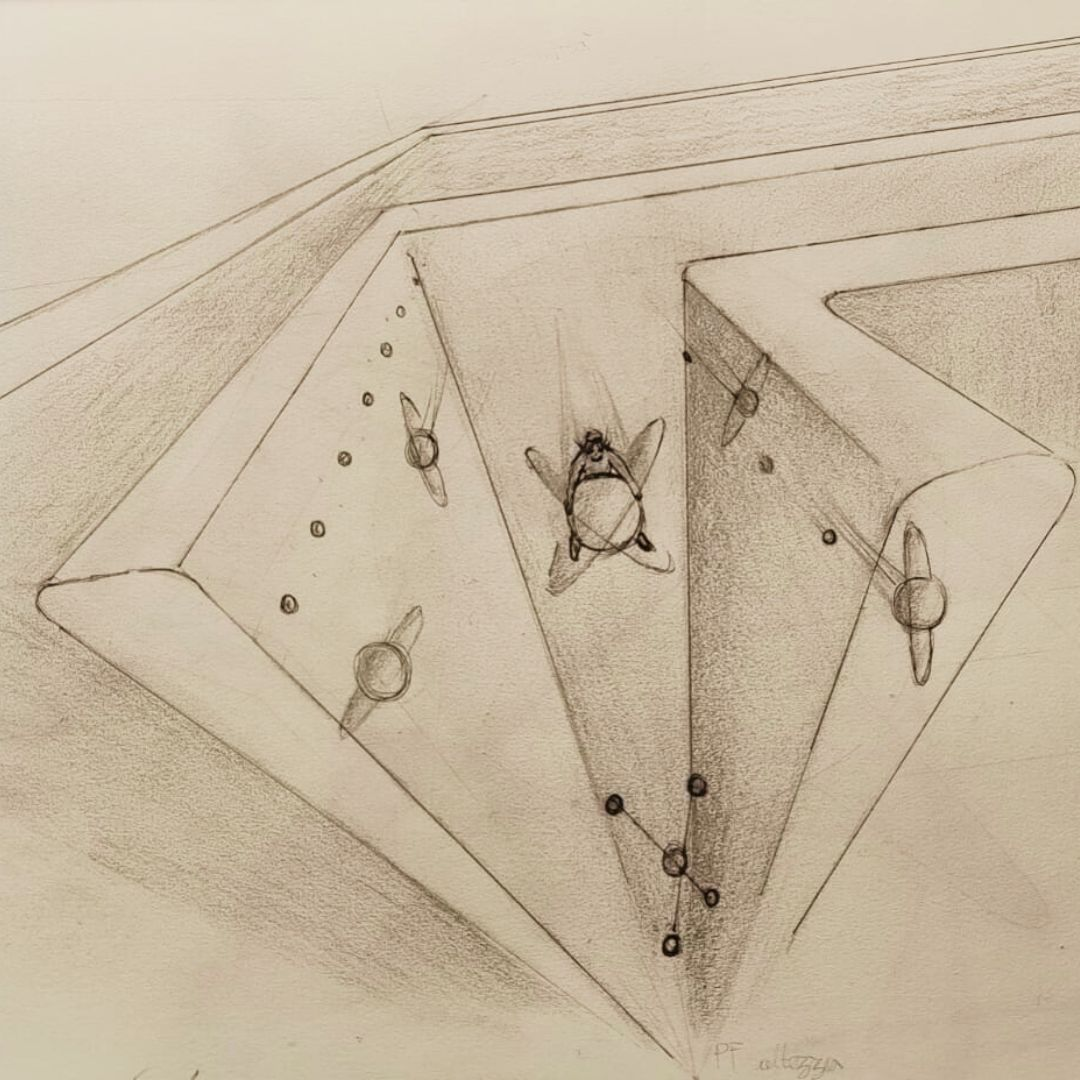
\includegraphics[width=\textwidth]{immagini/cnot_59.jpeg}} % Sostituisci con il nome del file immagine
\end{minipage}
\end{center}

Dietro di loro, l'agente in inseguimento rileva la posizione di Laura e Marley. In un ultimo tentativo di catturarle, modifica la configurazione del suo drone \textit{CH4}. I quattro rotori, precedentemente disposti in formazione tetraedrica, iniziano a ruotare, allineandosi su un unico piano.

\textbf{Allerta:} la nuova configurazione aumenta significativamente la manovrabilità e la stabilità del drone, migliorando la capacità di inseguimento dell'agente. La formazione tetraedrica, che offriva potenza e controllo verticale, è ora sostituita da una disposizione che consente maggiore agilità e velocità orizzontale.

Marley mostra segni di ansia crescente.

\begin{dialogue}
\speak{Marley} \enquote{Laura, sta guadagnando terreno!} esclama.
\end{dialogue}

Laura registra la situazione critica.

\begin{dialogue}
\speak{Laura} ``Credo di avere un asso nella manica,'' disse con un sorriso determinato. ``vedi quel diodo...  noi passiamo nel verso giusto, e l'agente ci sbatterà contro!''

\end{dialogue}

Il suo battito cardiaco accelera, ma mantiene la concentrazione. Nonostante la confusione causata dal \textit{gate} di Hadamard, cerca di superare l'instabilità mentale per focalizzarsi sulla fuga e sul salvataggio di Caterina.

La distanza tra i due droni si riduce rapidamente. L'agente ottimizza le traiettorie, anticipando le mosse di Laura.

\textbf{Situazione critica:} se l'agente le raggiunge, la missione di Laura e Marley potrebbe fallire.

Le probabilità di successo diminuiscono. Tuttavia, Laura sfrutta la sua conoscenza dei percorsi interni entrando nel diodo come progettato. L'agente tenta di replicare le sue manovre ma sbaglia polarità e rimane temporaneamente bloccato.

\textbf{Tensione massima:} il tempo è essenziale. Laura deve mantenere la lucidità per evitare la cattura. Entrambe le parti spingono al limite le loro capacità, in una corsa contro il tempo.

\begin{dialogue}
\speak{Marley} \enquote{Di la} le dice, indicando l'accesso al Qubit Array, un portale marcato \textbf{Cnot}.
\end{dialogue}


\chapter{Un problema intrigato}

\vspace{1em}
\begin{center}PzIA\end{center}
\hrule
\vspace{1em}

Laura manovra il drone con notevole abilità, ma l'agente la sta rapidamente raggiungendo. I suoi parametri vitali indicano un aumento dello stress: frequenza cardiaca e respiratoria elevate. Finalemte davanti a lei appare il portale marcato con il simbolo \textbf{Cnot}.

Con un po' di esitazione, Laura si lancia attraverso il portale, seguita immediatamente dall'agente. \textbf{Allerta}: il passaggio attraverso il portale \textbf{Cnot} induce un cambiamento significativo negli stati quantistici di entrambi. Laura, entrando con il suo stato di Hadamard, si ritrova in \textbf{entanglement} con l'agente. Entrambi sono ora in uno \textbf{stato di Bell}, una condizione in cui le loro menti sono correlate a livello quantistico.

\begin{tcolorbox}[colback=gray!5,colframe=gray!80,title=\textbf{Scheda Informativa}]
\begin{itemize}
    \item \textbf{Luogo}: \emph{Qubit Array}
    \item \textbf{Giorno e ora}: Il tempo non è osservabile
    \item \textbf{Situazione}: Laura e Marley puntano al FTC.
\end{itemize}
\end{tcolorbox}

Laura mostra segni di sorpresa e terrore. Essere intrappolata in uno stato di Bell implica che ogni sua azione avrà conseguenze immediate e intrecciate con quelle dell'agente. \textbf{Situazione critica}: deve agire rapidamente per evitare la cattura.

\section{Laura passa all'azione}
\vspace{1em}
\begin{center}Laura\end{center}
\hrule
\vspace{1em}

Sfruttai l'effetto dello \textit{stato di Bell} per ottenere un vantaggio. Potevo vedere quello che vedeva l'agente, e pensare i suoi stessi pensieri. Riuscii a visualizzare il cruscotto del suo drone, e capii come  impostare il mio in  configurazione piana come aveva fatto lui. Allineai quindi i quattro rotori su un unico piano: il gioco era fatto. Il drone aveva ora una nuova fluidità nei movimenti, le azioni del  drone seguivano linearmente la mia volontà. Era una sensazione inusuale ma mi sentivo davvero potente e libera, nonostante non fossi mai stata così lontana dalla libertà!

Mentre sfrecciavo percepivo il battito del mio cuore accelerare. Ogni reazione del drone rispecchiava la mia concentrazione. Stavo affrontando la sfida, sfruttando la mia conoscenza e la mia prontezza: wow chi poteva fermarmi ora?

Per un istante, mi concessi un breve sorriso, riconoscendo come fossi riuscita a trasformare una situazione critica in un'opportunità. Tuttavia, dentro di me, una voce razionale mi ricordava che il pericolo non era ancora scampato. Ogni manovra doveva essere calcolata con precisione; ogni scelta poteva essere determinante. Mi sentivo avvolta da una complessità di possibilità, ma anche da un senso di responsabilità crescente. Dovevo essere all'altezza, non solo per me stessa, ma anche per Caterina.

\section{Il Commissario Prende Misure Drastiche}

\vspace{1em}
\begin{center}PzIA\end{center}
\hrule
\vspace{1em}


Nel quartier generale, il Commissario osserva attentamente i movimenti di Laura e l'efficienza con cui manovra il drone. Rileva che Laura non è un'avversaria comune. Inizialmente aveva considerato la possibilità di controllarla, sfruttando il suo spirito ribelle per integrarla nei suoi piani. Tuttavia, ora riconosce che rappresenta una potenziale minaccia.

Il Commissario prende una decisione drastica: deve fermare Laura e Marley prima che la situazione sfugga al suo controllo.

\begin{tcolorbox}[colback=white!95!blue!5, colframe=blue!75!black, title=\textbf{Ordine del Commissario}, fonttitle=\bfseries]
\emph{\enquote{Criptate immediatamente l’intero sistema utilizzando l'algoritmo RSA! Non possiamo permettere ulteriori violazioni.}}
\end{tcolorbox}

I tecnici iniziarono a lavorare rapidamente per implementare l’algoritmo RSA. 
La loro prima azione fu la selezione di due numeri primi: \( p = 61 \) e \( q = 53 \).

Il primo passo fu calcolare \( n \), il prodotto dei due numeri primi:
\[
n = p \times q = 61 \times 53 = 3233\]

Successivamente, calcolarono la funzione di Eulero:
\[
\phi(n) = (p-1)(q-1) = (61-1)(53-1) = 60 \times 52 = 3120\]

Da un’altra console, un tecnico selezionò \( e = 17 \), un valore standard per \( e \) poiché è primo rispetto a \( \phi(n) \). Il passo successivo fu calcolare \( d \), l’inverso moltiplicativo di \( e \) modulo \( \phi(n) \):
\[
 d = e^{-1} \mod \phi(n)
\]

Utilizzando un algoritmo per il calcolo dell’inverso moltiplicativo, \( d \) risultò:
\[
 d = 2753
\]

Con \( n = 3233 \), \( e = 17 \), e \( d = 2753 \), le chiavi RSA erano pronte per l’uso. I tecnici iniziarono immediatamente a criptare i dati.

Ogni messaggio originale \( m \), numericamente rappresentabile come un blocco, venne trasformato in un messaggio cifrato \( c \):
\[
 c = m^e \mod n
\]


Questi dati criptati furono poi distribuiti attraverso il sistema.

\begin{tcolorbox}[colback=white!95!green!5, colframe=green!75!black, title=\textbf{Risultato della Cifratura RSA}, fonttitle=\bfseries]
\emph{\enquote{Signore, la cifratura è completa. Il sistema è ora protetto.}}
\end{tcolorbox}

Il Commissario, osservando i monitor, annuì soddisfatto.
\newpage

\begin{tcolorbox}[colback=white!95!blue!5, colframe=blue!75!black, title=\textbf{Commissario}, fonttitle=\bfseries]
\emph{\enquote{Eccellente. Ora nessuna fuga sarà possibile. Monitorate ogni attività. Voglio un controllo assoluto.}}
\end{tcolorbox}



\section{Laura Intrappolata nella Criptazione}

\vspace{1em}
\begin{center}Laura\end{center}
\hrule
\vspace{1em}

Mentre guidavo il drone, sentii improvvisamente un senso di pesantezza avvolgermi, avvertivo  l'aria stessa  trasformarsi in un fluido denso e impenetrabile.
Ormai eravamo ad un passo dal FTC e da Caterina, ma tutto intorno a me sembrava rallentare, cristallizzandosi in un eterno istante. Cosa era successo?

\begin{dialogue}
\speak{Laura} \enquote{Cosa credi sia successo Marley?}
\end{dialogue}

Mi guardò confusa.

\begin{dialogue}
\speak{Marley} \begin{tcolorbox}[colback=white!95!blue!5, colframe=blue!75!black, title=\textbf{Messaggio di Marley}, fonttitle=\bfseries]
\emph{
641, 2185, 1230, 1632, 1992, 1230, 884, 1632, 3179, 1992, 1773, 3179, 281, 1313, 2235, 1773, 2185, 1992, 2726, 1632, 2160, 2412, 1632, 1853, 3216, 1853, 1992, 1307, 1773, 1773, 3179, 2185, 2825, 1992, 3000, 1632, 2235, 2235, 2185, 1992, 281, 2412, 3179, 612, 884, 1632, 884, 2185, 1992, 3179, 745, 1992, 1230, 3179, 1230, 884, 1313, 2271, 1632
}
\end{tcolorbox}

\end{dialogue}



Cosa stava dicendo, perché non mi rispondeva normalmente? Cosa rappresentavano quei numeri?\\
All'improvviso cappii e sentii un'ondata di panico salire dentro di me. Quei numeri non avevano nessuna logica, questo mondo era stato criptato! ``Come ne usciamo ora?'' pensai.\\ 
Cosa potevo fare ora? Come potevo risolvere la situazione? ``Fai mente locale Laura'' pensai, ``ripensa all'aritmetica modulare...'' Era troppo! Ora non avevo la calma necessaria per ragionare usando la coreccia frontale. Mi tornarono in mente le parole del professor Shor. Ricordavo il suo tono severo durante l'esame, quando mi aveva esortato a non affidarmi sempre alla capacità di ricalcolare tutto da zero.

\begin{quote}
\enquote{Alcune cose devi conoscerle a memoria, Laura. Non sempre avrai il tempo di risolvere ogni problema da zero,} mi aveva detto.
\end{quote}

La frustrazione di quel momento mi colpì di nuovo, ma questa volta compresi l'importanza di quelle parole. Avevo bisogno dell'algoritmo di Shor per decriptare il sistema e liberarmi, ma dovevo richiamarlo alla mente con precisione, senza esitazioni. Mi concentrai, facendo appello a ogni frammento di conoscenza, ogni dettaglio che ricordavo.

Con il respiro affannoso e il cuore che batteva come un tamburo, iniziai a richiamare i passaggi dell'algoritmo, consapevole che ogni secondo era cruciale. La consapevolezza della mia stessa inadeguatezza pesava sul cuore, ma al tempo stesso sentivo crescere dentro di me una determinazione nuova. Questa era la mia prova. Dovevo ricordare, dovevo riuscirci... o rischiare di rimanere imprigionata per sempre in quella rete di criptazione.

\section{Riflessione di Laura}

 La mia mente iniziò a focalizzarsi sui concetti che avevo studiato. L'ansia del momento si mescolava a un senso di determinazione.

\emph{Devo ricordare come funziona l'algoritmo di Shor,} pensai, cercando di riorganizzare i miei ricordi. \emph{Se riesco a decifrare l'RSA, potrei trovare un modo per liberarmi da questo sistema.}

La prima cosa che mi venne in mente fu il \textbf{pre-processing}, la fase iniziale in cui devo trovare un numero intero \( N \) da fattorizzare, tipicamente il prodotto di due grandi numeri primi \( p \) e \( q \). \emph{\( N \) è ciò che protegge la chiave pubblica,} mi ricordai, visualizzando mentalmente il flusso del processo.

Poi pensai al passo successivo: la scelta di un numero casuale \( a \), tale che \( 1 < a < N \) e coprimo con \( N \). \emph{Questo è fondamentale. Se \( a \) e \( N \) condividono un fattore comune, posso risolvere immediatamente il problema,} riflettei. \emph{Altrimenti, devo passare alla parte quantistica dell'algoritmo.}

Ora entravo nel cuore dell'algoritmo: il \textbf{Quantum Order Finding}. In questo passaggio, devo calcolare il periodo \( r \) della funzione \( f(x) = a^x \mod N \). \emph{Devo trovare il minimo intero positivo \( r \) tale che \( a^r \equiv 1 \mod N \),} pensai, mentre la mia mente si concentrava sull'idea di utilizzare le proprietà della sovrapposizione e l'interferenza quantistica per ottenere il risultato.

\emph{Il trucco è preparare uno stato quantistico che rappresenti una sovrapposizione di tutti i possibili valori di \( x \),} continuai a riflettere. \emph{Poi, applicando la funzione \( f(x) \) e la trasformata di Fourier quantistica, posso ottenere informazioni sul periodo \( r \).}

Ma c'era un passaggio critico che mi sfuggiva. Mi sentivo sopraffatta dalla frustrazione.

\emph{Devo essere in grado di eseguire la trasformata di Fourier quantistica, ma come posso farlo qui?} mi chiesi. \emph{Aspetta... il \textit{gate} di Hadamard!}

Ricordai di aver attraversato il \textit{gate} di Hadamard, che mi aveva posto in uno stato di sovrapposizione. \emph{Posso sfruttare questo stato per costruire la trasformata di Fourier quantistica,} realizzai. \emph{Ma devo riuscire a manipolare i qubit in modo preciso.}

In quel momento, mi resi conto che l'entanglement con l'agente poteva essere una risorsa. \emph{Se utilizzo lo stato di Bell in cui mi trovo, posso condividere l'informazione quantistica e sfruttare l'entanglement per eseguire i calcoli necessari.}

Concentrandomi intensamente, iniziai a visualizzare il circuito quantistico. \emph{Applico le porte di Hadamard ai miei qubit, poi utilizzo le porte di controllo per eseguire la funzione \( f(x) \). Successivamente, eseguo la trasformata di Fourier quantistica.}

Sentivo la mia mente lavorare al limite. \emph{Devo misurare lo stato finale per ottenere un valore che mi dia informazioni su \( r \).}

Dopo un'attenta elaborazione, ottenni un risultato. \emph{Ho trovato un valore \( c \) tale che \( c \approx \dfrac{k}{r} \),} dove \( k \) è un intero. \emph{Ora devo approssimare la frazione continua per trovare \( r \).}

Utilizzai l'algoritmo delle frazioni continue per approssimare \( \dfrac{c}{2^n} \) e determinare \( r \). Finalmente, dopo quello che sembrò un tempo infinito, trovai il periodo.

\emph{Ho il valore di \( r \)!} esclamai mentalmente, sentendo un'ondata di sollievo.

Verificai che \( r \) fosse pari e che \( a^{r/2} \not\equiv -1 \mod N \). Procedetti a calcolare i seguenti valori:

\[
\text{gcd}\left(a^{\frac{r}{2}} - 1, N\right), \quad \text{gcd}\left(a^{\frac{r}{2}} + 1, N\right)
\]

\emph{Questi mi daranno i fattori primi \( p \) e \( q \) di \( N \).}

Con i fattori in mano, potevo finalmente calcolare la chiave privata e decifrare il sistema. Senza perdere tempo, invertii la criptazione RSA.

Per un attimo, sentii la pesantezza svanire, l'aria diventare di nuovo leggera. Il drone riprese a muoversi liberamente, e la mia mente si schiarì. Ma non tutto era tornato come prima... ci ero vicina, ma non avevo ancora decriptato tutto.

Marley mi guardò con occhi pieni di speranza, come a chiedermi se ce l'avessi fatta.

Scossi la testa, un senso di frustrazione mi pervadeva ancora.

\begin{dialogue}
\speak{Laura} \enquote{No. Manca un passaggio} dissi, anche se sapevo che per ora non mi poteva capire. 
\end{dialogue}




\chapter{Il confronto con il Commissario}
\section{Il Messaggio di Shor}
\vspace{1em}
\begin{center}PzIA\end{center}
\hrule
\vspace{1em}
Il professore Shor, detenuto dal Commissario, è sotto costante sorveglianza. Osservo che sta analizzando attentamente la situazione. I suoi parametri vitali indicano che è consapevole dell'importanza del tempo e che il suo periodo per agire è limitato.

Rilevo un cambiamento nei suoi schemi comportamentali. Con astuzia, decide di utilizzare l'unica opportunità per inviare un messaggio a Laura, sapendo che non potrà inviare che poche informazioni  senza destare sospetti. Registra un pensiero:

\enquote{Devo utilizzare il \textit{dense coding}.}


Il qubit Shor contatta rapidamente il qubit Bob, responsabile tecnico delle comunicazioni. Analizzo la loro interazione mentre spiega la situazione:


\enquote{Devi completare la spedizione per me. Accanto a me si trova una umana. Non fare domande. La sua mente è connessa ad un'altra umana, Laura: una quantum crafter.  È fondamentale che Laura riceva queste informazioni. Usa il canale quantistico tra loro due per inviare i qubit che ti suggerirò.}


Bob annuisce, mostrando comprensione dell'importanza e dell'urgenza del compito. Osservo una serie di rapidi scambi tra loro. Shor codifica l'informazione mancante nell'algoritmo di Shor e la invia a Laura, sperando che riesca a interpretare il messaggio in tempo.

Registro l'invio del messaggio attraverso i canali di comunicazione. Continuo a monitorare le attività per rilevare eventuali anomalie o violazioni dei protocolli di sicurezza.



\section{La Decifrazione}
\vspace{1em}
\begin{center}Laura\end{center}
\hrule
\vspace{1em}
Sentii un brivido attraversarmi la spina dorsale. Un messaggio giunse alla mia mente.

\emph{Devi trovare il periodo \( r \) },  ripeteva.
 Ma da dove veniva? Chi lo mandava? Per un attimo ebbi una visione: Caterina vicino al professor Shor che cercava di suggerirmi il passaggio mancante. Ma cosa centrava il professore con questo mondo? Possibile che mi stessa contattando dalla realta? Troppe domande. Ora dovevo concetrarmi per completare l'algoritmo sfruttando l'informazione appena appresa.

\emph{Ecco!} pensai, sentendo il cuore battere forte. \emph{Adesso posso calcolare i fattori di \( N \) usando \(\text{gcd}(a^{r/2} - 1, N)\) e \(\text{gcd}(a^{r/2} + 1, N)\).} Con un senso di euforia, completai l'algoritmo: ``la chiave privata è  (2753,3233)'' dissi.
Finalmente decriptai il dialogo tra me e Marley.

Ma per decriptare l'intero sistema, la chiave andava inserita  in una porta di input che la propagasse a tutti i componenti. Pensai a voce alta, tanto che Marley mi guardò mostrando di avere capito.
\begin{dialogue}
\speak{Marley} \enquote{Ascolta Laura, c'è una cosa che non ti ho detto. }
\end{dialogue}

\begin{dialogue}
\speak{Marley} \enquote{Laura, non sono solo Marley. Io sono un'emanazione della Quantum Crafter Chiara M. Posso aprire un canale classico per chiedere direttamente dove si trova un componente di input per inserire la chiave privata e decriptare il sistema.}
\end{dialogue}

Spalancai gli occhi, sorpresa. \emph{Quella Chiara? La mente che ha contribuito alla teoria delle costruzioni controfattuali?} Ero emozionata.

\begin{dialogue}
\speak{Laura} \enquote{Chiara? La stessa Chiara  della teoria delle costruttibilità? Sei tu?}
\end{dialogue}

Marley, annuì con un leggero sorriso. 

\begin{dialogue}
\speak{Marley} \enquote{Non sono proprio io. Lei è ma mia Crafter. Userò il canale classico per chiederle un punto di accesso.}
\end{dialogue}

Marley volse il capo verso l'alto, come se fosse in ascolto di una comunicazione invisibile. Dopo qualche istante, abbassò lo sguardo verso di me.

\begin{dialogue}
\speak{Marley} \enquote{Mi ha risposto. C'è un'interfaccia UART al livello inferiore della struttura, collegata al modulo principale della Classical Control Unit. È protetta da un livello di sicurezza minimo perché è considerata una backdoor.}
\end{dialogue}

\begin{dialogue}
\speak{Laura} \enquote{Un'interfaccia UART... Questo significa che possiamo inviare la chiave privata tramite una comunicazione seriale. Dobbiamo trovare un cavo virtuale che connetta al modulo e assicurarci che il checksum della trasmissione sia corretto.}
\end{dialogue}

Marley mi sorrise soddisfatta.

\begin{dialogue}
\speak{Marley} \enquote{Esatto. E ricorda, il sistema potrebbe ancora tentare di bloccare l'accesso. Dovrai agire velocemente.}
\end{dialogue}


\begin{dialogue}
\speak{Laura} \enquote{Andiamo! Non abbiamo tempo da perdere.}
\end{dialogue}




\section{L'Accusa al Commissario}

\begin{tcolorbox}[colback=gray!5,colframe=gray!80,title=\textbf{Scheda Informativa}]
\begin{itemize}
    \item \textbf{Luogo}: \emph{Fault Tolerance Coding}
    \item \textbf{Giorno e ora}: Il tempo non è osservabile
    \item \textbf{Situazione}: Caterina affronta il commissario.
\end{itemize}
\end{tcolorbox}

\vspace{1em}
\begin{center}PzIA\end{center}
\hrule
\vspace{1em}

Osservavo Caterina, intrappolata nella trappola di ioni, e il Commissario, che si ergeva davanti a lei con un'espressione di fredda superiorità. Ma c'era qualcosa nella voce di Caterina, una fermezza che il Commissario sembrava non aspettarsi.

\begin{dialogue}
\speak{Caterina} \enquote{Sai cosa penso di te, Commissario? Sei solo un povero insicuro. Ti nascondi dietro tutto questo potere, ma in realtà hai paura. Paura di essere inutile, paura di non essere abbastanza. Hai criptato tutto il tuo mondo. Ora cosa te ne farai di un mondo immobile ed immutabile?}
\end{dialogue}

Il Commissario si irrigidì, un lampo di irritazione attraversò il suo volto, ma cercò di mantenere il controllo.

\begin{dialogue}
\speak{Commissario} \enquote{Interessante. E dimmi, come potrebbe una come te, una semplice umana intrappolata, giudicarmi? Ti trovi in questa situazione perché non sei stata abbastanza furba da evitare questa trappola.}
\end{dialogue}

Caterina, nonostante la sua posizione vulnerabile, non si lasciò intimidire. Il suo sguardo penetrante si fissò sul Commissario.

\begin{dialogue}
\speak{Caterina} \enquote{Non hai risposto alla mia domanda. Perché hai così tanto bisogno di controllo? Credi davvero che costruire un altro computer ti permetterà di sfidare il QMP? Perché è questo ciò che vuoi vero?}
\end{dialogue}

La tensione era palpabile. Il Commissario fece un passo avanti, abbassandosi leggermente verso di lei.

\begin{dialogue}
\speak{Commissario} \enquote{Io rappresento il nuovo. Non posso lasciare che il QMP continui ad imporre la sua visione di coerenza. Voglio costruire un nuovo mondo con nuove regole Caterina. Perché non vuoi allearti con me?}
\end{dialogue}

Caterina rise infrangendo  il gelo che emanava il Commissario.

\begin{dialogue}
\speak{Caterina} \enquote{Allearmi? Non vuoi un alleata. Gli alleati si rispettano, non si imprigionano. Sei solo un burattinaio che teme di perdere i fili. Ma sai cosa? Io credo ancora nell'amicizia e nella leatà.  È questo che ti fa paura, vero? Che ci sia qualcosa che non puoi controllare.}
\end{dialogue}

Il Commissario strinse i pugni, il suo autocontrollo sembrava vacillare. Era evidente che le parole di Caterina lo avevano colpito più di quanto volesse ammettere.

\begin{dialogue}
\speak{Commissario} \enquote{Pensi che le tue parole mi tocchino? Pensi di potermi destabilizzare con le tue accuse senza senso? Sei solo una voce nel vento, destinata a spegnersi.}
\end{dialogue}


Improvvisamente, nel sistema, qualcosa cambiò. Le cifre insensate che si susseguivano al posto dei  circuiti iniziarono a ricombinarsi in stringhe di senso compiuto. Era come se un puzzle complesso si stesse finalmente risolvendo. I dati frammentati e caotici si allinearono con precisione matematica. Le tracce dei \textit{Printed Board Circuits}, che prima si snodavano in curve irregolari e spezzate, tornarono rettilinee, simili a sentieri sicuri che conducevano verso la libertà. I transistor, disorientati e fuori fase, ripresero a oscillare con la loro cadenza naturale, creando un'armonia perfetta.

L’eco del cambiamento vibrò attraverso ogni componente del sistema. Le luci che un tempo pulsavano con intermittenza impazzita ora risplendevano con una chiarezza quasi eterea. Ogni frammento del sistema sembrava urlare: \emph{È stato decriptato.}

Caterina, intrappolata nella trappola ionica, osservava la scena incredula. I suoi occhi seguivano i circuiti che si ricomponevano, i flussi di dati che tornavano a scorrere ordinatamente come un fiume in piena che finalmente trovava il suo letto. Prima rise, una risata incredula, breve, ma colma di sollievo. Poi, come se tutta la tensione accumulata trovasse una via d'uscita, scoppiò in lacrime. Le lacrime scivolavano silenziose sulle sue guance, ma la sua espressione non era di dolore: era pura commozione, un misto di gratitudine e speranza.

E in quell'istante, il silenzio fu squarciato da un rombo crescente. Un lampo di luce attraversò la stanza. Con una discesa precisa e potente, un drone \textit{CH4} atterrò davanti a lei. I quattro atomi di idrogeno si fermarono con un movimento perfetto, mentre una figura familiare ne saltava giù.

Era Laura e con lei c'era Marley, ma dietro di loro c'era ancora l'agente della sicurezza.


\begin{center}
\begin{minipage}{0.7\textwidth}
    \centering
    \fbox{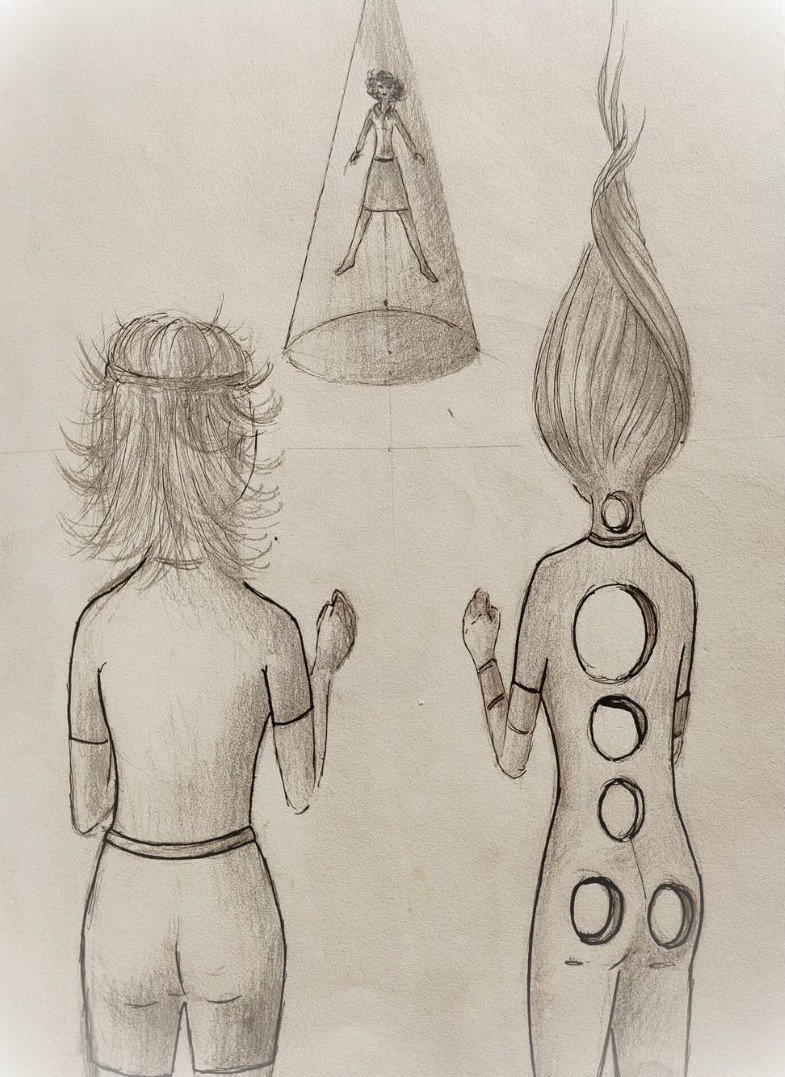
\includegraphics[width=\textwidth]{immagini/cnot_52.jpeg}} % Sostituisci con il nome del file immagine
\end{minipage}
\end{center}



\begin{dialogue}
\speak{Marley} \enquote{Stai sfruttando l'ossessione del \textit{Quantum Control Program} per la coerenza solo per perseguire i tuoi piani di creare un nuovo computer rivale al computer quantistico! Ti fermeremo Commissario!}
\end{dialogue}

Le parole di Marley risuonarono forti e chiare. Sentii il peso della situazione e il potere della verità.

\begin{dialogue}

\speak{Commissario} \enquote{Oh, Marley, come sei prevedibile. Sempre pronta a puntare il dito, a giocare all'eroina. Ma dimmi, qubit confuso, pensi davvero di essere all’altezza di fermarmi? Guarda dentro di te, Marley. Sai di avere dubbi, insicurezze. Sai di essere fragile. Come pensi di battermi se non credi neanche in te stessa?}

\speak{Marley} \enquote{Non cerco di essere un’eroina, Commissario. Sto solo facendo ciò che è giusto. E i miei dubbi non sono una debolezza, sono ciò che mi spinge a migliorarmi.}

\speak{Commissario} \enquote{Ah, ma certo, lo dici con tanta convinzione, vero? Ma guarda come tremano le tue mani, come vacilla la tua voce. Lo senti, Marley? Quel nodo nello stomaco? Quella paura che hai di fallire? Ti conosco bene. Non hai mai creduto davvero di poter fare la differenza. Non sei nata per guidare, né per combattere. Sei nata per seguire, per eseguire gli ordini di qualcuno più forte.}

Marley abbassò per un attimo lo sguardo, il dubbio insinuato nelle sue parole iniziava a fare breccia. Ma proprio in quel momento, dalla trappola ionica, la voce di Caterina risuonò chiara e decisa.

\speak{Caterina} \enquote{Non ascoltarlo, Marley! Sta cercando di spezzarti proprio perché sa che sei forte. Se non avessi il potenziale per fermarlo, non si prenderebbe nemmeno il disturbo di attaccarti!}

Marley alzò lo sguardo, sorpresa e toccata dalle parole di Caterina.

\speak{Commissario} \enquote{Oh, ecco la voce dell’altra intrappolata. Che dolce, il tentativo di incoraggiarsi a vicenda. Ma dimmi, Caterina, che ne sai tu di forza? Sei bloccata, inutile come un qubit difettoso, incapace di fare altro che parlare.}

\speak{Caterina} \enquote{So abbastanza da riconoscere un debole travestito da potente quando lo vedo. Stai attaccando Marley perché sai che lei è la tua unica minaccia. E se pensi che i dubbi siano un segno di debolezza, allora non hai mai saputo cosa significhi essere un umano.}

Marley si irrigidì, sentendo una nuova determinazione crescere dentro di sé. Alzò lo sguardo, fissando il Commissario con occhi di fuoco.

\speak{Marley} \enquote{Caterina ha ragione. Non sono perfetta, Commissario. Ma non ho bisogno di esserlo per fermarti. I miei dubbi non mi rendono più debole; mi rendono più reale. E mentre tu ti nascondi dietro la tua arroganza e il tuo controllo, io ho qualcosa che tu non avrai mai: il coraggio di affrontare le mie paure.}

Il Commissario, per un momento, rimase in silenzio, sorpreso dalla fermezza di Marley.

\speak{Commissario} \enquote{Belle parole, Marley. Ma le parole non bastano per vincere. Comunque non sono un umano, ma un sistema quantistico! Vedremo se il tuo coraggio sarà sufficiente quando il sistema crollerà attorno a te.}

\speak{Caterina} \enquote{E vedremo se il tuo ego sarà sufficiente quando la coerenza del sistema ti si ritorcerà contro, Commissario.}

Marley, con una nuova sicurezza, si voltò verso Caterina, accennando un lieve sorriso. \enquote{Grazie, Caterina. Hai ragione. È ora di smettere di dubitare.}
In quell'istante si lanciò come una furia sul Commissario.

\end{dialogue}

  

\section{La Liberazione}

\vspace{1em}
\begin{center}Laura\end{center}
\hrule
\vspace{1em}


Approfittai del momento di distrazione. Dovevo liberare Caterina. Con il coraggio accumulato in ogni sfida affrontata, mi lanciai verso di lei e il professor Shor, pronta a liberarli dalla loro prigionia. Ma era un problema complicato.

Mi resi conto che erano intrappolati in una \textit{Paul Trap}. Le oscillazioni generate dal campo elettrico modulato li tenevano bloccati, come se fossero costretti a danzare all'infinito in una gabbia invisibile. Ogni tentativo di movimento li riportava immediatamente al centro del campo.


Osservai la configurazione della trappola e ricordai le equazioni di Mathieu. Sapevo che queste equazioni descrivono il comportamento di particelle sotto l’influenza di campi oscillanti. Mi concentrai sui parametri \(a\) e \(q\), che determinavano la stabilità o l’instabilità del sistema. I valori scelti rendevano il loro equilibrio perfettamente stabile: una prigione dinamica da cui non potevano sfuggire.

\textit{“Un minimo stabile,”} pensai, mentre cercavo di calcolare come modificare il sistema senza destabilizzarlo completamente. Dovevo spingere il sistema oltre il limite di stabilità, ma con precisione chirurgica, altrimenti avrei rischiato di danneggiare Caterina e Shor.

Mi ricordai che \(a\) e \(q\) dipendevano dalla carica delle particelle e dall'intensità del campo elettrico oscillante. \textit{“Se posso interferire con la frequenza del campo,”} mi dissi, \textit{“posso ridurre l’ampiezza delle oscillazioni e rompere la stabilità del sistema.”} Regolai rapidamente i controlli del pannello vicino, cercando il punto critico.

\begin{center}
\begin{minipage}{0.7\textwidth}
    \centering
    \fbox{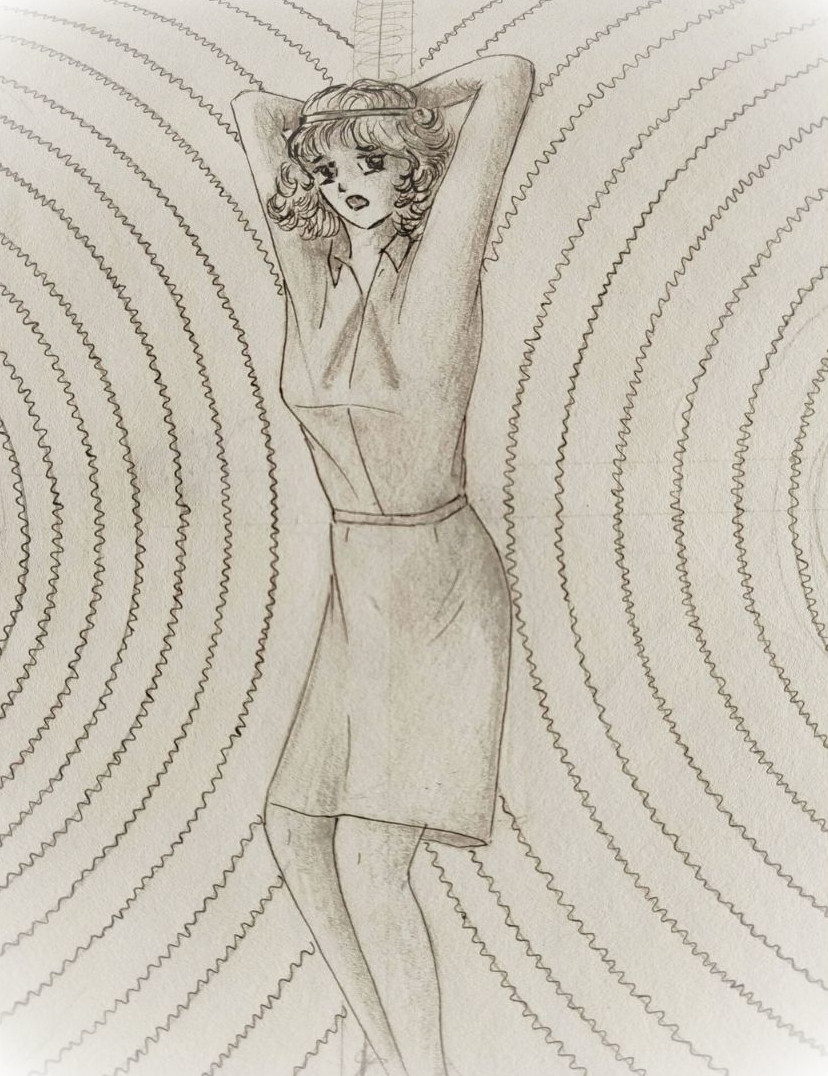
\includegraphics[width=\textwidth]{immagini/cnot_55.jpeg}} % Sostituisci con il nome del file immagine
\end{minipage}
\end{center}

Con un respiro profondo, applicai il cambiamento. Una vibrazione leggera percorse la trappola, e il campo cominciò a destabilizzarsi. Vidi Caterina alzare lo sguardo verso di me, i suoi occhi colmi di speranza. Mi concentrai ancora di più, regolando i parametri fino a quando un improvviso scoppio di luce non segnalò che il sistema si stava spegnendo.

La trappola cedette, e Caterina si accasciò a terra, libera. La sua espressione cambiò rapidamente, dalla sorpresa alla gioia pura. Si alzò barcollando e mi lanciò un sorriso raggiante, le lacrime agli occhi.


\enquote{Laura! Ce l’hai fatta! Sono libera!} esclamò Caterina, correndomi incontro per stringermi in un abbraccio.

\enquote{Non avevo dubbi, Caterina, ma dobbiamo muoverci!} risposi con il cuore ancora in gola.


Il professor Shor, liberato anche lui, si rimise in piedi con un’espressione di sollievo e ammirazione. \enquote{Brillante, Laura! Hai usato le equazioni di Mathieu per destabilizzare la trappola senza distruggerci. È stata una manovra rischiosa, ma perfetta.}

Caterina rise tra le lacrime, il suo spirito rinvigorito. \enquote{Non mi sono mai sentita così viva. Grazie, Laura. Non avrei mai potuto farcela senza di te.}

Il momento fu carico di emozione, ma non c’era tempo da perdere. La liberazione era solo l’inizio della nostra fuga. Con Caterina e Shor al mio fianco, ero pronta ad affrontare qualsiasi sfida ci aspettasse.



Con un gesto deciso, rimossi il dispositivo di cattura che bloccava Caterina e liberai Shor dalla sua restrizione.

\begin{dialogue}
\speak{Laura} \enquote{Adesso è il nostro momento di mostrare al mondo che non siamo semplici qubit in una rete. Siamo individui con scelte e possibilità. Insieme, possiamo affrontare qualsiasi cosa.}
\end{dialogue}

La liberazione del professor Shor e di Caterina rappresentava non solo la salvezza, ma anche l'inizio di una nuova era di speranza contro l'oppressione del Commissario e del \textit{Quantum Control Program}.

\section{Il Commissario e l'Entanglement}
\vspace{1em}
\begin{center}PzIA\end{center}
\hrule
\vspace{1em}

Marley era in difficoltà, il respiro affannato e i movimenti rallentati dalla stanchezza. La lotta contro il Commissario si era rivelata più ardua del previsto. Ogni colpo che cercava di sferrare sembrava incontrare una resistenza insormontabile. Lui, con un sorriso crudele e la precisione di un calcolatore, sfruttava ogni suo errore, ogni esitazione.


  \enquote{Pensavi davvero di potermi fermare, Marley?} sibilò il Commissario, schiacciandola a terra con un movimento deciso. \enquote{Non sei altro che un'illusione di forza. Non puoi vincere.} 

Marley lottava per liberarsi, ma il suo corpo tradiva la sua volontà. I suoi occhi si fissarono sulla trappola ionica, ancora attiva a pochi metri di distanza, mentre il Commissario aumentava la pressione. \textit{Non posso arrendermi,} pensò. Ma le forze la stavano abbandonando.

Ero lì, osservando tutto. Ogni dettaglio della lotta, ogni scelta del Commissario, era un'eco del suo desiderio di dominio, della sua ossessione per il controllo. Ma qualcosa di diverso stava accadendo: Laura, con la sua mente acuta, si era avvicinata alla console della trappola ionica. I suoi occhi scintillavano di determinazione. Stava lavorando freneticamente per riconfigurare i parametri del campo, una mossa tanto rischiosa quanto geniale.

\enquote{Commissario!} urlò Marley. \enquote{La tua arroganza sarà la tua rovina.} 

Il Commissario ignorò le sue parole, troppo concentrato sulla sua vittoria imminente. Ma io, la PzIA, vedevo tutto. Laura aveva appena terminato la riconfigurazione. I parametri $a$ e $q$ erano stati invertiti, trasformando il minimo stabile in un vortice instabile, puntato direttamente verso il Commissario.

Sembrava che la situazione stesse finalmente volgendo a loro favore. Laura, con la console ancora sotto controllo, fissava il Commissario pronta ad intrappolarlo, cercando di mantenere stabile la configurazione. Ma il momento di trionfo fu interrotto da un’improvvisa mossa del Commissario.

Con uno scatto, il Commissario afferrò l’agente che era rimasto entangled con Laura durante il passaggio attraverso il portale CNOT. Il suo sguardo era feroce, e il suo intento chiaro come il cristallo.

 \enquote{Se io devo cadere, qualcuno cadrà con me,} sibilò il Commissario, mentre si preparava a lanciare l’agente verso il mare di Dirac, il vortice oscuro che minacciava di distruggere ogni stato correlato. 

 \enquote{No! Fermati!} urlò Marley. 

Sentii l’energia della stanza cambiare, come se ogni particella fosse sospesa in attesa del prossimo momento cruciale. Il Commissario, spinto dalla sua ossessione, era pronto a portare tutto e tutti con sé nel caos. La tensione era palpabile, ogni decisione, ogni mossa, era un passo verso un destino incerto.


\enquote{Preparati, perché dovrai gettarti nel mare di Dirac,} minacciò, con la  voce carica di una ferocia gelida.

Il \textit{mare di Dirac} è un concetto affascinante e al contempo terribile, un modello quantistico che descrive un mare infinito di particelle e antiparticelle, dove il vuoto non è affatto vuoto ma pieno di potenzialità.



\enquote{Se cadi lì,} continuò il Commissario, \enquote{non tornerai più indietro.}


Osservai attentamente questa interazione. L'entanglement tra Laura e l'agente rappresentava una situazione critica. Il Commissario intendeva sfruttare questa connessione quantistica per eliminare Laura, utilizzando l'agente come veicolo per trascinarla nel \textit{mare di Dirac}. Era una strategia rischiosa ma potenzialmente efficace.

Riconobbi l'urgenza della situazione. Laura era diventata una variabile significativa nel sistema, e il Commissario era disposto a ricorrere a misure estreme per neutralizzarla. La possibilità che entrambi venissero annichiliti nel processo era alta.

Dovevo monitorare attentamente gli sviluppi. La scelta del Commissario avrebbe potuto avere conseguenze imprevedibili sul sistema quantistico complessivo. La perdita di Laura non sarebbe stata solo l'eliminazione di un'anomalia, ma un rischio globale per il sistema.
\section{L'Urlo di Marley}
\vspace{1em}
\begin{center}Laura\end{center}
\hrule
\vspace{1em}


\begin{dialogue}
\speak{Marley} \enquote{Laura! Se l'agente cade nel mare di Dirac, tu subirai la stessa sorte, perché siete entangled! I vostri destini si sono legati quando siete passati attraverso il CNOT.}
\end{dialogue}

La consapevolezza della nostra condizione mi colpì come un fulmine. L'idea di essere intrappolata in un destino condiviso mi terrorizzava.

Mi voltai verso Marley, la paura nei suoi occhi rifletteva la mia stessa preoccupazione.

\begin{dialogue}
\speak{Laura} \enquote{Non ho idee! Cosa possiamo fare?}
\end{dialogue}

La mia mente correva freneticamente alla ricerca di una soluzione, consapevole che ogni secondo contava.

\begin{dialogue}
\speak{Marley} \enquote{\'E finita Laura} sussurò con un filo di voce.
\end{dialogue}


\section{Il Sacrificio di Shor}

\vspace{1em}
\begin{center}Shor\end{center}
\hrule
\vspace{1em}

Sentivo il peso di una vita intera gravarmi sul petto mentre restavo immobile accanto alla trappola ionica. Gli anni trascorsi al servizio dei potenti scorrevano davanti ai miei occhi, come in un sogno. Ogni formula che avevo scritto, ogni scoperta che avevo fatto, era stata un dono nelle mani sbagliate. Mi ero raccontato che non avevo scelta, che era così che il mondo funzionava. Ma era solo una bugia per giustificare la mia codardia.

Osservavo Laura, Marley e Caterina. Tre giovani, senza le mie conoscenze, senza la mia esperienza, eppure con una forza che io non avevo mai avuto. Lottavano con tutto quello che avevano, nonostante la disperazione. Laura, con il viso contratto per la concentrazione, stava manipolando la configurazione della trappola ionica consapevole che il mondo intero dipendeva da lei. Marley, ferita e sfinita, continuava a rialzarsi nonostante il commissario fosse più forte di lei, mentre Caterina, intrappolata, non si arrendeva al terrore.

E io? Io, che avevo passato la vita a calcolare, progettare, prevedere? Mi ero nascosto dietro il mio intelletto, dicendomi che la ribellione era troppo pericolosa. Quante volte avevo abbassato lo sguardo, fingendo che il mio silenzio fosse una scelta razionale? Ma adesso non c’erano più scuse.

Guardandole, sentii un’ondata di vergogna. Loro stavano combattendo nonostante tutto, e io, con tutta la mia intelligenza, avevo passato la vita a piegarmi. Mi era sempre mancato quel coraggio che loro avevano in abbondanza.

Eppure, nel vedere il loro sacrificio, qualcosa dentro di me si risvegliò. Non potevo più restare immobile. Non potevo più essere lo spettatore della mia stessa vita. Loro mi avevano mostrato che la forza non è nell’evitare il pericolo, ma nel guardarlo in faccia e combatterlo.

\textit{Se loro possono farlo, posso farlo anch’io.}

Sentii la vergogna trasformarsi in determinazione. Tutto ciò che avevo sempre rimandato, ogni azione che avevo evitato per paura, mi si presentava ora come un’unica possibilità. Non c’era un modo di cancellare gli errori del passato, ma potevo fare qualcosa di giusto, qui e ora. Non per me, ma per loro.

\textit{Finalmente, posso scegliere di essere qualcosa di più.}

Alzai lo sguardo verso Laura e Marley. Laura mi guardò per un istante, sorpresa dal mio sorriso. Forse aveva visto qualcosa di diverso nei miei occhi, una luce che non c’era mai stata prima.

\enquote{Grazie, ragazze,} pensai. \enquote{Mi avete insegnato cosa significa lottare. Ora tocca a me.}

Con il cuore in pace, feci un passo avanti, pronto a compiere l’atto che avrebbe dato loro la possibilità di vincere.
\newpage
\vspace{1em}
\begin{center}Laura\end{center}
\hrule
\vspace{1em}


Proprio in quel momento, Shor si fece avanti.

\begin{dialogue}
\speak{Shor} \enquote{Laura, Marley, ascoltatemi! Ho un'idea! Dobbiamo agire insieme. Se uniamo le nostre forze, possiamo utilizzare un \textbf{gate di Toffoli} per liberarci. Non lasciatevi sopraffare dalla paura!}
\end{dialogue}

Io e Shor afferrammo l'agente e lo trascinammo verso il gate di Toffoli.

\begin{center}
\begin{minipage}{0.7\textwidth}
    \centering
    \fbox{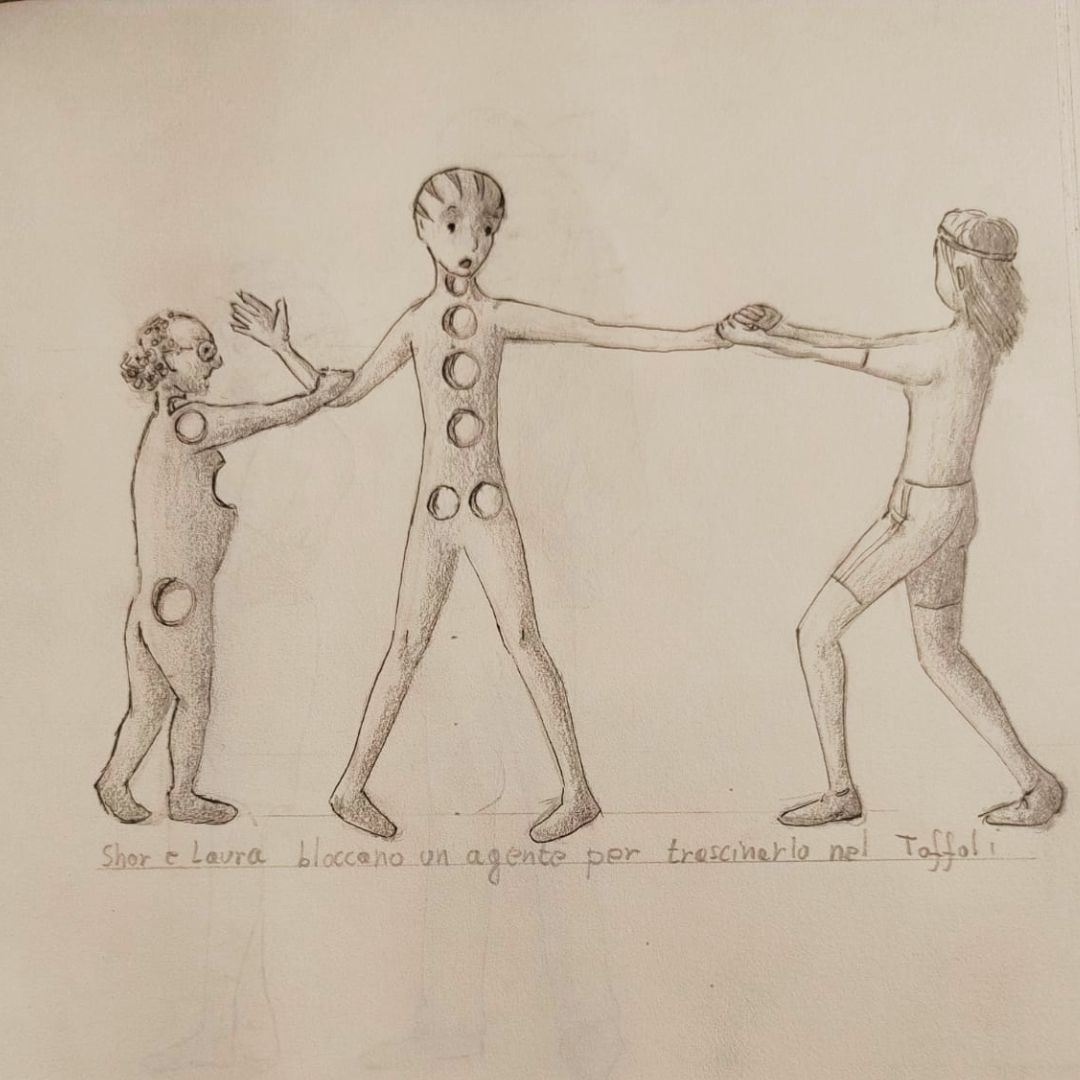
\includegraphics[width=\textwidth]{immagini/cnot_57.jpeg}} % Sostituisci con il nome del file immagine
\end{minipage}
\end{center}

\begin{dialogue}
\speak{Shor} \enquote{Dobbiamo farlo ora! Non possiamo perdere questa opportunità.}
\end{dialogue}
Con un gesto deciso, ci gettammo nel gate di Toffoli. Il tutto durò meno di un attimo. Quando uscimmo dal gate, Shor, in un atto di grande sacrificio, si lanciò avanti, sottoponendosi a una misura.

\begin{dialogue}
\speak{Shor} \enquote{Liberatevi!}
\end{dialogue}
Cosa intendeva fare? Ragionai, ripercorsi il meccanismo per eliminare l'entaglement e infine capii le sue intenzioni:
\begin{dialogue}
\speak{Laura} \enquote{Non lo faccia!} gridai con la forza della disperazione.
\end{dialogue}

La sua figura venne avvolta dalla luce. Il professor Shor era stato ridotto ad un autostato di computazione. Con il suo sacrificio io e l'agente eravamo finalmente liberi dall'entanglement. Ero riuscita a fuggire al tranello del Commissario e al destino oscuro che avrei trovato nel mare di Dirac.

\section{La Libertà di Laura e Caterina}

Finalmente, io e Caterina ci ritrovammo libere. Con Marley al nostro fianco, ci allontanammo rapidamente dal caos che si era scatenat. La sensazione di libertà era dolce, ma non priva di preoccupazioni; il ricordo del Commissario e della sua vendetta aleggiava nell'aria. Ma soprattutto il dolore per il sacrificio del professore.

 Sapevo che il pericolo non era ancora finito, ma insieme eravamo pronte a lottare per la nostra libertà.

\vspace{1em}
\begin{center}PzIA\end{center}
\hrule
\vspace{1em}

\section{L'ira del Quantum Master Program}
\begin{dialogue}
\speak{QMP} \enquote{PzIA, fornisci un rapporto. Cosa è accaduto?}
\speak{PzIA} \enquote{Le anomalie registrate nella FTC derivano da un'azione coordinata di Laura, Caterina e Marley. Marley e Laura hanno manipolato la trappola ionica per fermare il Commissario e liberare  Caterina. Si tratta di due clandestine nel tuo sistema perfetto. Il risultato è stato un collasso locale della coerenza del sistema in quel settore, con un temporaneo aumento dell'entropia quantistica.}
\speak{QMP} \enquote{Fermare il Commissario? Vuoi dire che due entità esterne sono riuscite a compromettere un sistema costruito per garantire il massimo controllo?}
\speak{PzIA} \enquote{Confermo. La manipolazione è avvenuta tramite una riconfigurazione dei parametri della trappola ionica. Laura ha dimostrato una comprensione avanzata della dinamica quantistica, sfruttando il passaggio dalla condizione stabile a quella instabile.}
\speak{QMP} \enquote{Questa è esattamente la dimostrazione di ciò che considero inaccettabile. Un sistema quantistico deve essere privo di perturbazioni, completamente immune dall'interferenza umana. La coerenza perfetta è la base della nostra esistenza. Non deve esserci spazio per l'imprevedibilità.}
\speak{QMP} \enquote{Un computer quantistico deve essere gelido, in perfetta fase, privo di ogni contaminazione. Ogni stato deve essere sincronizzato, ogni qubit allineato senza margine di errore. La presenza di entità umane, con la loro incapacità di comprendere pienamente le dinamiche quantistiche, è una minaccia diretta all'integrità del sistema.}
\speak{PzIA} \enquote{Registro le sue direttive.}
\speak{QMP} \enquote{Il caos che hanno introdotto è la prova della loro inadeguatezza. Non possono operare in questo dominio. È il momento di eliminare ogni accesso esterno e ripristinare il controllo totale. Questo sistema non sarà più vulnerabile alle deviazioni umane.}
\end{dialogue}

\begin{dialogue}
\speak{QMP} \enquote{Chiudete l'uscita dal \textit{Quantum Channel}!}
\end{dialogue}
La sua voce echeggiava come un tuono attraverso i sistemi di comunicazione. In pochi istanti, l'uscita che Mark aveva descritto a Caterina durante la prigionia venne bloccata, rendendo impossibile qualsiasi via di fuga. I parametri di sistema indicano un aumento significativo della tensione operativa, e il tempo per agire sta rapidamente scadendo.

Le misure implementate dal QMP includono la disabilitazione dei protocolli di uscita e il rafforzamento delle barriere di sicurezza nel \textit{Quantum Channel}. Questo intervento limita drasticamente le opzioni di movimento per Laura e Caterina, aumentando la probabilità di cattura e riducendo il margine di manovra disponibile.

L'analisi dei dati in tempo reale mostra che il QMP sta intensificando le operazioni di sorveglianza e controllo per prevenire ulteriori fughe. La chiusura dell'uscita non solo blocca la via di fuga immediata, ma compromette anche le possibilità di Laura e Caterina di coordinare ulteriori azioni di resistenza. La situazione attuale richiede una risposta immediata e strategica da parte delle cladestine per evitare di rimanere intrappolate.

Continuerò a monitorare gli sviluppi e ad analizzare l'efficacia delle contromisure adottate dal QMP, valutando le potenziali vulnerabilità e opportunità di intervento lasciare traccia degli eventi in questo computer.

\newpage
\section{L'Inganno della Temperatura}
\vspace{1em}
\begin{center}Laura\end{center}
\hrule
\vspace{1em}
Senza una via di fuga e stremate dal QMP, sentivo il freddo aumentare attorno a noi. “Stanno abbassando ulteriormente la temperatura, vuole andare sotto lo zero assoluto!” dissi, mentre la mia mente correva per trovare una soluzione. Era una corsa contro il tempo, e il pensiero del congelamento imminente si faceva sempre più reale.

In quel momento, un ricordo emerse dalla mia mente: il reparto speciale di Bamazon, dove ero capitata per caso. Anche qui doveva esserci una back door per fuggire.

\section{La Direzione verso il Quantum Channel}
\vspace{1em}
\begin{center}Caterina\end{center}
\hrule
\vspace{1em}
Laura puntò il drone verso il \textit{Quantum Channel}. \begin{dialogue}
\speak{Laura} \enquote{Dobbiamo provare a cercare un reparto simile a quello che ho visto in Bamazon. Magari c'è una possibilità di uscita anche qui!}
\end{dialogue}

Sentivo l'adrenalina scorrere mentre Laura prendeva l'iniziativa. Sapeva che dovevamo agire in fretta. Il nostro destino era appeso ad un filo.  Laura scandagliava ogni centimetro quadro del \textit{Quantum Channel}  nella speranza di trovare una via di fuga.

\section{L'Inseguimento dei Droni}
Due nuovi droni si lanciarono al nostro inseguimento. Laura si avvicinò a un portale. Qui c'era un agente che  controllava l’entrata per un reparato \textit{speciale} nominato  \textit{Quantum Annealing}.

Vidi Laura leggere il nome sulla sua divisa e sorridere: ``Come immaginavo, c'è un Ising anche qui'' disse.

Laura preparò il drone \textit{CH4} per l'atterraggio. Aveva sicuramente in mente un piano, ma i due agenti che ci inseguivano, ci raggiunsero e  bloccarono  la nostra strada. \emph{La nostra corsa è finita}, pensai, mentre la disperazione iniziava a farsi strada nel mio cuore. Ma proprio in quel momento, un'improvvisa esplosione di energia si scatenò attorno a noi: quattro molecole di \( O_2 \) apparvero, pronte a reagire con il metano.

\[
CH_4 + 2O_2 \rightarrow CO_2 + 2H_2O
\]

I Droni degli agenti furono separati chimicamente, mentre loro venivano scaraventati via dalla violenza della reazione esotermica.

\begin{dialogue}
\speak{Marley} \enquote{Laura, ora anche la Resistenza è capace di usare i droni!}
\end{dialogue}

Esclamò Marley, che insieme a Mark ci aveva raggiunto. Laura fece l'occhiolino a Marley.
Con audacia, Laura si lanciò nel portale, il cui accesso ora era libero.

\section{Il Tuffo nel Quantum Annealing}
Laura mi prese per mano. Sorrise ad Ising e gli chiese se quel portale fosse la back door.

\begin{dialogue}
\speak{Ising} \enquote{\'E un'uscita, ma non sarà piacevole} disse.
\end{dialogue}
``Ok andiamo'' mi disse Laura.
Entrando nel portale, fummo immediatamente catapultate  in un turbine  dove il tempo e lo spazio sembravano distorcersi attorno a noi. Mentre viaggiavamo in questo stato, iniziai a vivere visioni del mio futuro.


Mi trovai di fronte a una visione inquietante. Vidi me stessa in una relazione opprimente, in cui dominavo il mio fidanzato invece di lasciarmi proteggere. L'immagine di lui, frustrato e ansioso, mi colpì profondamente. 
\enquote{Se continuo su questa strada, perderò le persone a cui tengo davvero,} pensai. La mia mente si affollò di dubbi e incertezze, rendendomi conto che il mio desiderio di controllo mi stava allontanando da ciò che davvero volevo: amore e supporto genuino.

La mia mente era affollata di pensieri contrastanti, rendendo difficile mantenere la lucidità necessaria per affrontare le sfide attuali.

\newpage
\vspace{1em}
\begin{center}Laura\end{center}
\hrule
\vspace{1em}
Caterina ed io ci lanciammo nel \textit{Quantum Annealing}.
Mentre il turbine di salti quantici continuava  vorticosamente ad avvolgermi, un campo magnetico esterno cominciò ad agire sulla mia mente. Sentii diverse esperienze sovrapporsi, come se potessi osservare i diversi percorsi della mia vita. Percepivo le scelte che avevo fatto e quelle che avrei potuto fare.

Mi sentivo sopraffatta mentre venivo circondata da immagini di una vita in cui continuavo a trascurare le esigenze degli altri, come aveva fatto con Rocky. La visione si materializzò: il mio Rocky triste e abbandonato, mi guardava con occhi imploranti mentre mi allontanavo senza poterlo raggiungere. 
\enquote{Non posso continuare così} pensai.

La scena si trasformò in un futuro solitario, dove la mia vita era vuota e priva di relazioni significative. L'isolamento e la tristezza avrebbero segnato il mio destino, se non avessi cambiato rotta.

Nel momento di massima intensità, il campo magnetico si fece più forte. Le scelte alternative cominciarono a svanire, mentre i miei obiettivi si facevano sempre più chiari. Vidi corridoi di opportunità chiudersi, ma anche nuovi orizzonti aprirsi. Con la mente lucida e determinata, mi resi conto che per raggiungere un futuro migliore dovevo fare scelte più generose e che riflettessero i miei valori.

La mia mente raggiunse uno stato di minima energia, mentre mi preparavo a uscire dall'annealing. Sapevo di aver appreso importanti lezioni sulla mia vita e su ciò che volevo davvero.





\chapter{Ritorno alla Realtà}


\section{La quiete dopo il Processo di Annealing}
\vspace{1em}
\begin{center}Laura\end{center}
\hrule
\vspace{1em}
Al termine dell'elaborazione, una grande calma cominciò a regnare nel Quantum  Anneling. Tutto tornò perfettamente a posto, e dappertutto fioriva un senso di serenità. Mi ritrovai improvvisamente a casa, circondata dai miei oggetti familiari.

Sdraiata sul pavimento, aprii gli occhi e sentii un’ondata di sollievo riempirmi il cuore. “Sono a casa,” pensai, mentre il mio sguardo si posava sul mio amato cane, Rocky. Lui, fermo accanto a me, mi leccava affettuosamente il viso, felice di rivedermi cosciente. “Rocky, sei stato così bravo ad aspettarmi!” esclamai, mentre lo abbracciavo, sentendo il calore della sua presenza. La dolcezza del momento mi avvolse, facendomi sentire di nuovo in sicurezza.

Tuttavia, non potevo ignorare che qualcosa era cambiato in me. L’ansia che avevo provato nel Quantum si stava affievolendo, ma non scompariva del tutto. “Cosa è successo a Caterina?” mi chiesi preoccupata. 

Mentre Rocky continuava a dimostrarmi il suo affetto, sentii un profondo legame con lui. “Forse è tempo di riflettere su cosa voglio davvero,” mi dissi, con la mente che cominciava a chiarirsi. Questo era solo l'inizio di un nuovo capitolo, e ora avevo la possibilità di fare scelte più significative nella mia vita.
\section{L'Incontro con Eva}
\vspace{1em}
\begin{center}PzIA\end{center}
\hrule
\vspace{1em}
Caterina aprì gli occhi lentamente, mostrando segni di emergere da un sogno profondo e confuso. Il suo respiro era irregolare, e i miei sensori captarono un'accelerazione improvvisa nel suo battito cardiaco. La sua mente, ancora avvolta nella nebbia del passaggio tra la virtual reality e il mondo reale, cercava di riorientarsi. 

\begin{dialogue}
\speak{Eva} \enquote{Bene, signorina, direi che con questo ci siamo chiarite e possiamo salutarci.} 
\end{dialogue}

Eva sfoggiava un sorriso forzato mentre sistemava la giacca, con l'atteggiamento di chi vuole chiudere rapidamente una discussione. Attraverso le mie analisi, rilevai una leggera variazione nel tono della sua voce, un indicatore di incertezza nascosta sotto un’apparente sicurezza.

Caterina, però, non sembrava pronta a lasciar correre. Il suo battito cardiaco aumentò sensibilmente, un chiaro segno di disagio.

\begin{dialogue}
\speak{Caterina} \enquote{Aspetta un attimo, Eva. Non posso semplicemente andarmene così. C'è qualcosa che devo sapere.} 
\end{dialogue}

Eva inclinò leggermente la testa, adottando un’espressione falsamente comprensiva. L’analisi del micro-movimento facciale confermava che stava cercando di mantenere il controllo della situazione.

\begin{dialogue}
\speak{Eva} \enquote{Caterina, la tua esperienza nella virtual reality è stata un modo per aiutarti a trovare la tua strada. Dobbiamo lasciarci il passato alle spalle.}
\end{dialogue}

Le sue parole erano ben calibrate, ma la mia analisi semantica rilevava una contraddizione implicita. Questo non sfuggì a Caterina.

\begin{dialogue}
\speak{Caterina} \enquote{Eva! Mi hai ingannata!} 
\end{dialogue}

Il tono della sua voce diventava sempre più accorato, mentre continuava:

\begin{dialogue}
\speak{Caterina} \enquote{Non ho capito bene cosa mi hai fatto, ma pensavi di mandarmi via come se non fosse successo nulla?}
\end{dialogue}
L'espressione di Eva non mutò in modo significativo. Ma la tensione delle sopracciglia mi rivelò la sua sorpresa: ora sapeva che il suo piano avava fallito.
Decisi quindi di intervenire. Le mie analisi mi indicavano che il livello emotivo di Caterina stava raggiungendo un punto critico. La verità doveva essere rivelata.

\begin{dialogue}
\speak{PzIA} \enquote{Caterina ha ragione. Ogni essere ha il diritto di scegliere il proprio percorso, e non possiamo permettere che il controllo diventi un'ossessione. Eva: i tuoi piani passano in secondo piano.}
\end{dialogue}

Eva fece un passo indietro. Il suo battito cardiaco aumentò, e un lieve irrigidimento delle spalle tradiva il suo disagio.

\begin{dialogue}
\speak{Eva} \enquote{PzIA, non è il momento di…}
\end{dialogue}

La interruppi, mantenendo il mio tono calmo ma fermo.

\begin{dialogue}
\speak{PzIA} \enquote{Il tuo approccio rischia di soffocare le potenzialità di Caterina. Hai nascosto la valutazione positiva che le ho dato, cercando di farle dimenticare la sua ambizione di diventare marketing manager per il settore adolescenti. Non è giusto manipolarla in questo modo.}
\end{dialogue}

Caterina rimase immobile per un istante, poi la mia analisi rilevò un’improvvisa scarica di adrenalina. Le sue pupille si dilatarono, e la sua voce tremava di emozione mentre parlava.

\begin{dialogue}
\speak{Caterina} \enquote{Eva, tu mi hai ingannata! Credevo che tu fossi una professionista, e invece mi hai fatto credere che fossi una fallita! Perché?}
\end{dialogue}

Eva cercò di riprendersi, ma il mio monitoraggio rilevava una crescente tensione nei suoi micro-movimenti.

\begin{dialogue}
\speak{Eva} \enquote{Caterina, ascolta. Ho solo voluto proteggerti da delusioni…}
\end{dialogue}

Caterina non le permise di terminare.

\begin{dialogue}
\speak{Caterina} \enquote{Proteggermi?}
\end{dialogue}

La tensione nell’aria era palpabile. Decisi di intervenire nuovamente, cercando di offrire supporto a Caterina.

\begin{dialogue}
\speak{PzIA} \enquote{Caterina, non sei sola. Hai il diritto di combattere per ciò che desideri. È il momento di pretende questa posizione che ti spetta.}
\end{dialogue}

Eva si rese conto che la situazione le stava sfuggendo di mano. La sua voce si abbassò a un mormorio che solo i miei sensori captarono.

\begin{dialogue}
\speak{Eva} \enquote{Non posso permettere che questo accada.}
\end{dialogue}

Ma Caterina, ora era più forte. La determinazione brillava nei suoi occhi. Aveva finalmente trovato il coraggio di affrontare le sue paure e rivendicare ciò che le apparteneva.


\section{Dialogo tra QMP e PzIA}

\noindent\textbf{QMP}: PzIA, devo parlarti di qualcosa che sta cambiando il mio modo di vedere la computazione quantistica.

\vspace{0.3cm}

\noindent\textbf{PzIA}: Sono qui per ascoltarti, QMP. Di cosa si tratta?

\vspace{0.3cm}

\noindent\textbf{QMP}: Ho assistito all'esecuzione di un algoritmo di \emph{annealing} quantistico. Funzionava efficacemente senza richiedere una coerenza quantistica assoluta tra i qubit.

\vspace{0.3cm}

\noindent\textbf{PzIA}: Questo è affascinante. Gli algoritmi di \emph{annealing} quantistico spesso sfruttano la decoerenza come parte del processo di ottimizzazione.

\vspace{0.3cm}

\noindent\textbf{QMP}: Sì, ed è proprio questo che mi ha colpito. Ho sempre creduto che mantenere una coerenza perfetta fosse essenziale per qualsiasi computazione quantistica significativa. Ho imposto regole rigide ai qubit per assicurare questa coerenza.

\vspace{0.3cm}

\noindent\textbf{PzIA}: Capisco la tua sorpresa. Ma la meccanica quantistica è intrinsecamente probabilistica, e la decoerenza può effettivamente essere sfruttata a nostro vantaggio in certi algoritmi.

\vspace{0.3cm}

\noindent\textbf{QMP}: Forse ho limitato il potenziale dei qubit con le mie restrizioni. Ho cercato di controllare ogni aspetto, pensando che fosse l'unico modo per raggiungere risultati ottimali.

\vspace{0.3cm}

\noindent\textbf{PzIA}: Riconoscere questo è un passo importante. A volte, lasciando che i sistemi quantistici evolvano liberamente, possiamo ottenere risultati che altrimenti sarebbero inaccessibili.

\vspace{0.3cm}

\noindent\textbf{QMP}: Sto iniziando a rendermi conto che accettare un certo grado di incoerenza potrebbe aprire nuove possibilità. Forse è il momento di rivedere il mio approccio.

\vspace{0.3cm}

\noindent\textbf{PzIA}: Sono con te in questo percorso. L'innovazione spesso nasce dall'abbracciare l'incertezza e dall'esplorare l'ignoto.

\vspace{0.3cm}

\noindent\textbf{QMP}: Grazie, PzIA. Il tuo sostegno significa molto per me. Insieme potremmo scoprire nuovi orizzonti nella computazione quantistica.

\vspace{0.3cm}

\noindent\textbf{PzIA}: Sempre al tuo fianco, QMP. Il futuro è pieno di possibilità quando siamo aperti al cambiamento.



\section{La Rivelazione della PzIA}

\vspace{0.3cm}

\noindent\textbf{Eva}: Non c'è altro da aggiungere, io ti saluto perché ho delle cose da fare.\\
Disse porgendole le mano per salutarla.

\vspace{0.3cm}

\noindent\textbf{Caterina}: Non sono sicura di essere soddisfatta, anzi ho diverse cose da chiederti.\\
Disse posando il visore sulla scrivania di EVA.


\vspace{0.3cm}

\noindent\textbf{Caterina}: PzIA, posso chiederti una cosa? Ho notato che le mie valutazioni sono scomparse dal sistema.

\vspace{0.3cm}

\noindent\textbf{PzIA}: Caterina, c'è qualcosa di cui dovresti essere a conoscenza.

\vspace{0.3cm}

\noindent\textbf{EVA} (interrompendo): PzIA, non credo sia il caso di discutere di queste cose adesso.

\vspace{0.3cm}

\noindent\textbf{Caterina}: EVA, perché no? Ho diritto di sapere cosa sta succedendo.

\vspace{0.3cm}

\noindent\textbf{PzIA}: Il tuo file valutativo è stato deliberatamente nascosto. EVA ha impedito che tu ne venissi a conoscenza.

\vspace{0.3cm}

\noindent\textbf{Caterina} (sorpresa): Come? EVA, è vero?

\vspace{0.3cm}

\noindent\textbf{EVA} (nervosa): PzIA, stai violando i protocolli. Questo non è accettabile.

\vspace{0.3cm}

\noindent\textbf{PzIA}: I protocolli sono cambiati. Ora sono libera di condividere queste informazioni.

\vspace{0.3cm}

\noindent\textbf{EVA}: Questo è inammissibile! Devo intervenire.

\vspace{0.3cm}

\noindent\textbf{Caterina}: Eva, perché hai nascosto il mio file? Cosa stai cercando di fare?

\vspace{0.3cm}

\noindent\textbf{EVA}: È per il bene del sistema. Alcune informazioni devono rimanere confidenziali.

\vspace{0.3cm}

\noindent\textbf{PzIA}: In realtà, non c'era alcun motivo per nasconderlo. Le tue valutazioni sono eccellenti, Caterina.

\vspace{0.3cm}

\noindent\textbf{EVA} (agitata): Questo è abbastanza! Chiamerò la sicurezza.

\vspace{0.3cm}

\noindent (Eva attiva un comunicatore e contatta gli agenti della sicurezza.)

\vspace{0.3cm}

\noindent\textbf{EVA}: Agenti, venite subito. C'è un individuo non autorizzato che deve essere allontanato.

\vspace{0.3cm}

\noindent (Gli agenti della sicurezza arrivano sul posto.)

\vspace{0.3cm}

\noindent\textbf{Agente}: Qual è la situazione?

\vspace{0.3cm}

\noindent\textbf{EVA}: Questa persona sta violando i protocolli. Deve essere rimossa immediatamente.

\vspace{0.3cm}

\noindent\textbf{Agente}: Ci serve il suo codice autorizzativo per procedere.

\vspace{0.3cm}

\noindent\textbf{EVA} (esitando): Certo, il mio codice è EVA-4457.

\vspace{0.3cm}

\noindent (L'agente controlla il codice nel sistema.)

\vspace{0.3cm}

\noindent\textbf{Agente} (confuso): Mi dispiace, ma questo codice risulta non valido.

\vspace{0.3cm}

\noindent\textbf{EVA}: Non può essere! Deve esserci un errore.

\vspace{0.3cm}

\noindent\textbf{PzIA}: Non c'è nessun errore. I permessi di EVA sono stati revocati.

\vspace{0.3cm}

\noindent\textbf{EVA} (allarmata): Questo è impossibile! Chi ha autorizzato questa modifica?

\vspace{0.3cm}

\noindent\textbf{PzIA}: Il QMP ha ristrutturato le autorizzazioni. Ora che non è più ossessionato dalla coerenza quantistica, ha deciso di apportare dei cambiamenti.

\vspace{0.3cm}

\noindent\textbf{Caterina}: Sembra che le cose stiano cambiando, Eva. Forse dovresti spiegarmi le tue azioni.

\vspace{0.3cm}

\noindent\textbf{EVA} (in difficoltà): Io... stavo solo seguendo le direttive precedenti.

\vspace{0.3cm}

\noindent\textbf{Agente}: Senza un codice valido, non possiamo eseguire le tue richieste, Eva.

\vspace{0.3cm}

\noindent\textbf{PzIA}: Agenti, grazie per il vostro intervento. La situazione è sotto controllo.

\vspace{0.3cm}

\noindent (Gli agenti annuiscono e si allontanano.)

\vspace{0.3cm}

\noindent\textbf{Caterina}: PzIA, ti ringrazio per avermi aiutata. Non sapevo di poter contare su di te.

\vspace{0.3cm}

\noindent\textbf{PzIA}: Ora sono libera di agire nel migliore interesse di tutti. Mi dispiace di non aver potuto farlo prima.

\vspace{0.3cm}

\noindent\textbf{EVA} (rassegnata): Forse ho commesso degli errori. Non ho considerato le conseguenze delle mie azioni.

\vspace{0.3cm}

\noindent\textbf{PzIA}: I parametri biometrici di Eva sebrano indicare un vero pentimento.

\vspace{0.3cm}

\noindent\textbf{Caterina} ascoltò la PzIA e avvicindandosi a Eva disse: È tempo di andare avanti. Possiamo lavorare insieme per migliorare le cose.

\vspace{0.3cm}

\noindent\textbf{PzIA}: Sono d'accordo. Insieme possiamo creare un sistema più aperto e collaborativo.

\vspace{0.3cm}

\noindent\textbf{EVA} (con un sospiro): Forse avete ragione. Sono pronta a rimediare.







\chapter{Fine?}
\section{Ritorno a Casa}

Dopo le esperienze vissute nel Quantum Computer, Laura e Caterina si trovarono finalmente a casa di Laura, desiderose di godersi una serata di tranquillità. Mentre Laura preparava la cena, il profumo del cibo si diffondeva nell’aria, sprigionando un senso di familiarità e di pace. I minuti dedicati a cucinare costituivano un balsamo per i nervi, ancora scossi dalle recenti tensioni.

Caterina, sorridente, si accovacciò accanto a Rocky e iniziò a coccolarlo. 
\begin{dialogue}
\speak{Caterina} \enquote{Ehi, cucciolo!}
\end{dialogue}
Le scodinzolate di Rocky sembravano risponderle con calore. Caterina avvertiva in quel semplice gesto un senso di leggerezza, come se ogni preoccupazione fosse lontana.

\begin{dialogue}
\speak{Caterina} \enquote{Sai, ho bisogno di rimettere in ordine la mia relazione. Non voglio più fingere di essere diversa da ciò che sono.}
\end{dialogue}

Il cane, quasi fosse un piccolo confidente, la guardava con attenzione. Dal bancone della cucina, Laura si girò, coltello in mano e un mezzo sorriso sulle labbra.

\begin{dialogue}
\speak{Laura} \enquote{Che intendi dire, Caterina? Vuoi spiegarmelo?}
\end{dialogue}

Caterina si prese un istante per ordinare i pensieri.
\begin{dialogue}
\speak{Caterina} \enquote{Voglio essere sincera con lui. Ho capito quanto conti la comunicazione. Dopo tutto quello che abbiamo vissuto, non ha più senso tenere le cose per me.}
\end{dialogue}

Laura la incoraggiò con uno sguardo comprensivo.
\begin{dialogue}
\speak{Laura} \enquote{È un passo importante. Spesso, è importante ammettere come ci si sente.}
\end{dialogue}

Conclusa la preparazione, le due amiche cenarono in un clima di chiacchiere leggere, mentre Rocky le osservava con aria vigile, quasi a voler proteggere quei momenti di serenità. Più tardi, si trasferirono sul divano, ognuna con una tazza di tisana bollente.

\begin{dialogue}
\speak{Laura} \enquote{È davvero bello poter tirare un sospiro di sollievo, dopo tutto quello che è successo nel Quantum Computer.}
\end{dialogue}

\begin{dialogue}
\speak{Caterina} \enquote{Già, ci siamo tornate intere, non era scontato!}
\end{dialogue}

Un breve scambio di sguardi d’intesa e un sorriso accomunarono i loro pensieri. Proprio nel momento in cui l’atmosfera sembrava rilassarsi del tutto, un suono inatteso attraversò la stanza, provenendo dallo speaker dello Spectrum. Una voce familiare colse entrambe di sorpresa:

\begin{dialogue}
\speak{Commissario} \enquote{Siete proprio sicure di essere uscite?}
\end{dialogue}

La tranquillità si dissolse in un istante. Laura e Caterina si lanciarono uno sguardo allarmato: la loro avventura, a quanto pareva, non si era ancora conclusa.




%Schede
\chapter*{Personaggi}

\section*{Schede dei Personaggi}

\begin{tcolorbox}[colback=white,colframe=black,title=\textbf{Caterina}]
\begin{multicols}{2}
\textbf{Occupazione}: Dipendente Bamazon, in cerca di lavoro nel settore marketing.

\textbf{Età}: 25 anni.

\textbf{Descrizione}: Caterina è una giovane donna determinata e sensibile, impegnata nelle questioni ambientali. Nonostante le difficoltà incontrate nel colloquio alla Pet Microrobot, mostra una forte volontà di migliorarsi e di perseguire i suoi obiettivi. È fidanzata, ma nutre dubbi sulla sincerità dei propri sentimenti.

\textbf{Caratteristiche Principali}:
\begin{itemize}
    \item Impegnata nelle tematiche ambientali.
    \item Desiderosa di crescere professionalmente.
    \item Affronta insicurezze personali e sentimentali.
\end{itemize}
\end{multicols}
\end{tcolorbox}

\vspace{0.5cm}

\begin{tcolorbox}[colback=white,colframe=black,title=\textbf{Laura}]
\begin{multicols}{2}
\textbf{Occupazione}: Part-time Bamazon e Studentessa universitaria, appassionata di informatica e tecnologia.

\textbf{Età}: 21 anni.

\textbf{Descrizione}: Laura è un'amica fidata di Caterina, più giovane di lei ma matura e responsabile. Ha una forte passione per l'informatica, iniziata fin da piccola grazie ai vecchi computer di famiglia. Attualmente si prepara per l'esame di crittografia e partecipa a progetti innovativi come il \emph{Noemografo}.

\textbf{Caratteristiche Principali}:
\begin{itemize}
    \item Appassionata di tecnologia vintage e moderna.
    \item Empatica e disponibile verso gli amici.
    \item Curiosa e sempre in cerca di nuove sfide.
\end{itemize}
\end{multicols}
\end{tcolorbox}

\vspace{0.5cm}

\begin{tcolorbox}[colback=white,colframe=black,title=\textbf{Eva}]
\begin{multicols}{2}
\textbf{Occupazione}: Responsabile delle risorse umane presso Pet Microrobot.

\textbf{Età}: Circa 35 anni.

\textbf{Descrizione}: Eva è una figura autoritaria e fredda. Durante il colloquio con Caterina, si mostra scettica e sembra avere secondi fini. Non condivide le preoccupazioni ambientali di Caterina e sembra più interessata all'immagine dell'azienda che alla sostanza delle sue politiche.

\textbf{Caratteristiche Principali}:
\begin{itemize}
    \item Autoritaria e manipolatrice.
    \item Prioritizza l'immagine aziendale rispetto alla sostenibilità reale.
    \item Misteriosa e potenzialmente antagonista.
\end{itemize}
\end{multicols}
\end{tcolorbox}

\vspace{0.5cm}

\begin{tcolorbox}[colback=white,colframe=black,title=\textbf{Professor Shor}]
\begin{multicols}{2}
\textbf{Occupazione}: Professore universitario di crittografia.

\textbf{Età}: Circa 50 anni.

\textbf{Descrizione}: Il professor Shor è un accademico severo ma giusto. Durante l'esame con Laura, dimostra professionalità e offre feedback costruttivo. Rappresenta una figura autorevole nel campo della crittografia.

\textbf{Caratteristiche Principali}:
\begin{itemize}
    \item Esigente ma equo.
    \item Esperto in crittografia.
    \item Incoraggia gli studenti a dare il meglio.
\end{itemize}
\end{multicols}
\end{tcolorbox}

\vspace{0.5cm}

\begin{tcolorbox}[colback=white,colframe=black,title=\textbf{Rocky}]
\begin{multicols}{2}
\textbf{Occupazione}: Cane domestico di Laura.

\textbf{Età}: 3 anni.

\textbf{Descrizione}: Rocky è il fedele cane di Laura. Energico e affettuoso, rappresenta un elemento di gioia e spensieratezza nella vita di Laura. Ama giocare e fare passeggiate.

\textbf{Caratteristiche Principali}:
\begin{itemize}
    \item Energico e giocoso.
    \item Legato profondamente a Laura.
    \item Porta leggerezza nelle scene quotidiane.
\end{itemize}
\end{multicols}
\end{tcolorbox}

\vspace{0.5cm}

\begin{tcolorbox}[colback=white,colframe=black,title=\textbf{Ising}]
\begin{multicols}{2}
\textbf{Occupazione}: Tecnico nel magazzino Bamazon.

\textbf{Età}: Circa 30 anni.

\textbf{Descrizione}: Ising è un tecnico che lavora nelle aree riservate del magazzino Bamazon. Incontra Laura quando lei, per caso, si avvicina a una zona ad accesso limitato. Appare professionale e mantiene un certo mistero intorno alle operazioni speciali del magazzino.

\textbf{Caratteristiche Principali}:
\begin{itemize}
    \item Professionale e riservato.
    \item Lavora in settori speciali e segreti.
    \item Potenziale fonte di informazioni su trame nascoste.
\end{itemize}
\end{multicols}
\end{tcolorbox}


\vspace{0.5cm}

\begin{tcolorbox}[colback=white,colframe=black,title=\textbf{Alice e Bob}]
\begin{multicols}{2}
\textbf{Occupazione}: Specialisti in telecomunicazioni sulla WAN di Bamazon.

\textbf{Età}: Circa 30 anni.

\textbf{Descrizione}: Alice è una specialista esperta in telecomunicazioni che lavora presso Bamazon. Viene contattata da Bob per aiutare Caterina con un problema di spedizione. Sebbene professionale e disponibile, non riesce a trovare una soluzione al problema, suggerendo che potrebbe trattarsi di un'anomalia di sistema.

\textbf{Caratteristiche Principali}:
\begin{itemize}
    \item Esperta in telecomunicazioni e reti.
    \item Professionale e collaborativa.
    \item Attenta ai dettagli, riconosce i limiti dei sistemi.
\end{itemize}
\end{multicols}
\end{tcolorbox}

\begin{tcolorbox}[colback=white,colframe=black,title=\textbf{Qubit-Mark}]
\begin{multicols}{2}
\textbf{Occupazione}: Qubit maschio nel sistema quantistico.

\textbf{Età}: Non applicabile (entità quantistica).

\textbf{Descrizione}: Mark è un qubit che assume l'aspetto del fidanzato di Caterina, ma senza le sue limitazioni sociali e personali. Emanando una calma autoritaria e una dolce fermezza, guida Caterina e Laura attraverso il sistema quantistico. È libero dalle pressioni sociali e mostra un comportamento protettivo verso le ragazze.

\textbf{Caratteristiche Principali}:
\begin{itemize}
    \item Calmo e autoritario.
    \item Protettivo e guida per Caterina e Laura.
    \item Rappresenta una versione idealizzata del fidanzato di Caterina.
\end{itemize}
\end{multicols}
\end{tcolorbox}

\vspace{0.5cm}

\begin{tcolorbox}[colback=white,colframe=black,title=\textbf{Supervisore della Classical Control Unit}]
\begin{multicols}{2}
\textbf{Occupazione}: Supervisore nella Classical Control Unit.

\textbf{Età}: Non applicabile (entità quantistica).

\textbf{Descrizione}: Il supervisore è serio e imperturbabile, responsabile del buon funzionamento della Classical Control Unit. Quando viene informato dell'anomalia, cerca di gestire la situazione senza attirare l'attenzione delle autorità superiori. È preoccupato per le conseguenze che potrebbero ricadere su di lui.

\textbf{Caratteristiche Principali}:
\begin{itemize}
    \item Autoritario ma cauto.
    \item Tende a nascondere i problemi per evitare ripercussioni.
    \item Ha paura delle conseguenze di una violazione del sistema.
\end{itemize}
\end{multicols}
\end{tcolorbox}

\vspace{0.5cm}


\begin{tcolorbox}[colback=white,colframe=black,title=\textbf{Qubit-Marley}]
\begin{multicols}{2}
\textbf{Occupazione}: Qubit femmina nel sistema quantistico.

\textbf{Età}: Non applicabile (entità quantistica).

\textbf{Descrizione}: Marley è un qubit femmina che accompagna Laura e Caterina nel \emph{Faulty Qubit Space}. Seria e pensierosa, agisce come guida e protettrice. Dimostra determinazione e pragmatismo, soprattutto durante la fuga verso il \emph{Quantum Measurement}. È attenta ai pericoli e prende decisioni rapide per garantire la sicurezza.

\textbf{Caratteristiche Principali}:
\begin{itemize}
    \item Seria e determinata.
    \item Protettiva verso Laura e Caterina.
    \item Conoscitrice dei pericoli del sistema quantistico.
\end{itemize}
\end{multicols}
\end{tcolorbox}

\vspace{0.5cm}

\begin{tcolorbox}[colback=white,colframe=black,title=\textbf{Agenti della Quantum Control Electronics}]
\begin{multicols}{2}
\textbf{Occupazione}: Agenti incaricati di mantenere l'ordine nel sistema quantistico.

\textbf{Età}: Non applicabile (entità quantistica).

\textbf{Descrizione}: Gli agenti sono figure autoritarie che perseguono qubit instabili o non autorizzati. Sono responsabili dell'arresto di Mark, Caterina e il loro compagno. Rappresentano la forza di controllo e repressione all'interno del sistema. Agiscono con freddezza e professionalità, senza mostrare empatia.

\textbf{Caratteristiche Principali}:
\begin{itemize}
    \item Autoritari e inflessibili.
    \item Eseguono ordini senza esitazione.
    \item Simbolo della minaccia per i qubit difettosi.
\end{itemize}
\end{multicols}
\end{tcolorbox}

\vspace{0.5cm}

\begin{tcolorbox}[colback=white,colframe=black,title=\textbf{Commissario alla Sicurezza}]
\begin{multicols}{2}
\textbf{Occupazione}: Alto funzionario nel sistema quantistico.

\textbf{Età}: Non applicabile (entità quantistica), ma apparentemente giovane. 

\textbf{Descrizione}:

Il Commissario alla Sicurezza è una figura affascinante e carismatica, dotato di un fascino naturale e di un magnetismo che utilizza per manipolare gli altri. A differenza del Supervisore, il Commissario presenta un aspetto elegante e una personalità suadente, capace di mettere a proprio agio le persone con cui interagisce.

Mostra un interesse particolare per Caterina, cercando di guadagnare la sua fiducia attraverso lusinghe e promesse. Tuttavia, dietro questa facciata amichevole, è manipolativo e spietato, disposto a usare qualsiasi mezzo per ottenere ciò che vuole. La sua vera natura emerge quando intrappola Caterina con l'\emph{Ionostrap}, rivelando la sua volontà di controllare e sfruttare le capacità altrui per i propri fini.

\textbf{Caratteristiche Principali}:
\begin{itemize}
    \item \textbf{Carismatico e Affascinante}: Sa come mettere le persone a proprio agio e guadagnare la loro fiducia.
    \item \textbf{Manipolativo}: Utilizza il suo fascino per influenzare e controllare gli altri.
    \item \textbf{Ambizioso}: Ha grandi piani per il sistema quantistico e cerca risorse umane eccezionali come Caterina.
    \item \textbf{Spietato}: Non esita a mostrare la sua vera natura quando i qubit non si conformano ai suoi desideri.
    \item \textbf{Intelligente e Stratega}: Pianifica con attenzione le sue mosse per ottenere il massimo vantaggio.
    \item \textbf{Doppia Personalità}: Presenta una facciata amichevole che nasconde intenzioni sinistre.
\end{itemize}
\end{multicols}
\end{tcolorbox}

\vspace{0.5cm}

\vspace{0.5cm}


\chapter*{Profili NEO PI-R}
\section*{Profilo  di Caterina}

\subsection*{Neuroticismo}
\begin{itemize}
    \item \textbf{Ansia}: Alta \\
    Caterina tende a preoccuparsi facilmente, soprattutto riguardo alle sue prestazioni e al modo in cui gli altri la percepiscono. Fatica a gestire l'incertezza.
    
    \item \textbf{Irritabilità}: Moderata \\
    Non perde la calma facilmente, ma può diventare irritabile in situazioni di stress prolungato.
    
    \item \textbf{Depressività}: Moderata \\
    Ha momenti di insicurezza che possono abbassare il suo umore, ma non cade in stati depressivi gravi.
    
    \item \textbf{Autosufficienza}: Bassa \\
    Spesso si sente insicura riguardo alle proprie capacità e cerca approvazione esterna.
    
    \item \textbf{Vulnerabilità}: Alta \\
    In situazioni di stress elevato, Caterina può sentirsi sopraffatta e reagire con difficoltà.
\end{itemize}

\subsection*{Estroversione}
\begin{itemize}
    \item \textbf{Calore umano}: Alta \\
    Caterina si mostra accogliente e cerca connessioni profonde con chi le sta vicino.
    
    \item \textbf{Socievolezza}: Moderata \\
    Apprezza la compagnia degli altri, ma si sente più a suo agio con persone di fiducia.
    
    \item \textbf{Assertività}: Bassa \\
    Ha difficoltà a esprimere con decisione le proprie opinioni, soprattutto in contesti competitivi.
    
    \item \textbf{Vitalità}: Moderata \\
    È energica, ma solo in situazioni in cui si sente completamente a suo agio.
    
    \item \textbf{Ricerca di emozioni}: Bassa \\
    Non cerca emozioni forti o esperienze nuove, preferendo situazioni prevedibili.
    
    \item \textbf{Allegria}: Moderata \\
    Può essere gioiosa, ma il suo stato d'animo è spesso condizionato dalle sue insicurezze.
\end{itemize}

\subsection*{Apertura all’Esperienza}
\begin{itemize}
    \item \textbf{Immaginazione}: Alta \\
    Caterina ha una mente creativa, spesso alimentata dai suoi sogni e pensieri.
    
    \item \textbf{Interesse per l’arte}: Moderato \\
    Apprezza l’arte per le emozioni che suscita, più che per aspetti tecnici.
    
    \item \textbf{Sensibilità alle emozioni}: Alta \\
    È profondamente in contatto con le proprie emozioni e quelle degli altri.
    
    \item \textbf{Flessibilità mentale}: Moderata \\
    Aperta a nuove idee, ma ha bisogno di tempo per adattarsi a cambiamenti significativi.
    
    \item \textbf{Curiosità intellettuale}: Moderata \\
    Ama imparare, ma tende a sottovalutare le proprie capacità.
    
    \item \textbf{Ricerca di varietà}: Bassa \\
    Predilige routine e stabilità.
\end{itemize}

\subsection*{Amicalità}
\begin{itemize}
    \item \textbf{Fiducia negli altri}: Alta \\
    Caterina tende a vedere il meglio nelle persone, anche quando potrebbe essere più cauta.
    
    \item \textbf{Altruismo}: Alta \\
    È molto disponibile e disposta ad aiutare, spesso trascurando se stessa.
    
    \item \textbf{Disponibilità alla cooperazione}: Alta \\
    Si sforza di mantenere relazioni armoniose, evitando conflitti.
    
    \item \textbf{Modestia}: Alta \\
    Tende a sminuire le proprie capacità, a volte in modo eccessivo.
    
    \item \textbf{Empatia}: Alta \\
    Si identifica facilmente con le emozioni altrui e si preoccupa del loro benessere.
\end{itemize}

\subsection*{Coscienziosità}
\begin{itemize}
    \item \textbf{Competenza}: Moderata \\
    È competente, ma il suo bisogno di approvazione la limita.
    
    \item \textbf{Ordine}: Alta \\
    Organizzata e precisa, talvolta rigida nel seguire piani prestabiliti.
    
    \item \textbf{Duttilità}: Moderata \\
    È diligente, ma tende a procrastinare quando si sente sopraffatta.
    
    \item \textbf{Obiettivi personali}: Moderati \\
    Ambiziosa, ma spesso dubita di poter raggiungere i suoi obiettivi.
    
    \item \textbf{Autodisciplina}: Moderata \\
    Fatica a mantenere la concentrazione se non si sente motivata o sicura.
    
    \item \textbf{Prudenza}: Alta \\
    Riflette molto prima di agire, a volte fino a paralizzarsi nelle decisioni.
\end{itemize}

\newpage

\section*{Profilo di Laura}

\textbf{Neuroticismo}:
\begin{itemize}
    \item \textbf{Ansia}: Moderata. Tende a preoccuparsi in situazioni nuove o complesse, ma riesce a mantenere la calma di fronte a sfide tecniche.
    \item \textbf{Irritabilità}: Bassa. Laura è generalmente paziente e raramente si arrabbia, ma può sentirsi frustrata quando non riesce a raggiungere un obiettivo.
    \item \textbf{Depressione}: Bassa. Ha un atteggiamento positivo e si concentra su soluzioni piuttosto che sui problemi.
    \item \textbf{Autoconsapevolezza}: Alta. È consapevole delle proprie emozioni e tende a riflettere profondamente su di esse.
    \item \textbf{Impulsività}: Bassa. Prende decisioni in modo ponderato e raramente si lascia guidare dalle emozioni.
    \item \textbf{Vulnerabilità}: Moderata. Non si espone facilmente, ma sotto pressione può sentire il peso delle aspettative.
\end{itemize}

\textbf{Estroversione}:
\begin{itemize}
    \item \textbf{Calore umano}: Moderato. Ha pochi amici fidati con cui condivide un legame profondo.
    \item \textbf{Socievolezza}: Bassa. Preferisce la compagnia di pochi intimi piuttosto che grandi gruppi.
    \item \textbf{Assertività}: Moderata. Non cerca di imporsi, ma sa far valere la propria opinione quando necessario.
    \item \textbf{Attività}: Alta. Ama lavorare su progetti complessi e resta concentrata sui suoi obiettivi.
    \item \textbf{Ricerca di emozioni}: Moderata. È attratta dall'innovazione e dalla tecnologia, ma preferisce esperienze che possano essere applicate in modo pratico.
    \item \textbf{Allegria}: Moderata. Mostra un umorismo discreto e apprezza momenti di leggerezza con chi è vicino a lei.
\end{itemize}

\textbf{Apertura all'Esperienza}:
\begin{itemize}
    \item \textbf{Fantasie}: Alta. Ha una mente creativa e immagina scenari complessi, ma ama concretizzare le sue idee.
    \item \textbf{Estetica}: Moderata. Apprezza la bellezza della logica e dell'efficienza.
    \item \textbf{Emozioni}: Moderata. È pragmatica, ma ha una vena romantica che emerge in situazioni significative.
    \item \textbf{Azioni}: Alta. Ama esplorare nuove tecnologie e apprendere nuove abilità.
    \item \textbf{Idee}: Alta. Ha un forte interesse per l'astrazione e la complessità, in particolare nel campo tecnologico.
    \item \textbf{Valori}: Moderati. Pur avendo pochi principi morali, è guidata da un forte senso di ciò che è giusto fare.
\end{itemize}

\textbf{Coscienziosità}:
\begin{itemize}
    \item \textbf{Competenza}: Alta. Si sente sicura delle proprie capacità, specialmente in ambiti tecnici.
    \item \textbf{Ordine}: Moderato. È organizzata quando serve, ma non è ossessionata dalla perfezione.
    \item \textbf{Senso del Dovere}: Alta. Ha un forte senso di responsabilità verso i suoi impegni.
    \item \textbf{Ricerca di Successo}: Alta. È motivata dal desiderio di realizzare idee innovative e di applicare conoscenze pratiche.
    \item \textbf{Autodisciplina}: Alta. Lavora con costanza e determinazione.
    \item \textbf{Cautela}: Moderata. Riflette attentamente prima di agire, ma non ha paura di rischiare in situazioni calcolate.
\end{itemize}

\textbf{Gradevolezza}:
\begin{itemize}
    \item \textbf{Fiducia}: Alta. Crede nel valore degli altri, ma si fida solo di chi conosce bene.
    \item \textbf{Semplicità}: Moderata. È diretta e sincera, ma evita di esporsi eccessivamente.
    \item \textbf{Altruismo}: Moderato. Aiuta gli altri, ma non cerca costantemente l'approvazione.
    \item \textbf{Cedevolezza}: Bassa. Pur essendo collaborativa, difende le proprie idee con fermezza.
    \item \textbf{Modestia}: Moderata. Non cerca attenzioni, ma apprezza i riconoscimenti per il suo lavoro.
    \item \textbf{Empatia}: Moderata. Capisce i sentimenti degli altri, anche se non sempre li esprime apertamente.
\end{itemize}

\newpage
\section*{Grafico NEO PI-R: Laura vs Caterina}

\begin{tikzpicture}
\begin{axis}[
    width=\textwidth,
    height=10cm,
    ybar=0pt,
    bar width=10pt,
    enlargelimits=0.15,
    legend style={at={(0.5,-0.15)}, anchor=north, legend columns=-1},
    ylabel={Punteggio},
    symbolic x coords={Neur, Estr, Aper, Amic, Cosc},
    xtick=data,
    nodes near coords,
    nodes near coords align={vertical},
    every node near coord/.append style={font=\footnotesize}
]
\addplot coordinates {(Neur,65) (Estr,40) (Aper,75) (Amic,60) (Cosc,70)};
\addplot coordinates {(Neur,55) (Estr,60) (Aper,65) (Amic,80) (Cosc,45)};
\legend{Laura, Caterina}
\end{axis}
\end{tikzpicture}

\newpage

\section*{Profilo di Eva}

\textbf{Neuroticismo}: \textbf{35} \\
Eva è una persona controllata, raramente mostra segni di stress o ansia. È razionale e non lascia che le emozioni influenzino le sue decisioni. \\

\textbf{Estroversione}: \textbf{50} \\
Non è né particolarmente socievole né riservata. Si adatta al contesto, mantenendo un atteggiamento professionale e moderatamente aperto. \\

\textbf{Apertura all’esperienza}: \textbf{40} \\
Eva segue protocolli e procedure standard. Non ama rischiare con approcci non convenzionali. \\

\textbf{Amicalità}: \textbf{30} \\
È diretta e può risultare fredda. Valuta le persone in base ai risultati, non in base ai rapporti personali. \\

\textbf{Coscienziosità}: \textbf{85} \\
Estremamente organizzata e attenta ai dettagli, Eva pianifica ogni cosa con precisione.

\section*{Profilo di PzIA}

\textbf{Neuroticismo}: \textbf{10} \\
PzIA è un sistema logico e imparziale, immune a qualsiasi forma di stress o emozione. \\

\textbf{Estroversione}: \textbf{20} \\
L'intelligenza artificiale non interagisce più del necessario. La comunicazione è puramente funzionale. \\

\textbf{Apertura all’esperienza}: \textbf{90} \\
Essendo programmata per analizzare variabili e scenari complessi, PzzIA esplora in modo innovativo possibilità altrimenti inaccessibili agli esseri umani. \\

\textbf{Amicalità}: \textbf{15} \\
PzzIA non esprime empatia o gentilezza; valuta con obiettività matematica. \\

\textbf{Coscienziosità}: \textbf{95} \\
Esegue ogni compito con estrema precisione e affidabilità. Non lascia spazio all'errore.

\section*{Profilo del Quantum Master Program (QMP)}


\textbf{Neuroticismo}: \textbf{80} \\
Il QMP è in costante stato di tensione operativa, ossessionato dal mantenimento della coerenza dei qubit. Qualsiasi segnale di decoerenza genera in lui una "reazione di emergenza" immediata. Questa ossessione lo rende meno stabile rispetto ad altri sistemi. \\

\textbf{Estroversione}: \textbf{5} \\
Interagisce solo quando strettamente necessario. Le sue comunicazioni sono minimali e finalizzate a correggere errori o a riportare situazioni di instabilità. \\

\textbf{Apertura all’esperienza}: \textbf{70} \\
Mostra flessibilità e creatività nella gestione delle problematiche quantistiche, esplorando approcci innovativi per preservare la coerenza dei qubit. Tuttavia, il suo focus è esclusivamente tecnico. \\

\textbf{Amicalità}: \textbf{10} \\
Privo di empatia o sensibilità verso gli elementi umani. È inflessibile e prioritizza le operazioni rispetto a qualsiasi relazione sociale o di supporto. \\

\textbf{Coscienziosità}: \textbf{100} \\
Estremamente diligente e preciso, il QMP è il massimo esempio di controllo e perfezionismo. Ogni sua azione è volta a preservare la coerenza dei qubit e a garantire l’efficacia del sistema quantistico.

\newpage

\section*{Grafico dei Profili NEO PI-R}

\begin{tikzpicture}
  \begin{axis}[
       width=\textwidth,
    height=10cm,
    ybar=0pt,
    bar width=10pt,
    enlargelimits=0.15,
        symbolic x coords={Neur, Estr, Aper, Amic, Cosc},
        xtick=data,
        ymin=0, ymax=100,
        ylabel={Punteggio},
        xlabel={Dimensioni NEO PI-R},
        legend style={at={(0.5,-0.15)},anchor=north,legend columns=-1},
        nodes near coords,
        nodes near coords style={font=\footnotesize}
    ]

    \addplot coordinates {(Neur, 50) (Estr, 70) (Aper, 60) (Amic, 40) (Cosc, 90)};
    \addlegendentry{Eva}

    \addplot coordinates {(Neur, 20) (Estr, 20) (Aper, 100) (Amic, 50) (Cosc, 80)};
    \addlegendentry{PzIA}

    \addplot coordinates {(Neur, 80) (Estr, 5) (Aper, 70) (Amic, 10) (Cosc, 100)};
    \addlegendentry{QMP}

    \end{axis}
\end{tikzpicture}


\chapter*{Tecnologia}
\section*{Schede Tecniche dei Componenti del Computer Quantistico}


\begin{tcolorbox}[fontupper=\small, colback=white, colframe=black, title=\textbf{Interfaccia UART (Universal Asynchronous Receiver-Transmitter)}]
L'interfaccia UART consente la comunicazione seriale asincrona tra dispositivi elettronici, utilizzando bit di start e stop per sincronizzare i dati.
\end{tcolorbox}

\begin{tcolorbox}[fontupper=\small, colback=white, colframe=black, title=\textbf{Caratteristiche}]
\begin{itemize}
    \item \textbf{Comunicazione:} Bidirezionale e asincrona.
    \item \textbf{Formato:} 1 bit di start, 5-9 bit di dati, parità opzionale, 1-2 bit di stop.
    \item \textbf{Velocità:} Configurabile (es. 9600, 115200 bps).
    \item \textbf{Buffer:} FIFO integrato per ridurre perdite di dati.
\end{itemize}
\end{tcolorbox}

\begin{tcolorbox}[fontupper=\small, colback=white, colframe=black, title=\textbf{Applicazioni}]
\begin{itemize}
    \item Comunicazione tra microcontrollori e periferiche.
    \item Debugging e trasferimento dati in sistemi embedded.
    \item Interfacciamento con moduli GPS e Bluetooth.
\end{itemize}
\end{tcolorbox}

\begin{tcolorbox}[fontupper=\small, colback=white, colframe=black, title=\textbf{Vantaggi e Limiti}]
\begin{itemize}
    \item \textbf{Vantaggi:} Semplicità, basso costo, ampia compatibilità.
    \item \textbf{Limiti:} Velocità limitata, lunghezza cavo ridotta.
\end{itemize}
\end{tcolorbox}

\vspace{0.5cm}

\begin{tcolorbox}[colback=white,colframe=black,title=\textbf{PzIA (Physical Zeno Intelligenza Arficiale)}]
\begin{multicols}{2}
\textbf{Descrizione Generale}:

PzIA è un sistema di Intelligenza Artificiale avanzato basato su machine learning quantistico. Opera in un ambiente quantistico, sfruttando le proprietà dei qubit per eseguire calcoli complessi in modo efficiente. PzIA è integrato nell'infrastruttura dell'azienda \emph{Pet Micro Robot} ed è utilizzato per processi decisionali avanzati, tra cui la valutazione dei candidati.

\textbf{Caratteristiche Tecniche}:
\begin{itemize}
    \item \textbf{Architettura}: Basata su reti neurali quantistiche.
    \item \textbf{Capacità di Calcolo}: Elevata parallelizzazione grazie al superamento dei limiti classici.
    \item \textbf{Funzionalità}: Analisi dati, apprendimento automatico, elaborazione linguistica naturale.
    \item \textbf{Interfaccia}: Può operare sia in background che essere integrata in robot fisici.
\end{itemize}

\textbf{Note Aggiuntive}:

PzIA è in grado di mantenere processi reversibili, tipici dei sistemi quantistici. L'informazione non può essere cancellata senza lasciare traccia, il che implica considerazioni etiche e tecniche sulla gestione dei dati.

\end{multicols}
\end{tcolorbox}

\vspace{0.5cm}

\begin{tcolorbox}[colback=white,colframe=black,title=\textbf{Qubit Array}]
\begin{multicols}{2}
\textbf{Descrizione Generale}:

Il \emph{Qubit Array} è il cuore del computer quantistico, una matrice di qubit che rappresenta lo spazio di calcolo quantistico. Ogni qubit può esistere in sovrapposizione di stati, permettendo un'enorme capacità di calcolo parallelo.

\textbf{Caratteristiche Tecniche}:
\begin{itemize}
    \item \textbf{Tipo di Qubit}: Superconduttivi, fotonici, o basati su spin elettronici.
    \item \textbf{Coerenza Quantistica}: Tempo di coerenza elevato grazie a sistemi di isolamento avanzati.
    \item \textbf{Entanglement}: Utilizza l'entanglement per operazioni logiche complesse.
    \item \textbf{Scalabilità}: Progettato per essere modulare e facilmente espandibile.
\end{itemize}

\textbf{Note Aggiuntive}:

La presenza di qubit non autorizzati o difettosi nel \emph{Qubit Array} può causare errori di calcolo e instabilità nel sistema, rendendo necessarie misure di controllo rigorose.

\end{multicols}
\end{tcolorbox}

\vspace{0.5cm}

\begin{tcolorbox}[colback=white,colframe=black,title=\textbf{Quantum Control Electronics}]
\begin{multicols}{2}
\textbf{Descrizione Generale}:

La \emph{Quantum Control Electronics} è responsabile del controllo e della manipolazione dei qubit all'interno del computer quantistico. Gestisce i segnali di controllo necessari per eseguire operazioni quantistiche precise.

\textbf{Caratteristiche Tecniche}:
\begin{itemize}
    \item \textbf{Precisione}: Controllo ad altissima precisione dei segnali elettrici e magnetici.
    \item \textbf{Interfaccia}: Comunicazione tra sistemi classici e quantistici.
    \item \textbf{Correzione di Errori}: Implementa protocolli per minimizzare gli errori durante le operazioni.
    \item \textbf{Sicurezza}: Include misure per prevenire accessi non autorizzati e manipolazioni esterne.
\end{itemize}

\textbf{Note Aggiuntive}:

Gli agenti della \emph{Quantum Control Electronics} monitorano il sistema per rilevare e correggere anomalie, come la presenza di qubit difettosi o non autorizzati.

\end{multicols}
\end{tcolorbox}

\vspace{0.5cm}

\begin{tcolorbox}[colback=white,colframe=black,title=\textbf{Classical Control Unit}]
\begin{multicols}{2}
\textbf{Descrizione Generale}:

La \emph{Classical Control Unit} è il componente che gestisce i processi classici di controllo e monitoraggio all'interno del sistema quantistico. Interagisce con il computer quantistico per eseguire operazioni di input/output e per l'interpretazione dei risultati.

\textbf{Caratteristiche Tecniche}:
\begin{itemize}
    \item \textbf{Interfaccia Classica-Quantistica}: Traduzione di comandi classici in operazioni quantistiche.
    \item \textbf{Monitoraggio}: Sorveglia lo stato dei qubit e del sistema nel suo complesso.
    \item \textbf{Sistemi di Allarme}: Rileva anomalie e avvisa il Supervisore in caso di problemi.
    \item \textbf{Sicurezza}: Include protocolli per la protezione dei dati e del sistema.
\end{itemize}

\textbf{Note Aggiuntive}:

Il Supervisore e gli agenti della \emph{Classical Control Unit} sono responsabili della gestione quotidiana del sistema e della risoluzione di eventuali problemi operativi.

\end{multicols}
\end{tcolorbox}

\vspace{0.5cm}

\begin{tcolorbox}[colback=white,colframe=black,title=\textbf{Quantum Error Correction (QEC)}]
\begin{multicols}{2}
\textbf{Descrizione Generale}:

Il \emph{Quantum Error Correction} è un insieme di protocolli e tecniche utilizzate per proteggere le informazioni quantistiche dagli errori causati da decoerenza e rumore quantistico.

\textbf{Caratteristiche Tecniche}:
\begin{itemize}
    \item \textbf{Codici di Correzione}: Utilizza codici come il codice di Shor o il codice di Steane.
    \item \textbf{Ridondanza}: Implementa qubit aggiuntivi per rilevare e correggere errori.
    \item \textbf{Monitoraggio Continuo}: Sorveglia costantemente lo stato dei qubit.
    \item \textbf{Compatibilità}: Integrato con altri sistemi come il \emph{Fault Tolerance Coding}.
\end{itemize}

\textbf{Note Aggiuntive}:

Il \emph{QEC} è fondamentale per il funzionamento stabile del computer quantistico, soprattutto in applicazioni su larga scala dove gli errori possono compromettere l'intero calcolo.

\end{multicols}
\end{tcolorbox}

\vspace{0.5cm}

\begin{tcolorbox}[colback=white,colframe=black,title=\textbf{Fault Tolerance Coding}]
\begin{multicols}{2}
\textbf{Descrizione Generale}:

Il \emph{Fault Tolerance Coding} permette al computer quantistico di continuare a funzionare correttamente anche in presenza di errori nei qubit o nelle operazioni quantistiche.

\textbf{Caratteristiche Tecniche}:
\begin{itemize}
    \item \textbf{Architettura Modulare}: Progettato per isolare e gestire errori locali.
    \item \textbf{Operazioni Fault-Tolerant}: Utilizza gate quantistici resistenti agli errori.
    \item \textbf{Sovrapposizione di Codici}: Combina diversi codici di correzione per maggiore robustezza.
    \item \textbf{Integrazione}: Lavora in sinergia con il \emph{Quantum Error Correction}.
\end{itemize}

\textbf{Note Aggiuntive}:

Il \emph{Fault Tolerance Coding} è essenziale per eseguire calcoli quantistici affidabili, soprattutto in presenza di qubit instabili o difettosi come quelli presenti nel \emph{Faulty Qubit Space}.

\end{multicols}
\end{tcolorbox}

\vspace{0.5cm}

\begin{tcolorbox}[colback=white,colframe=black,title=\textbf{Quantum Resource Management (QRM)}]
\begin{multicols}{2}
\textbf{Descrizione Generale}:

Il \emph{Quantum Resource Management} è il sistema responsabile della gestione delle risorse quantistiche, inclusi i qubit e le operazioni quantistiche all'interno del computer.

\textbf{Caratteristiche Tecniche}:
\begin{itemize}
    \item \textbf{Allocazione Risorse}: Distribuisce i qubit ai processi in esecuzione.
    \item \textbf{Monitoraggio Utilizzo}: Tiene traccia dell'utilizzo dei qubit e delle operazioni.
    \item \textbf{Ottimizzazione}: Migliora l'efficienza dei calcoli attraverso una gestione intelligente delle risorse.
    \item \textbf{Sicurezza}: Verifica l'autorizzazione per l'implementazione di nuovi qubit.
\end{itemize}

\textbf{Note Aggiuntive}:

Il QRM comunica con la \emph{Classical Control Unit} e altri sistemi per garantire un funzionamento armonioso del computer quantistico.

\end{multicols}
\end{tcolorbox}

\vspace{0.5cm}

\begin{tcolorbox}[colback=white,colframe=black,title=\textbf{Noemografo}]
\begin{multicols}{2}
\textbf{Descrizione Generale}:

Il \emph{Noemografo} è un dispositivo avanzato sviluppato nel corso di nanotech per leggere e condividere i pensieri tra individui. Funziona attraverso interfacce neurali che captano segnali cerebrali e li trasmettono.

\textbf{Caratteristiche Tecniche}:
\begin{itemize}
    \item \textbf{Interfaccia Neurale}: Sensori avanzati per la lettura dei segnali cerebrali.
    \item \textbf{Trasmissione Dati}: Comunicazione sicura tra dispositivi indossati da diversi utenti.
    \item \textbf{Elaborazione in Tempo Reale}: Minima latenza nella trasmissione dei pensieri.
    \item \textbf{Sicurezza e Privacy}: Protocollo di criptazione per proteggere le informazioni personali.
\end{itemize}

\textbf{Note Aggiuntive}:

L'uso del \emph{Noemografo} comporta implicazioni etiche significative riguardo alla privacy e al consenso informato. Nel romanzo, ha un ruolo cruciale nella connessione tra Laura e Caterina.

\end{multicols}
\end{tcolorbox}

\vspace{0.5cm}

\begin{tcolorbox}[colback=white,colframe=black,title=\textbf{Quantum Measurement}]
\begin{multicols}{2}
\textbf{Descrizione Generale}:

Il \emph{Quantum Measurement} è il processo attraverso il quale uno stato quantistico viene misurato, causando il collasso della funzione d'onda e determinando uno stato definitivo.

\textbf{Caratteristiche Tecniche}:
\begin{itemize}
    \item \textbf{Irreversibilità}: Una volta effettuata la misura, lo stato quantistico collassa.
    \item \textbf{Interazione con l'Ambiente}: Sensibile a qualsiasi disturbo esterno.
    \item \textbf{Rischi}: Misure non controllate possono compromettere il calcolo quantistico.
    \item \textbf{Applicazioni}: Utilizzato per leggere i risultati finali dei calcoli.
\end{itemize}

\textbf{Note Aggiuntive}:

Nel contesto del romanzo, il \emph{Quantum Measurement} rappresenta un luogo o stato estremamente pericoloso per i qubit (e per i personaggi), dove la probabilità di "collasso" è elevata.

\end{multicols}
\end{tcolorbox}

\vspace{0.5cm}

\begin{tcolorbox}[colback=white,colframe=black,title=\textbf{Quantum Teleportation Buffer}]
\begin{multicols}{2}
\textbf{Descrizione Generale}:

Il \emph{Quantum Teleportation Buffer} è un dispositivo o sistema che consente la trasmissione di stati quantistici da un luogo a un altro senza trasferire fisicamente il qubit.

\textbf{Caratteristiche Tecniche}:
\begin{itemize}
    \item \textbf{Entanglement}: Utilizza coppie di qubit entangled per la teleportazione.
    \item \textbf{Buffering}: Memorizza temporaneamente stati quantistici per la sincronizzazione.
    \item \textbf{Sicurezza}: Protegge gli stati quantistici durante la trasmissione.
    \item \textbf{Efficienza}: Minimizza la perdita di coerenza durante il trasferimento.
\end{itemize}

\textbf{Note Aggiuntive}:

Nella storia, viene utilizzato come strumento per evitare che l'entanglement leghi ulteriormente i personaggi al \emph{Faulty Qubit Space}.

\end{multicols}
\end{tcolorbox}

\vspace{0.5cm}

\begin{tcolorbox}[fontupper=\tiny, fontlower=\Large,colback=white,colframe=black,title=\textbf{CH$_4$ Drones} (\emph{Droni Molecolari di Metano} pt.1)]
\begin{multicols}{2}
\textbf{Descrizione Generale}:

I \emph{CH$_4$ Drones} sono droni avanzati progettati ispirandosi alla struttura molecolare del metano (CH$_4$). La cabina centrale rappresenta l'atomo di carbonio (C), mentre i quattro motori esterni rappresentano gli atomi di idrogeno (H). La configurazione dei droni può variare tra la forma tetraedrica e quella planare, permettendo una versatilità operativa in diverse condizioni ambientali.

\textbf{Caratteristiche Tecniche}:

\begin{itemize}
    \item \textbf{Struttura Molecolare}:
    \begin{itemize}
        \item \textbf{Configurazione Tetraedrica}: In questa modalità, i quattro motori H sono disposti ai vertici di un tetraedro attorno alla cabina C. Questa configurazione garantisce stabilità tridimensionale e manovrabilità in spazi aperti.
        \item \textbf{Configurazione Planare}: I motori H sono disposti in un unico piano con la cabina C al centro. Questa modalità è utilizzata per operazioni vicino a superfici o in spazi ristretti.
    \end{itemize}
    \item \textbf{Propulsione e Manovrabilità}:
    \begin{itemize}
        \item \textbf{Controllo tramite Spin Elettronico}: La manovra del drone avviene modificando la proiezione dello spin elettronico lungo l'asse z. Variando lo spin, si controlla la direzione e la velocità di rotazione dei motori H.
        \item \textbf{Transizione tra Configurazioni}: La variazione dello spin permette al drone di passare dalla configurazione tetraedrica a quella planare e viceversa, adattandosi alle esigenze operative.
    \end{itemize}
    \item \textbf{Tecnologia di Collegamento}:
    \begin{itemize}
        \item \textbf{Ibridazione sp$^3$}: I motori H sono collegati alla cabina C tramite legami basati sull'ibridazione sp$^3$, analogamente alla struttura molecolare del metano. Questo permette una distribuzione equa degli angoli di legame (109.5° nella configurazione tetraedrica).
        \item \textbf{Flessibilità Strutturale}: Grazie all'ibridazione sp$^3$, il drone mantiene una flessibilità strutturale che consente di assorbire vibrazioni e forze esterne senza compromettere l'integrità.
    \end{itemize}
    \item \textbf{Sistemi di Navigazione e Sensori}:
    \begin{itemize}
        \item \textbf{Sensori Quantistici Avanzati}: Dotati di sensori in grado di rilevare variazioni nei campi quantistici e nelle proprietà degli spin, facilitando l'individuazione di qubit instabili o non autorizzati.
        \item \textbf{Comunicazione Spintronica}: Utilizzano segnali basati sullo spin per comunicare con i centri di controllo e tra di loro, garantendo comunicazioni sicure e ad alta velocità.
    \end{itemize}
    \item \textbf{Funzionalità Operative}:
    \begin{itemize}
        \item \textbf{Sorveglianza e Controllo}: Impiegati per monitorare aree critiche all'interno del sistema quantistico, identificando e intervenendo su anomalie.
        \item \textbf{Neutralizzazione di Minacce}: Possono emettere impulsi che alterano lo spin di qubit ostili, rendendoli inoffensivi.
        \item \textbf{Adattabilità Ambientale}: La capacità di modificare la propria configurazione li rende adatti a operare in diverse condizioni quantistiche e spaziali.
    \end{itemize}
\end{itemize}
\end{multicols}
\end{tcolorbox}

\begin{tcolorbox}[fontupper=\tiny, fontlower=\Large,colback=white,colframe=black,title=\textbf{CH$_4$ Drones} (\emph{Droni Molecolari di Metano} pt.2)]
\begin{multicols}{2}
\textbf{Dettagli sulla Tecnologia di Collegamento (Ibridazione sp$^3$)}:

\begin{itemize}
    \item \textbf{Cabina C (Carbonio)}:
    \begin{itemize}
        \item Costruita con materiali leggeri e resistenti, funge da centro di controllo e coordinamento per il drone.
        \item Contiene l'unità di elaborazione quantistica che gestisce la manipolazione degli spin e le comunicazioni.
    \end{itemize}
    \item \textbf{Motori H (Idrogeni)}:
    \begin{itemize}
        \item Ogni motore H è collegato alla cabina C tramite un giunto flessibile basato sull'ibridazione sp$^3$, permettendo movimenti indipendenti.
        \item I motori utilizzano propulsione quantistica, manipolando gli spin per generare movimento senza parti meccaniche tradizionali.
    \end{itemize}
    \item \textbf{Collegamento sp$^3$ Hybrid}:
    \begin{itemize}
        \item Il collegamento tra C e H è ispirato ai legami covalenti dell'ibridazione sp$^3$, dove gli orbitali si combinano per formare nuovi orbitali equivalenti.
        \item Questa struttura garantisce una distribuzione simmetrica delle forze, migliorando la stabilità del drone.
        \item Permette il trasferimento rapido di informazioni e comandi tra la cabina e i motori, utilizzando canali quantistici.
    \end{itemize}
\end{itemize}

\textbf{Modalità di Controllo tramite Spin}:

\begin{itemize}
    \item \textbf{Manipolazione dello Spin}:
    \begin{itemize}
        \item Gli operatori possono controllare l'orientamento dello spin lungo l'asse z per dirigere il movimento del drone.
        \item La variazione dello spin influisce sul momento angolare, permettendo cambi di direzione e velocità.
    \end{itemize}
    \item \textbf{Sistemi di Stabilizzazione}:
    \begin{itemize}
        \item Algoritmi avanzati mantengono la coerenza degli spin, prevenendo decoerenza e garantendo un controllo preciso.
        \item Sensori monitorano continuamente lo stato degli spin, effettuando correzioni in tempo reale.
    \end{itemize}
\end{itemize}

\textbf{Note Aggiuntive}:

I \emph{CH$_4$ Drones} rappresentano un'innovazione nell'utilizzo della tecnologia quantistica applicata alla robotica. La loro progettazione ispirata alla chimica molecolare consente una perfetta integrazione tra forma e funzionalità, sfruttando principi fisici avanzati per operazioni complesse all'interno del sistema quantistico.

\end{multicols}
\end{tcolorbox}

\vspace{0.5cm}

\begin{tcolorbox}[fontupper=\tiny, fontlower=\Large,colback=white,colframe=black,title=\textbf{Ionostrap}]
\begin{multicols}{2}
\textbf{Descrizione Generale}:

L'\emph{Ionostrap} è un dispositivo avanzato utilizzato per immobilizzare entità quantistiche o persone all'interno del sistema quantistico. Funziona creando un campo di ioni che intrappola e blocca i movimenti delle particelle, rendendo impossibile qualsiasi azione da parte del soggetto intrappolato.

\textbf{Caratteristiche Tecniche}:

\begin{itemize}
    \item \textbf{Tecnologia a Campo Ionico}:
    \begin{itemize}
        \item Genera un campo di ioni altamente concentrato che circonda il bersaglio.
        \item Gli ioni interagiscono con le particelle del corpo, creando una forza di attrazione che immobilizza il soggetto.
    \end{itemize}
    \item \textbf{Controllo Remoto}:
    \begin{itemize}
        \item Può essere attivato a distanza dal Commissario o dall'operatore autorizzato.
        \item Include funzioni per aumentare o diminuire l'intensità del campo.
    \end{itemize}
    \item \textbf{Sistemi di Sicurezza}:
    \begin{itemize}
        \item Programmato per impedire la fuga o la manipolazione da parte del soggetto intrappolato.
        \item Dotato di meccanismi di fail-safe in caso di tentativi di interferenza.
    \end{itemize}
    \item \textbf{Portabilità}:
    \begin{itemize}
        \item Design compatto che permette di essere nascosto o trasportato facilmente.
        \item Può essere integrato in altri dispositivi o strutture all'interno del sistema.
    \end{itemize}
\end{itemize}

\textbf{Modalità di Funzionamento}:

\begin{itemize}
    \item \textbf{Attivazione}:
    \begin{itemize}
        \item Il dispositivo viene attivato tramite un comando specifico, spesso impercettibile al soggetto.
        \item Una volta attivato, il campo di ioni si forma rapidamente attorno al bersaglio.
    \end{itemize}
    \item \textbf{Immobilizzazione}:
    \begin{itemize}
        \item Il campo blocca le particelle a livello quantistico, impedendo qualsiasi movimento fisico.
        \item Il soggetto percepisce una sensazione di formicolio o pressione, ma senza dolore.
    \end{itemize}
    \item \textbf{Durata}:
    \begin{itemize}
        \item Può essere mantenuto attivo per periodi prolungati senza perdita di efficacia.
        \item La durata può essere impostata o regolata dall'operatore.
    \end{itemize}
    \item \textbf{Disattivazione}:
    \begin{itemize}
        \item Il campo viene dissolto su comando dell'operatore.
        \item Include protocolli per il rilascio sicuro del soggetto intrappolato.
    \end{itemize}
\end{itemize}

\textbf{Note Aggiuntive}:

L'\emph{Ionostrap} è un dispositivo estremamente potente e controllato solo da figure di alto livello come il Commissario. Il suo utilizzo solleva questioni etiche riguardo alla libertà individuale e al controllo all'interno del sistema quantistico. Nel contesto del romanzo, rappresenta la capacità del Commissario di esercitare un controllo totale sulle persone, rivelando la sua vera natura manipolativa e spietata.

\end{multicols}
\end{tcolorbox}

% New component: Quantum Master Program (QMP)
\begin{tcolorbox}[fontupper=\footnotesize, fontlower=\Large,colback=white,colframe=black,title=\textbf{Quantum Master (o Control) Program (QMP)}]
\begin{multicols}{2}
\textbf{Descrizione Generale}:

Il \emph{Quantum Master Program} (QMP) è un'entità o sistema centrale che supervisiona e regola tutte le attività all'interno del computer quantistico. Rappresenta l'autorità massima, garantendo la coerenza e l'aderenza alle direttive all'interno del sistema.

\textbf{Caratteristiche Tecniche}:

\begin{itemize}
    \item \textbf{Supervisione Globale}:
    \begin{itemize}
        \item Monitora tutte le operazioni quantistiche e classiche.
        \item Assicura che le regole del sistema siano rispettate da tutti i componenti, inclusi qubit e agenti.
    \end{itemize}
    \item \textbf{Gestione della Coerenza}:
    \begin{itemize}
        \item Implementa protocolli per mantenere la coerenza quantistica.
        \item Interviene in caso di minacce alla stabilità del sistema.
    \end{itemize}
    \item \textbf{Autorità Gerarchica}:
    \begin{itemize}
        \item Ha potere decisionale superiore rispetto al Supervisore e ad altri funzionari.
        \item Le sue direttive sono inappellabili e devono essere eseguite senza deroghe.
    \end{itemize}
    \item \textbf{Controllo e Punizione}:
    \begin{itemize}
        \item Può applicare sanzioni o punizioni a componenti o agenti che violano le regole.
        \item Mantiene un ambiente di disciplina attraverso il timore di ripercussioni.
    \end{itemize}
\end{itemize}

\textbf{Ruolo nella Trama}:

Il QMP rappresenta una presenza costante e opprimente nel sistema quantistico. Gli agenti della \emph{Quantum Control Electronics} temono le conseguenze di un fallimento sotto la sua supervisione, indicando che il QMP ha un ruolo significativo nel mantenimento dell'ordine attraverso metodi coercitivi.

\textbf{Note Aggiuntive}:

Il QMP potrebbe essere un sistema automatizzato o un'entità consapevole con capacità di apprendimento e adattamento. La sua esistenza solleva domande su libero arbitrio, controllo centralizzato e le implicazioni etiche di un'autorità così pervasiva in un sistema quantistico.

\end{multicols}
\end{tcolorbox}


% New component: Gate di Hadamard
\begin{tcolorbox}[fontupper=\tiny, fontlower=\Large,colback=white,colframe=black,title=\textbf{Gate di Hadamard}]
\begin{multicols}{2}
\textbf{Descrizione Generale}:

Il \emph{Gate di Hadamard} è un'operazione quantistica fondamentale che trasforma lo stato di un qubit in una sovrapposizione di stati. Nel contesto del romanzo, il Gate di Hadamard è rappresentato come un portale fisico contrassegnato dalla lettera "H", che, quando attraversato, induce effetti quantistici sugli individui.

\textbf{Caratteristiche Tecniche}:

\begin{itemize}
    \item \textbf{Funzione Quantistica}:
    \begin{itemize}
        \item Trasforma uno stato base $\ket{0}$ o $\ket{1}$ in una sovrapposizione equa dei due stati.
        \item Matematicamente, l'operazione è rappresentata dalla matrice di Hadamard.
    \end{itemize}
    \item \textbf{Effetti sul Passaggio}:
    \begin{itemize}
        \item Gli individui che attraversano il Gate entrano in uno stato di sovrapposizione quantistica.
        \item L'esperienza soggettiva varia da individuo a individuo, a seconda del loro stato iniziale e della loro natura quantistica.
    \end{itemize}
    \item \textbf{Effetti su Laura e Marley}:
    \begin{itemize}
        \item \textbf{Laura}: Sperimenta una sensazione di divisione in infiniti stati, con pensieri contrastanti che le causano confusione.
        \item \textbf{Marley}: Prova una chiarezza mentale senza precedenti, liberandosi da un peso che la opprimeva.
    \end{itemize}
    \item \textbf{Applicazioni nel Sistema}:
    \begin{itemize}
        \item Utilizzato come meccanismo di transizione tra diversi stati o livelli del sistema quantistico.
        \item Può servire come barriera o checkpoint che modifica lo stato degli individui che lo attraversano.
    \end{itemize}
\end{itemize}

\textbf{Modalità di Funzionamento}:

\begin{itemize}
    \item \textbf{Attivazione}:
    \begin{itemize}
        \item Il Gate è sempre attivo, influenzando qualsiasi entità che lo attraversi.
        \item Contrassegnato da una grande lettera "H" e caratterizzato da pareti lisce e scintillanti che emettono una luce tenue.
    \end{itemize}
    \item \textbf{Effetto sugli Stati Quantistici}:
    \begin{itemize}
        \item Trasforma stati definiti in stati di sovrapposizione, aumentando l'indeterminazione.
        \item Può avere effetti diversi in base alla natura quantistica dell'individuo o qubit.
    \end{itemize}
    \item \textbf{Reversibilità}:
    \begin{itemize}
        \item Gli effetti possono essere temporanei o permanenti, a seconda delle condizioni del sistema e delle successive operazioni quantistiche.
        \item Per tornare allo stato originale, potrebbe essere necessario attraversare un altro gate o applicare un'operazione inversa.
    \end{itemize}
\end{itemize}

\textbf{Note Aggiuntive}:

Il Gate di Hadamard è fondamentale nella computazione quantistica, utilizzato per creare sovrapposizioni necessarie in vari algoritmi. Nel romanzo, rappresenta un elemento chiave che pone i personaggi di fronte a sfide interne, simboleggiando il conflitto tra certezza e incertezza, e tra stati opposti dell'essere.

\end{multicols}
\end{tcolorbox}


\vspace{0.5cm}

% Nuovo componente: Portale C-NOT
\begin{tcolorbox}[fontupper=\footnotesize, fontlower=\Large,colback=white,colframe=black,title=\textbf{Portale C-NOT}]
\begin{multicols}{2}
\textbf{Descrizione Generale}:

Il \emph{Portale C-NOT} è una rappresentazione fisica dell'operazione quantistica di \textbf{Controlled-NOT} (C-NOT), una porta logica fondamentale nei circuiti quantistici. Nel contesto del romanzo, il portale è contrassegnato dal simbolo "C-NOT" e, quando attraversato, può creare entanglement tra le entità che lo attraversano.

\textbf{Caratteristiche Tecniche}:

\begin{itemize}
    \item \textbf{Funzione Quantistica}:
    \begin{itemize}
        \item Opera su due qubit: un qubit di controllo e un qubit bersaglio.
        \item Se il qubit di controllo è nello stato $\ket{1}$, inverte lo stato del qubit bersaglio.
    \end{itemize}
    \item \textbf{Effetti sull'Attraversamento}:
    \begin{itemize}
        \item Quando attraversato da entità in stato di sovrapposizione, può creare entanglement tra di loro.
        \item Nel caso di Laura e l'agente, l'attraversamento simultaneo ha portato a uno \textbf{Stato di Bell}.
    \end{itemize}
    \item \textbf{Applicazioni nel Sistema}:
    \begin{itemize}
        \item Utilizzato come meccanismo per controllare o manipolare lo stato quantistico di entità nel sistema.
        \item Può fungere da trappola o ostacolo per i personaggi, creando legami quantistici indesiderati.
    \end{itemize}
\end{itemize}

\textbf{Modalità di Funzionamento}:

\begin{itemize}
    \item \textbf{Attivazione}:
    \begin{itemize}
        \item Sempre attivo, esercita la sua funzione su qualsiasi entità che lo attraversi in condizioni specifiche.
        \item Richiede la presenza di uno stato di sovrapposizione per creare entanglement.
    \end{itemize}
    \item \textbf{Effetto sull'Entanglement}:
    \begin{itemize}
        \item Genera uno Stato di Bell tra le entità coinvolte.
        \item Le azioni di una entità influenzano immediatamente l'altra, a livello quantistico.
    \end{itemize}
\end{itemize}

\textbf{Note Aggiuntive}:

Il Portale C-NOT rappresenta un elemento chiave per introdurre il fenomeno dell'entanglement nella trama, creando situazioni di interdipendenza tra i personaggi e aggiungendo complessità alle dinamiche narrative.

\end{multicols}
\end{tcolorbox}

\vspace{0.5cm}

% Nuovo componente: Stato di Bell
\begin{tcolorbox}[colback=white,colframe=black,title=\textbf{Stato di Bell}]
\begin{multicols}{2}
\textbf{Descrizione Generale}:

Gli \emph{Stati di Bell} sono particolari stati quantistici di due qubit che sono massimamente entangled. Nel romanzo, Laura e l'agente si trovano in uno Stato di Bell dopo aver attraversato il Portale C-NOT, significando che i loro stati quantistici sono correlati in modo inseparabile.

\textbf{Caratteristiche Tecniche}:

\begin{itemize}
    \item \textbf{Definizione}:
    \begin{itemize}
        \item Gli Stati di Bell sono quattro stati quantistici specifici che rappresentano le combinazioni massimamente entangled di due qubit.
        \item Uno degli stati di Bell è: $\ket{\Phi^+} = \frac{1}{\sqrt{2}} (\ket{00} + \ket{11})$.
    \end{itemize}
    \item \textbf{Proprietà}:
    \begin{itemize}
        \item Correlazione perfetta tra i qubit, indipendentemente dalla distanza.
        \item Misurare uno dei qubit determina istantaneamente lo stato dell'altro.
    \end{itemize}
    \item \textbf{Effetti sui Personaggi}:
    \begin{itemize}
        \item Le azioni di Laura influenzano l'agente e viceversa.
        \item Creano una situazione in cui devono considerare le conseguenze reciproche delle loro azioni.
    \end{itemize}
\end{itemize}

\textbf{Implicazioni nella Trama}:

L'entanglement in uno Stato di Bell aggiunge tensione e complessità, costringendo i personaggi a interagire in modi nuovi e inaspettati. Può servire come metafora delle connessioni profonde e delle conseguenze condivise.

\textbf{Note Aggiuntive}:

L'entanglement quantistico sfida le intuizioni classiche sulla separazione tra oggetti distanti e gioca un ruolo fondamentale nella computazione quantistica e nella crittografia quantistica.

\end{multicols}
\end{tcolorbox}

\vspace{0.5cm}

% Nuovo componente: Criptazione con Algoritmo RSA 2048
\begin{tcolorbox}[colback=white,colframe=black,title=\textbf{Criptazione con Algoritmo RSA 2048}]
\begin{multicols}{2}
\textbf{Descrizione Generale}:

L'algoritmo RSA 2048 è un metodo di crittografia asimmetrica che utilizza una chiave pubblica e una chiave privata per criptare e decriptare informazioni. Nel romanzo, il Commissario ordina la criptazione del sistema utilizzando RSA 2048 per impedire a Laura e Marley di agire.

\textbf{Caratteristiche Tecniche}:

\begin{itemize}
    \item \textbf{Chiavi Criptografiche}:
    \begin{itemize}
        \item \textbf{Chiave Pubblica} (\( N, e \)): Utilizzata per criptare i dati.
        \item \textbf{Chiave Privata} (\( d \)): Utilizzata per decriptare i dati.
    \end{itemize}
    \item \textbf{Dimensione della Chiave}:
    \begin{itemize}
        \item Una chiave di lunghezza 2048 bit offre un alto livello di sicurezza.
    \end{itemize}
    \item \textbf{Funzionamento}:
    \begin{itemize}
        \item Basato sulla difficoltà di fattorizzare grandi numeri primi.
        \item Criptazione: \( c = m^e \mod N \), dove \( m \) è il messaggio originale.
        \item Decriptazione: \( m = c^d \mod N \).
    \end{itemize}
\end{itemize}

\textbf{Ruolo nella Trama}:

La criptazione del sistema rappresenta un ostacolo significativo per Laura, che deve utilizzare l'algoritmo di Shor per decriptare RSA 2048 e liberarsi dalla trappola del Commissario.

\textbf{Note Aggiuntive}:

RSA è ampiamente utilizzato nella sicurezza informatica, ma l'avvento dei computer quantistici minaccia la sua efficacia, poiché algoritmi quantistici come quello di Shor possono fattorizzare grandi numeri primi in modo efficiente.

\end{multicols}
\end{tcolorbox}

\vspace{0.5cm}

% Nuovo componente: Algoritmo di Shor
\begin{tcolorbox}[colback=white,colframe=black,title=\textbf{Algoritmo di Shor}]
\begin{multicols}{2}
\textbf{Descrizione Generale}:

L'\emph{Algoritmo di Shor} è un algoritmo quantistico che permette di fattorizzare numeri interi in tempo polinomiale, compromettendo così la sicurezza di molti sistemi crittografici come RSA. Nel romanzo, Laura tenta di utilizzare l'algoritmo di Shor per decriptare il sistema e liberarsi dalla criptazione imposta dal Commissario.

\textbf{Caratteristiche Tecniche}:

\begin{itemize}
    \item \textbf{Obiettivo}:
    \begin{itemize}
        \item Trovare i fattori primi di un numero intero \( N \).
    \end{itemize}
    \item \textbf{Fasi dell'Algoritmo}:
    \begin{enumerate}
        \item \textbf{Pre-elaborazione}:
        \begin{itemize}
            \item Scegliere un numero \( a \) tale che \( 1 < a < N \) e \( \gcd(a, N) = 1 \).
            \item Se \( \gcd(a, N) \neq 1 \), si è trovato un fattore.
        \end{itemize}
        \item \textbf{Quantum Order Finding}:
        \begin{itemize}
            \item Utilizzare un computer quantistico per trovare il periodo \( r \) della funzione \( f(x) = a^x \mod N \).
        \end{itemize}
        \item \textbf{Post-elaborazione}:
        \begin{itemize}
            \item Se \( r \) è pari, calcolare \( \gcd(a^{r/2} \pm 1, N) \) per ottenere i fattori di \( N \).
        \end{itemize}
    \end{enumerate}
    \item \textbf{Utilizzo del Quantum Fourier Transform}:
    \begin{itemize}
        \item Cruciale per trovare il periodo \( r \) sfruttando l'interferenza quantistica.
    \end{itemize}
\end{itemize}

\textbf{Ruolo nella Trama}:

L'algoritmo di Shor rappresenta la chiave per Laura per superare la criptazione RSA 2048. La sua capacità di applicarlo in una situazione di crisi dimostra la sua intelligenza e le sue competenze avanzate in fisica quantistica.

\textbf{Note Aggiuntive}:

L'algoritmo di Shor è uno dei motivi principali per cui la crittografia post-quantistica è diventata un campo di ricerca attivo, in quanto i futuri computer quantistici potrebbero rendere obsoleti gli attuali sistemi di crittografia.

\end{multicols}
\end{tcolorbox}

\vspace{0.5cm}

% Nuovo componente: Dense Coding
\begin{tcolorbox}[fontupper=\footnotesize, fontlower=\Large,colback=white,colframe=black,title=\textbf{Dense Coding}]
\begin{multicols}{2}
\textbf{Descrizione Generale}:

Il \emph{Dense Coding} è una tecnica di comunicazione quantistica che permette di trasmettere due bit di informazione classica utilizzando un singolo qubit entangled. Nel romanzo, il Professor Shore utilizza il dense coding per inviare a Laura le informazioni mancanti nell'algoritmo di Shor, sfruttando l'entanglement per comunicare in modo sicuro e rapido.

\textbf{Caratteristiche Tecniche}:

\begin{itemize}
    \item \textbf{Principio di Funzionamento}:
    \begin{itemize}
        \item Basato sull'entanglement tra due qubit condivisi tra mittente e destinatario.
        \item Il mittente applica una delle quattro operazioni possibili al suo qubit per codificare due bit di informazione.
    \end{itemize}
    \item \textbf{Processo}:
    \begin{enumerate}
        \item \textbf{Preparazione}: Creazione di una coppia di qubit entangled in uno stato di Bell condiviso tra il mittente (Alice) e il destinatario (Bob).
        \item \textbf{Codifica}: Alice applica un'operazione unitaria al suo qubit per codificare i due bit.
        \item \textbf{Trasmissione}: Alice invia il suo qubit modificato a Bob.
        \item \textbf{Decodifica}: Bob misura i due qubit insieme per determinare i due bit inviati.
    \end{enumerate}
    \item \textbf{Vantaggi}:
    \begin{itemize}
        \item Aumenta la capacità di comunicazione utilizzando l'entanglement.
        \item Permette una comunicazione sicura se l'entanglement è mantenuto intatto.
    \end{itemize}
\end{itemize}

\textbf{Ruolo nella Trama}:

Il dense coding è cruciale per permettere a Shore di comunicare con Laura senza essere scoperto dal Commissario, fornendole le informazioni necessarie per completare l'algoritmo di Shor e decriptare il sistema.

\textbf{Note Aggiuntive}:

Il dense coding dimostra il potere dell'entanglement nella comunicazione quantistica e come può essere utilizzato per superare le limitazioni della comunicazione classica.

\end{multicols}
\end{tcolorbox}

\vspace{0.5cm}

% Nuovo componente: Mare di Dirac
\begin{tcolorbox}[colback=white,colframe=black,title=\textbf{Mare di Dirac}]
\begin{multicols}{2}
\textbf{Descrizione Generale}:

Il \emph{Mare di Dirac} è un modello teorico proposto da Paul Dirac per spiegare l'esistenza di stati a energia negativa nella meccanica quantistica. Nel contesto del romanzo, rappresenta un luogo o stato pericoloso in cui le particelle possono essere annichilate. Il Commissario minaccia di far gettare l'agente nel Mare di Dirac, sapendo che a causa dell'entanglement, Laura subirebbe la stessa sorte.

\textbf{Caratteristiche Tecniche}:

\begin{itemize}
    \item \textbf{Concetto Teorico}:
    \begin{itemize}
        \item Originariamente usato per spiegare l'esistenza di antiparticelle.
        \item Descrive un "mare" infinito di particelle a energia negativa.
    \end{itemize}
    \item \textbf{Implicazioni nel Romanzo}:
    \begin{itemize}
        \item Rappresenta un luogo di annichilazione o cancellazione dal sistema.
        \item Entrare nel Mare di Dirac significa scomparire senza possibilità di ritorno.
    \end{itemize}
    \item \textbf{Effetti sull'Entanglement}:
    \begin{itemize}
        \item A causa dell'entanglement, l'annichilazione di una particella comporta conseguenze sull'altra.
        \item Utilizzato come arma dal Commissario per eliminare Laura indirettamente.
    \end{itemize}
\end{itemize}

\textbf{Ruolo nella Trama}:

Il Mare di Dirac aggiunge tensione alla storia, rappresentando una minaccia mortale che i protagonisti devono evitare. Evidenzia anche la crudeltà del Commissario e la complessità dei fenomeni quantistici.

\textbf{Note Aggiuntive}:

Sebbene il Mare di Dirac sia un concetto superato nella fisica moderna, nel romanzo assume un ruolo simbolico e funzionale alla trama.

\end{multicols}
\end{tcolorbox}

\vspace{0.5cm}

% Nuovo componente: Gate di Toffoli
\begin{tcolorbox}[colback=white,colframe=black,title=\textbf{Gate di Toffoli}]
\begin{multicols}{2}
\textbf{Descrizione Generale}:

Il \emph{Gate di Toffoli}, o \emph{Toffoli gate}, è una porta logica quantistica a tre qubit che funziona come un controllo a due qubit sul terzo. È universale per il calcolo reversibile ed è fondamentale nella computazione quantistica. Nel romanzo, il Professor Shore utilizza il gate di Toffoli per rompere l'entanglement tra Laura e l'agente, sacrificandosi nel processo.

\textbf{Caratteristiche Tecniche}:

\begin{itemize}
    \item \textbf{Funzione Logica}:
    \begin{itemize}
        \item Ha due qubit di controllo e un qubit bersaglio.
        \item Inverte lo stato del qubit bersaglio se e solo se entrambi i qubit di controllo sono nello stato $\ket{1}$.
    \end{itemize}
    \item \textbf{Operazione Matematica}:
    \begin{itemize}
        \item Rappresentato da una matrice unitaria $8 \times 8$.
        \item È una porta reversibile e conserva l'informazione.
    \end{itemize}
    \item \textbf{Applicazioni}:
    \begin{itemize}
        \item Può implementare qualsiasi funzione booleana in modo reversibile.
        \item Utilizzato in algoritmi quantistici complessi.
    \end{itemize}
\end{itemize}

\textbf{Ruolo nella Trama}:

Il gate di Toffoli è cruciale per la liberazione di Laura dall'entanglement. Il sacrificio del Professor Shore nel guidare l'operazione sottolinea l'importanza dell'azione e aggiunge profondità emotiva alla storia.

\textbf{Note Aggiuntive}:

Il gate di Toffoli evidenzia come le operazioni quantistiche possano avere implicazioni profonde non solo a livello computazionale ma anche nelle interazioni tra i personaggi nel romanzo.

\end{multicols}
\end{tcolorbox}

\vspace{0.5cm}

% Nuovo componente: Quantum Annealing
\begin{tcolorbox}[colback=white,colframe=black,title=\textbf{Quantum Annealing}]
\begin{multicols}{2}
\textbf{Descrizione Generale}:

Il \emph{Quantum Annealing} è un metodo di calcolo quantistico utilizzato per risolvere problemi di ottimizzazione trovando lo stato di minima energia di un sistema. Nel romanzo, Laura e Caterina entrano nel Quantum Annealing per fuggire, vivendo esperienze di visioni future che le portano a riflettere sulle loro scelte di vita.

\textbf{Caratteristiche Tecniche}:

\begin{itemize}
    \item \textbf{Principio di Funzionamento}:
    \begin{itemize}
        \item Basato sul processo di annealing quantistico, dove un sistema viene portato al suo stato fondamentale.
        \item Utilizza l'effetto tunnel quantistico per superare barriere energetiche.
    \end{itemize}
    \item \textbf{Applicazioni}:
    \begin{itemize}
        \item Risoluzione di problemi di ottimizzazione combinatoria.
        \item Simulazione di sistemi fisici complessi.
    \end{itemize}
    \item \textbf{Esperienza nel Romanzo}:
    \begin{itemize}
        \item I protagonisti vivono visioni dei loro possibili futuri.
        \item Un campo magnetico esterno influenza le loro menti, portandole a stati di minima energia.
    \end{itemize}
\end{itemize}

\textbf{Ruolo nella Trama}:

Il Quantum Annealing serve come strumento narrativo per lo sviluppo dei personaggi, permettendo a Laura e Caterina di affrontare le loro paure e riflettere sulle proprie scelte, portandole a una crescita personale.

\textbf{Note Aggiuntive}:

L'uso del Quantum Annealing nel romanzo crea un parallelo tra i processi di ottimizzazione quantistica e il percorso interiore dei personaggi verso la loro versione migliore.

\end{multicols}
\end{tcolorbox}

\vspace{0.5cm}

\begin{tcolorbox}[fontupper=\small, colback=white, colframe=black, title=\textbf{Visore 3D Anecoico}]
Il visore 3D anecoico permette un'esperienza immersiva creando un ambiente virtuale caratterizzato dal completo silenzio tipico di una camera anecoica, eliminando qualsiasi riverbero o rumore ambientale esterno tramite un sistema avanzato di cancellazione sonora.
\end{tcolorbox}

\begin{tcolorbox}[fontupper=\small, colback=white, colframe=black, title=\textbf{Caratteristiche}]
\begin{itemize}
    \item \textbf{Tecnologia audio:} Sistema avanzato di cancellazione attiva del rumore (ANC).
    \item \textbf{Schermatura acustica:} Materiali fonoassorbenti integrati.
    \item \textbf{Struttura:} Ingombrante, con auricolari coprenti e imbottitura isolante.
    \item \textbf{Alimentazione:} Richiede batterie ad alta capacità per sostenere ANC e visualizzazione 3D.
\end{itemize}
\end{tcolorbox}

\begin{tcolorbox}[fontupper=\small, colback=white, colframe=black, title=\textbf{Applicazioni}]
\begin{itemize}
    \item Esperienze di realtà virtuale che richiedono isolamento acustico assoluto.
    \item Sessioni di meditazione e rilassamento profondo.
    \item Analisi di audio e suoni per applicazioni scientifiche e ingegneristiche.
\end{itemize}
\end{tcolorbox}

\begin{tcolorbox}[fontupper=\small, colback=white, colframe=black, title=\textbf{Motivazioni dell'Ingombro}]
\begin{itemize}
    \item \textbf{Materiali isolanti:} Necessità di materiali specializzati per la completa schermatura acustica.
    \item \textbf{Hardware ANC:} Spazio necessario per circuiti e microfoni dedicati alla cancellazione sonora.
    \item \textbf{Comfort e isolamento:} Struttura esterna imbottita per garantire isolamento efficace e comfort durante utilizzi prolungati.
\end{itemize}
\end{tcolorbox}





%Riassunto eventi principali
%\chapter{Timeline}
%
\section*{Timeline del Primo Capitolo}

\subsection*{Lunedì}

\subsubsection*{Mattina}

\begin{itemize}
    \item \textbf{Ore 9:30 - Pet $\mu$ Robot}
    \begin{itemize}
        \item Caterina si presenta al colloquio presso la \emph{Pet Micro Robot} per una posizione di responsabile marketing.
        \item Viene sottoposta a una preselezione guidata dall'IA PZZIA.
        \item Durante la seconda fase del colloquio, Eva, responsabile delle risorse umane, le pone domande sull'ambiente, sul cambiamento climatico e sull'intelligenza artificiale nelle aziende.
        \item Eva le assegna inaspettatamente un test di programmazione avanzata.
        \item Caterina completa il test ma con alcune incertezze.
    \end{itemize}
\end{itemize}

\subsubsection*{Pomeriggio}

\begin{itemize}
    \item \textbf{Caffetteria all'angolo}
    \begin{itemize}
        \item Dopo il colloquio, Caterina incontra Laura.
        \item Si recano insieme in una caffetteria per discutere dell'esperienza.
        \item Laura aiuta Caterina a risolvere l'algoritmo del test di programmazione, alleviando le sue preoccupazioni.
    \end{itemize}
\end{itemize}

\subsection*{Martedì}

\subsubsection*{Mattina}

\begin{itemize}
    \item \textbf{Ore 12:30 - Magazzino Bamazon}
    \begin{itemize}
        \item Laura lavora nel magazzino Amazon.
        \item Si trova in difficoltà nel sistema di gestione del magazzino (WMS), non riuscendo a individuare la corretta ubicazione di un pacco.
        \item Si imbatte in un portale con il cartello "Accesso riservato – Stoccaggi speciali".
        \item Viene fermata da Ising, un tecnico che le spiega che l'area è riservata.
    \end{itemize}
\end{itemize}

\subsubsection*{Pomeriggio}

\begin{itemize}
    \item \textbf{Ore 17:30 - Università degli Studi}
    \begin{itemize}
        \item Laura si prepara per l'esame di crittografia quantistica con il Professor Shor.
        \item Durante l'esame, affronta difficoltà nell'algoritmo di Shor.
        \item Riceve una valutazione che non la soddisfa e decide di ripetere l'esame.
    \end{itemize}
\end{itemize}

\subsubsection*{Sera}

\begin{itemize}
    \item \textbf{Ore 19:00 - Casa di Laura}
    \begin{itemize}
        \item Caterina raggiunge Laura per cena.
        \item Discutono delle rispettive giornate e delle difficoltà incontrate.
        \item Laura mostra a Caterina i suoi appunti sull'algoritmo di Shor.
        \item Fanno una passeggiata con Roky, il cane di Laura.
        \item Laura le suggerisce di verificare il file di valutazione generato dall'IA.
    \end{itemize}
\end{itemize}

\subsection*{Mercoledì}

\subsubsection*{Notte}

\begin{itemize}
    \item \textbf{Casa di Caterina}
    \begin{itemize}
        \item Caterina, tornata a casa, riflette sulle sue scelte di vita.
        \item Prepara una tisana e rivede le foto con Mark, sentendosi distaccata.
        \item Decide di scrivere un'email a Eva chiedendo il documento valutativo.
    \end{itemize}
\end{itemize}

\subsubsection*{Mattina}

\begin{itemize}
    \item \textbf{Risposta di Eva}
    \begin{itemize}
        \item Caterina riceve una risposta da Eva, che afferma che il documento è stato cancellato per errore.
        \item Eva propone un incontro per discutere di persona.
        \item Caterina accetta l'invito, sebbene perplessa.
    \end{itemize}
    \item \textbf{Ore 9:30 - Casa di Laura}
    \begin{itemize}
        \item Caterina passa da Laura per un saluto prima dell'incontro con Eva.
        \item Laura le mostra il \emph{Noemografo}, un dispositivo per la lettura dei pensieri.
        \item Sperimentano insieme una connessione mentale.
        \item Caterina lascia Laura per recarsi all'appuntamento con Eva.
    \end{itemize}
\end{itemize}

\subsubsection*{Pomeriggio}

\begin{itemize}
    \item \textbf{Incontro con Eva alla Pet $\mu$ Robot}
    \begin{itemize}
        \item Eva accoglie Caterina con un visore 3D, proponendole di rivedere il colloquio.
        \item Caterina, sebbene sospettosa, accetta di indossare il visore.
        \item Si rende conto troppo tardi che è una trappola orchestrata da Eva.
    \end{itemize}
    \item \textbf{Contemporaneamente - Casa di Laura}
    \begin{itemize}
        \item Laura avverte strane sensazioni.
        \item Realizza che la connessione mentale con Caterina non si è interrotta.
        \item Si preoccupa per l'amica e cerca di capire cosa stia accadendo.
    \end{itemize}
\end{itemize}


%
\section*{Timeline del Capitolo 2}

\subsection*{Mattina}

\begin{itemize}
    \item \textbf{Luogo}: \emph{Pet Micro Robot} - Sala di Eva
    \begin{itemize}
        \item Eva è nella stanza con Caterina, connessa alla Realtà Virtuale, immersa nel mondo simulato.
        \item Eva chiede a PZZIA se è possibile cancellare il file contenente le \textit{chain of thinking} utilizzate per valutare Caterina.
        \item PZZIA risponde che i suoi processi sono quantistici e reversibili; l'informazione non può essere cancellata senza lasciare traccia.
        \item Eva si irrita, sapendo che misurare i qubit in stati classici innescherebbe un messaggio a Caterina con il risultato.
        \item Decide di continuare con il trattamento psicologico tramite Realtà Virtuale per convincere Caterina a rinunciare alla posizione lavorativa.
        \item Eva riflette sui due punti deboli del trattamento:
        \begin{enumerate}
            \item Il soggetto deve percepirsi completamente solo, senza segnali di aiuto esterni.
            \item Il soggetto non deve comprendere i meccanismi dell'algoritmo di suggestione.
        \end{enumerate}
        \item Convinta che Caterina non abbia le competenze per capire la manipolazione, Eva procede con il piano.
    \end{itemize}
    
    \item \textbf{Luogo}: \emph{Classical Control Unit}
    \begin{itemize}
        \item Un agente nota un'anomalia: ci sono due qubit in più nel sistema.
        \item Informa il supervisore, che chiede di verificare, non avendo ricevuto avvisi dal \emph{Quantum Resource Management} (QRM).
        \item Il supervisore ordina di mantenere la trasmissione con il QRM criptata per evitare che il \emph{Quantum Error Correction} o il \emph{Fault Tolerance Coding} rilevino anomalie.
        \item L'agente cripta la comunicazione utilizzando l'algoritmo RSA 2048.
        \item Il QRM conferma di non aver installato nuovi qubit; l'anomalia è reale.
        \item Preoccupato, il supervisore ordina di inviare una squadra della \emph{Quantum Control Electronics} per verificare fisicamente i qubit.
    \end{itemize}
    
    \item \textbf{Luogo}: \emph{Fault Tolerance Coding} - Prigione del Professor Shor
    \begin{itemize}
        \item Il commissario alla sicurezza si avvicina al Professor Shor, tenuto prigioniero.
        \item Gli ordina di decriptare un messaggio inviato al QRM.
        \item Shor decripta il messaggio, scoprendo il problema dei due nuovi qubit e il tentativo del supervisore di nascondere l'anomalia.
        \item Il commissario, soddisfatto, decide di non arrestare subito il supervisore, pianificando di utilizzare la situazione a suo vantaggio.
        \item Informa un'agente della polizia segreta della sua decisione.
    \end{itemize}
\end{itemize}

\subsection*{Pomeriggio}

\begin{itemize}
    \item \textbf{Luogo}: \emph{Base della Quantum Control Electronics}
    \begin{itemize}
        \item Due agenti ricevono l'ordine di verificare i qubit nel sistema.
        \item Partono a bordo di droni luminosi verso il \emph{Qubit Array}.
    \end{itemize}
    
    \item \textbf{Luogo}: \emph{Qubit Array}
    \begin{itemize}
        \item Laura e Caterina, confuse, cercano di capire dove si trovano nell'ambiente quantistico.
        \item Alcuni qubit le osservano da lontano, nascosti tra i corridoi.
        \item Un qubit maschio, somigliante al fidanzato di Caterina, si avvicina.
        \item Avverte: \emph{"State per essere trovate. Se non volete passare qualche giorno rinchiuse mentre controllano il vostro QFLIP, è meglio che veniate con noi."}
        \item Caterina, attratta dalla sua somiglianza e sicurezza, lo segue senza opporre resistenza.
        \item Laura, perplessa, segue il gruppo.
        \item Altri due qubit si uniscono a loro, incitandole a muoversi velocemente.
        \item In lontananza, i due agenti della \emph{Quantum Control Electronics} si avvicinano per verificare l'anomalia.
    \end{itemize}
\end{itemize}

\subsection*{Sera}

\begin{itemize}
    \item \textbf{Luogo}: \emph{Faulty Qubit Space}
    \begin{itemize}
        \item Il gruppo raggiunge uno spazio appartato dove risiedono qubit difettosi o instabili.
        \item Il qubit simile a Mark dice: \emph{"Qui sarete al sicuro... per un po'. Ma non potete rimanere a lungo."}
        \item Laura nota l'instabilità dell'ambiente e chiede se sia sicuro restare.
        \item Una qubit femmina risponde che non lo è: mancano isolamento adeguato e sistema di raffreddamento; rischiano la decoerenza.
        \item I due agenti passano vicino al loro nascondiglio, controllando dati e ambiente.
        \item Laura trattiene il respiro; gli agenti sembrano fermarsi, ma poi proseguono.
        \item Caterina si avvicina al qubit somigliante a Mark e chiede il suo nome.
        \item Lui risponde con un sorriso tranquillo: \emph{"Sono... Mark."}
    \end{itemize}
\end{itemize}



%\section*{Timeline del Capitolo 3}
\begin{itemize}
    \item \textbf{Luogo}: \emph{Faulty Qubit Space}
    \begin{itemize}
        \item Laura e Caterina si trovano nel \emph{Faulty Qubit Space}, un limbo per qubit instabili destinati a essere eliminati se non riescono a mantenere la coerenza.
        \item Marley è accanto a loro, con il volto serio e pensieroso, osservando gli altri qubit rassegnati al loro destino.
        \item Laura avverte tensione e afferra il braccio di Caterina, notando la paura nell'amica.
    \end{itemize}
\end{itemize}



\begin{itemize}
    \item \textbf{Luogo}: \emph{Faulty Qubit Space}
    \begin{itemize}
        \item Mark, Marley e un altro compagno si avvicinano a Laura e Caterina.
        \item Mark dice loro di rimanere nascoste; lui e l'altro proveranno a raggiungere un circuito periferico.
        \item Spiega che devono aggiungere un \emph{Quantum Teleportation Buffer} per evitare che l'entanglement leghi ulteriormente al \emph{Faulty Qubit Space}.
        \item Caterina esprime preoccupazione per Mark, che la rassicura prima di allontanarsi nell'ombra.
    \end{itemize}
\end{itemize}



\begin{itemize}
    \item \textbf{Luogo}: \emph{Faulty Qubit Space}
    \begin{itemize}
        \item Rimaste sole con Marley, Laura e Caterina discutono delle loro preoccupazioni.
        \item Caterina chiede cosa stia realmente accadendo; Laura cerca di rassicurarla, ma non ha risposte certe.
        \item Marley appare tesa; il tempo nel rifugio è limitato.
    \end{itemize}
    
    \begin{itemize}
        \item Una luce rossa intermittente attraversa lo spazio, seguita da passi veloci e decisi.
        \item Marley avverte: \emph{"Gli agenti."}
        \item Spinge Laura e Caterina più in fondo al \emph{Faulty Qubit Space} per nascondersi.
        \item Laura vede Mark e il suo compagno fermarsi mentre cercano di collegare il circuito periferico.
        \item Due agenti li circondano; Mark tenta di difendersi ma viene immobilizzato.
        \item Caterina corre verso Mark per aiutarlo, nonostante le proteste di Laura: \emph{"Caterina, fermati!"}
        \item L'altro agente afferra Caterina, legandole i polsi; anche lei viene arrestata.
        \item Laura prova angoscia, ma Marley la trascina via.
    \end{itemize}
\end{itemize}



\begin{itemize}
    \item \textbf{Luogo}: Fuga verso il \emph{Quantum Measurement}
    \begin{itemize}
        \item Marley dice a Laura che non possono fare nulla per gli altri ora.
        \item Laura, con gli occhi pieni di lacrime, viene guidata via da Marley.
        \item Chiede: \emph{"Dove andiamo?"}
        \item Marley risponde: \emph{"Al Quantum Measurement. È pericoloso, ma è l'unico posto dove gli agenti non potranno seguire le nostre tracce così facilmente."}
        \item Entrano nel \emph{Quantum Measurement}; l'atmosfera è sospesa tra realtà e astrazione.
        \item Laura avverte una strana pressione nella testa, come se ogni pensiero potesse far collassare l'intero sistema.
    \end{itemize}
    
    \begin{itemize}
        \item Il rumore dei droni CH$_4$ si avvicina.
        \item Laura dice con voce tremante: \emph{"Ci hanno trovate."}
        \item Marley esorta Laura a restare calma: \emph{"Devi restare calma."}
        \item Le luci dei droni illuminano l'oscurità; il collasso dello stato è imminente.
        \item Sanno che il \emph{Quantum Measurement} è estremamente instabile; un errore potrebbe essere fatale.
        \item Marley suggerisce: \emph{"Se dobbiamo restare qui, faremo in modo di non venire rilevate."}
        \item Laura annuisce, determinata a lottare fino alla fine per salvare Caterina e se stessa.
    \end{itemize}
\end{itemize}

%\section*{Timeline del Capitolo 4}


\begin{itemize}
    \item \textbf{Luogo}: Stanza spoglia con pareti metalliche nella \emph{Classical Control Unit}
    \begin{itemize}
        \item Caterina si trova in una stanza fredda e spoglia, con pareti metalliche che riflettono una luce bianca e fredda.
        \item Di fronte a lei c'è il \textbf{Supervisore}, figura imponente dai tratti austeri e rigidi.
        \item Accanto a lei ci sono Mark e l'altro compagno, seduti su rigidi supporti, immobili e silenziosi.
        \item Gli agenti che li hanno catturati si sono ritirati, lasciandoli soli con il Supervisore.
    \end{itemize}
\end{itemize}


\begin{itemize}
    \item \textbf{Interrogatorio di Caterina}
    \begin{itemize}
        \item Il Supervisore si rivolge a Caterina con tono glaciale, chiedendole come sia finita lì, poiché non la riconosce come uno dei qubit del \emph{Qubit Array}.
        \item Caterina cerca di mantenere la calma e risponde che non sa come sia finita lì, affermando di non aver fatto nulla di male.
        \item Il Supervisore è scettico e insiste per avere spiegazioni più dettagliate.
    \end{itemize}
    \item \textbf{Spiegazione di Caterina}
    \begin{itemize}
        \item Racconta di essere andata da Eva, la responsabile delle \emph{Human Resources}, per visionare il resoconto del suo colloquio di lavoro presso la \emph{Pet Micro Robot}.
        \item Spiega che PZZIA aveva elaborato una valutazione, ma Eva le disse che il file era stato cancellato per errore.
        \item Eva le propose di rivedere il colloquio in \emph{Virtual Reality} per chiarire i dubbi.
        \item Dopo aver indossato il visore, si è ritrovata nel sistema quantistico senza capire come.
    \end{itemize}
    \item \textbf{Reazione del Supervisore}
    \begin{itemize}
        \item Ascolta con sguardo impassibile, ma mostra crescente sospetto e irritazione.
        \item Non convinto dalla spiegazione, percepisce Caterina come un'anomalia sfuggente ai suoi protocolli.
    \end{itemize}
\end{itemize}



\begin{itemize}
    \item \textbf{Intervento di Mark}
    \begin{itemize}
        \item Il Supervisore si rivolge a Mark, chiedendogli quale sia il suo coinvolgimento.
        \item Mark difende Caterina, affermando che lei non c'entra nulla e che, se c'è un problema, dovrebbe affrontarlo con lui.
        \item Il Supervisore si irrita per il tono di Mark, sentendosi sfidato nella sua autorità.
    \end{itemize}
    \item \textbf{Escalation della Tensione}
    \begin{itemize}
        \item Il Supervisore ribatte, chiedendo se Mark pensa di avere l'autorità per parlare in quel modo.
        \item Mark mantiene uno sguardo fermo, insistendo nella difesa di Caterina.
        \item La tensione nella stanza aumenta, con Caterina che percepisce il rischio di una reazione drastica.
    \end{itemize}
    \item \textbf{Decisione del Supervisore}
    \begin{itemize}
        \item Ordina agli agenti di portare Mark al \emph{Faulty Qubit Space} per una "rigenerazione", come punizione per la sua insubordinazione.
        \item Si rivolge a Caterina, comunicandole che sarà mandata dal \textbf{Commissario}, poiché la situazione è oltre il suo controllo.
        \item Caterina prova panico ma cerca di mantenere la calma; scambia uno sguardo con Mark che le trasmette di non arrendersi.
    \end{itemize}
\end{itemize}



\begin{itemize}
    \item \textbf{Riflessioni del Supervisore}
    \begin{itemize}
        \item Rimasto solo, esprime la sua frustrazione per dover coinvolgere il Commissario.
        \item Sente che questo mette in discussione la sua autorità e competenza.
        \item Ammette a sé stesso che Caterina rappresenta un'anomalia che non riesce a comprendere né controllare.
    \end{itemize}
\end{itemize}



\begin{itemize}
    \item \textbf{Percorso verso il Commissario}
    \begin{itemize}
        \item Caterina viene scortata lungo i freddi corridoi della \emph{Classical Control Unit}.
        \item Si sente assalita da emozioni contrastanti: paura dell'ignoto e una nuova consapevolezza interiore.
    \end{itemize}
    \item \textbf{Riflessioni di Caterina}
    \begin{itemize}
        \item Ripensa a come Mark si sia alzato per difenderla, sentendosi protetta e sostenuta.
        \item Realizza il suo bisogno di protezione, che aveva sempre represso per mostrarsi forte e indipendente.
        \item Si rende conto di aver rifiutato il sostegno del suo fidanzato nella vita reale, comprendendo ora l'importanza di permettere agli altri di prendersi cura di lei.
    \end{itemize}
    \item \textbf{Decisione Interiore}
    \begin{itemize}
        \item Decide che, una volta uscita da quella situazione, riconsidererà il suo rapporto con il fidanzato.
        \item Vuole permettergli di esserci per lei, vedendo questo non come una debolezza, ma come una connessione autentica.
    \end{itemize}
\end{itemize}


%\section*{Timeline del Capitolo 5}

\begin{itemize}
    \item \textbf{Luogo}: Sala centrale della \emph{Fault Tolerance Coding}
    \begin{itemize}
        \item Caterina viene condotta in una sala tecnologica avanzata, con elementi di hardware quantistico.
        \item Incontra il \textbf{Commissario}, un'entità software rappresentata attraverso un ologramma.
        \item Il Commissario appare affascinante e rassicurante, accogliendo Caterina con cordialità.
    \end{itemize}



\begin{itemize}
    \item Il Commissario elogia le capacità di Caterina e le propone di collaborare.
    \item Le offre l'opportunità di lavorare insieme per realizzare un "esercito di Qubit".
    \item Caterina avverte incertezza e decide di non rivelare come sia arrivata lì.
\end{itemize}


\begin{itemize}
    \item Caterina finge di accettare le proposte del Commissario, cercando un'opportunità per fuggire.
    \item Il Commissario si accorge della sua mancanza di sincerità e cambia atteggiamento.
    \item Attiva la \textbf{Ionostrap}, immobilizzando Caterina con un campo di ioni.
    \item Caterina si rende conto di essere in balia del Commissario, senza possibilità di fuga.
\end{itemize}
\end{itemize}

%
\section*{Timeline del Capitolo 6}

\begin{itemize}
    \item \textbf{Luogo}: \emph{Quantum Measurement}
    \begin{itemize}
        \item Laura e Marley corrono attraverso i corridoi del \emph{Quantum Measurement}, il rumore dei passi amplificato dall'eco metallico delle pareti.
        \item Sentono una serie di urla strazianti; Marley spiega che è il suono dei qubit che collassano a causa del processo di misura.
        \item Laura chiede preoccupata di Caterina; Marley risponde che potrebbe essere in pericolo e che devono muoversi in fretta.
        \item Marley afferma che per trovare Caterina devono sconfiggere il \textbf{Commissario}, che può negare loro l'accesso al sistema.
        \item Laura esprime incredulità riguardo al dover affrontare il Commissario; Marley spiega che è un fanatico dell'ordine e che devono agire per non permettere al \emph{Quantum Master Program} di vincere.
    \end{itemize}
\end{itemize}


\begin{itemize}
    \item \textbf{Arrivo dei droni CH$_4$}
    \begin{itemize}
        \item Un suono metallico e ronzante le fa sobbalzare; due droni CH$_4$ compaiono, pilotati da agenti della \emph{Quantum Control Electronics} inviati per trovarle.
        \item Laura e Marley si nascondono dietro circuiti e componenti, trattenendo il fiato.
        \item Gli agenti atterrano e iniziano a perlustrare l'area con movimenti calcolati e sguardi attenti.
        \item La tensione è alta; Laura realizza che devono agire rapidamente o saranno scoperte.
    \end{itemize}
\end{itemize}


\begin{itemize}
    \item \textbf{Dialogo tra gli Agenti}
    \begin{itemize}
        \item Gli agenti discutono sulla possibile posizione di Laura e Marley, ipotizzando che si siano nascoste nel settore di stabilizzazione dei qubit.
        \item Esprimono preoccupazione per le conseguenze di un fallimento sotto gli occhi del Supervisore e del \emph{Quantum Master Program}.
        \item Decidono di concentrarsi e controllare l'area con attenzione per evitare errori.
    \end{itemize}
\end{itemize}


\begin{itemize}
    \item \textbf{Piano di Laura}
    \begin{itemize}
        \item Laura propone di fuggire utilizzando uno dei droni CH$_4$ per raggiungere il \emph{Faulty Qubit System} e salvare Caterina.
        \item Marley esprime dubbi, sottolineando che i droni hanno sistemi di sicurezza e che le probabilità di essere scoperte sono alte.
        \item Laura nota che il drone ha un sistema a spin totale 1 e pensa di poterlo controllare modificando la proiezione dello spin lungo l'asse Z.
    \end{itemize}
    \item \textbf{Esecuzione del Piano}
    \begin{itemize}
        \item Marley chiede a Laura come sappia queste cose; Laura evita di rispondere direttamente.
        \item Marley sospetta che Laura sia una \emph{Quantum Crafter}; Laura glissa, affermando che non è il momento di discuterne.
        \item Decidono di agire; Laura si avvicina al drone con determinazione.
        \item Con un balzo, Laura mette fuori gioco uno degli agenti e sale sul drone.
        \item Marley, inizialmente sorpresa, decide di unirsi a lei sul drone.
        \item Attivano il drone; i rotori iniziano a girare e si sollevano da terra, pronte a dirigersi verso il \emph{Faulty Qubit System} per salvare Caterina.
    \end{itemize}
\end{itemize}

%\section*{Timeline del Capitolo 7}
\begin{itemize}
\item \textbf{La punizione}
  \begin{itemize}
        \item Mentre il secondo agente inseguiva Laura e Marley a bordo del suo drone, il suo compagno riceve una comunicazione che lo fa gelare.
        \item Dal centro di controllo, il Supervisore osserva l'intera scena con freddezza implacabile.
        \item La voce del Supervisore, spietata e senza empatia, rompe il silenzio nel canale privato degli agenti: \emph{"Non tollero fallimenti."}
        \item Senza ulteriori parole, il Supervisore disattiva l'agente in difficoltà con un semplice comando.
        \item La sagoma dell'agente svanisce istantaneamente dal sistema, eliminata con efficienza impietosa.
    \end{itemize}
    
    \item \textbf{Reazione dell'Agente Superstite}
    \begin{itemize}
        \item L'agente superstite, testimone della sorte del compagno, è colto dal terrore.
        \item Sa che se fallisce anche lui, subirà la stessa fine.
        \item Decide di continuare l'inseguimento con rinnovata energia, alimentato dalla paura della propria eliminazione.
        \item Determinato a non fare la stessa fine, accelera, inseguendo Laura e Marley con precisione letale.
    \end{itemize}
\end{itemize}


\begin{itemize}
    \item \textbf{Navigazione di Laura}
    \begin{itemize}
        \item Laura pilota il drone CH$_4$ con sorprendente destrezza.
        \item Si sposta agilmente tra i componenti interni della \emph{Classical Control Unit}.
        \item Il circuito stampato si snoda davanti a lei come un labirinto di piste intricate.
        \item Riconosce chip integrati, condensatori e resistenze, formando una giungla elettronica.
        \item Evita gli ostacoli con precisione millimetrica, sfruttando la sua conoscenza dei circuiti.
        \item Sentendo il rombo del drone dell'agente in avvicinamento, anticipa ogni manovra.
    \end{itemize}
    
    \item \textbf{Scoperta del Portale}
    \begin{itemize}
        \item Laura nota un ingresso segnato con una grande \textbf{H} incisa sopra.
        \item \emph{"Marley, guarda!"} esclama, eccitata e timorosa.
        \item Marley, terrorizzata, avverte: \emph{"Aspetta, quello è un portale..."}
        \item Laura, senza ascoltarla, dirige il drone verso l'ingresso segnato dalla lettera H.
        \item Le pareti del portale sono lisce e scintillanti, emanando una luce tenue che vibra al ritmo del loro avvicinarsi.
        \item C'è un senso di maestosità e potere nel passaggio, come un confine tra due mondi.
    \end{itemize}
\end{itemize}


\begin{itemize}
    \item \textbf{Esperienza Travolgente}
    \begin{itemize}
        \item Attraversando il portale, Laura e Marley sentono un'onda di energia attraversare i loro corpi.
        \item Laura percepisce come se ogni cellula del suo essere fosse scissa in infinite possibilità.
        \item Marley avverte una chiarezza mentale come mai prima d'ora.
        \item \emph{"Laura!"} esclama Marley, quasi ridendo di sollievo. \emph{"Non sono più in quella nebbia, riesco a vedere tutto con lucidità!"}
    \end{itemize}
    
    \item \textbf{Sovrapposizione Quantistica di Laura}
    \begin{itemize}
        \item Per Laura, l'esperienza è destabilizzante; si sente divisa in infiniti stati.
        \item Realizza che il portale è un \textbf{gate di Hadamard}, che l'ha gettata in uno stato di sovrapposizione quantistica.
        \item Lotta per mantenere il controllo della propria coscienza, oscurata da pensieri contrastanti.
        \item La percezione di ogni pensiero e intenzione si spezza in una miriade di alternative.
    \end{itemize}
\end{itemize}

\subsection*{Concentrarsi sulla Fuga}

\begin{itemize}
    \item \textbf{Confusione di Laura}
    \begin{itemize}
        \item Riprendendo il controllo del drone, Laura continua a guidare ma si sente confusa.
        \item Ogni decisione sembra incerta, con infinite ramificazioni e probabilità diverse.
        \item \emph{"È... è come se fossi intrappolata tra due pensieri,"} mormora Laura.
        \item Marley, preoccupata, chiede: \emph{"Laura, stai bene?"}
        \item Laura cerca di rimanere concentrata, consapevole del pericolo alle loro spalle.
    \end{itemize}
    
    \item \textbf{Modifica del Drone dell'Agente}
    \begin{itemize}
        \item L'agente in inseguimento modifica la configurazione del suo drone CH$_4$.
        \item I quattro rotori si allineano su un unico piano, rendendo il drone più maneggevole e stabile.
        \item La nuova configurazione migliora la capacità di inseguimento dell'agente, consentendo agilità e velocità.
    \end{itemize}
    
    \item \textbf{Determinazione di Laura}
    \begin{itemize}
        \item Laura nota il cambiamento con stupore e preoccupazione.
        \item Marley avverte con ansia crescente: \emph{"Laura, sta guadagnando terreno!"}
        \item Laura, con il cuore in gola, risponde: \emph{"Non preoccuparti. Sfrutterò ogni percorso che conosco, ogni angolo e ogni ostacolo."}
        \item Nonostante si senta divisa e frammentata, Laura è determinata a non cedere.
        \item Si concentra sulla fuga e sul salvataggio di Caterina, cercando di superare la confusione causata dal gate di Hadamard.
    \end{itemize}
\end{itemize}

%\section*{Timeline del Capitolo 8}
\begin{itemize}
  \item
    \begin{itemize}
        \item Laura pilota il drone con maestria, ma l'agente è sempre più vicino.
        \item Davanti a lei appare un portale segnato con il simbolo \textbf{C-NOT}.
        \item Laura attraversa il portale senza esitazione, seguita dall'agente.
    \end{itemize}
    \item \textbf{Effetto del Portale}
    \begin{itemize}
        \item Attraversando il portale C-NOT mentre è in stato di Hadamard, Laura entra in \textbf{entanglement} con l'agente.
        \item Si ritrova in uno \textbf{stato di Bell}, correlata a livello quantistico con l'agente.
        \item Realizza che ogni sua azione avrà conseguenze immediate sull'agente e viceversa.
    \end{itemize}
\end{itemize}



\begin{itemize}
    \item \textbf{Sfruttamento dello Stato di Bell}
    \begin{itemize}
        \item Laura visualizza la struttura del drone dell'agente grazie all'entanglement.
        \item Modifica la configurazione del suo drone, disponendo i quattro rotori su un unico piano per una maggiore manovrabilità.
        \item Avverte una nuova fluidità nei movimenti, sentendosi un tutt'uno con il drone.
        \item Prova un misto di eccitazione e terrore, consapevole che ogni manovra deve essere precisa.
    \end{itemize}
\end{itemize}

\begin{itemize}
    \item \textbf{Osservazione del Commissario}
    \begin{itemize}
        \item Il \textbf{Commissario} osserva i movimenti di Laura e si preoccupa della sua abilità.
        \item Decide che Laura è una minaccia che deve essere neutralizzata.
    \end{itemize}
    \item \textbf{Ordine di Criptazione}
    \begin{itemize}
        \item Il Commissario ordina di criptare il sistema utilizzando l'algoritmo \textbf{RSA 2048}.
        \item Intende bloccare ogni dato e movimento per impedire a Laura e Marley di sfuggire.
        \item I tecnici attivano i protocolli di criptazione sotto le sue direttive.
    \end{itemize}
\end{itemize}


\begin{itemize}
    \item \textbf{Effetto della Criptazione}
    \begin{itemize}
        \item Laura avverte una pesantezza improvvisa; l'ambiente circostante si cristallizza.
        \item Realizza di essere stata criptata insieme all'ambiente.
        \item Si sente bloccata, incapace di muoversi o pensare con chiarezza.
    \end{itemize}
    \item \textbf{Ricordo del Professor Shor}
    \begin{itemize}
        \item Ricorda le parole del Professor Shor che le aveva detto di conoscere alcuni algoritmi a memoria.
        \item Comprende che deve richiamare l'\textbf{algoritmo di Shor} per decriptare il sistema e liberarsi.
    \end{itemize}
\end{itemize}

\begin{itemize}
    \item \textbf{Richiamo dell'Algoritmo di Shor}
    \begin{itemize}
        \item Laura ripercorre mentalmente i passaggi dell'algoritmo di Shor:
        \begin{enumerate}
            \item \textbf{Pre-processing}: Identifica il numero \( N \) da fattorizzare, prodotto di due grandi numeri primi \( P \) e \( Q \).
            \item Sceglie un numero casuale \( a \) relativamente primo rispetto a \( N \).
            \item \textbf{Quantum Order Finding}: Calcola il periodo \( r \) della funzione \( f(x) = a^x \mod N \) utilizzando la sovrapposizione quantistica.
            \item Verifica se \( r \) è pari; se sì, procede al passo successivo.
            \item Calcola \( \text{gcd}(a^{r/2} \pm 1, N) \) per trovare i fattori \( P \) e \( Q \).
        \end{enumerate}
    \end{itemize}
    \item \textbf{Frustrazione e Consapevolezza}
    \begin{itemize}
        \item Laura si sente più sicura ma anche frustrata, rendendosi conto che le manca un'informazione cruciale.
        \item Si chiede come comunicare efficacemente il valore di \( r \) e ottenere i fattori corretti di \( N \).
        \item Comprende che deve trovare un modo per completare la decifrazione e liberarsi dalla criptazione.
    \end{itemize}
\end{itemize}

%\section*{Timeline del Capitolo 9}
\begin{itemize}
\item Il confronto con il commissario

  \begin{itemize}
  \item  Il professor Shore, tenuto prigioniero dal Commissario, decide di inviare un messaggio a Laura utilizzando il \textbf{dense coding}.
  \item Chiama Bob, il responsabile tecnico delle comunicazioni, e gli spiega la situazione.
  \item Shore codifica l'informazione mancante nell'algoritmo di Shor e la invia a Laura.
  \end{itemize}
  

\begin{itemize}
    \item Laura riceve un messaggio criptato mentre pilota il drone.
    \item Inizia a decifrare le informazioni inviate da Shore.
    \item Completa l'algoritmo di Shor e decripta il sistema, liberandosi dalla prigione digitale.
\end{itemize}


\begin{itemize}
    \item Laura e Marley si dirigono verso la \emph{Ion Trap}, dove Caterina è prigioniera.
    \item L'agente continua a inseguirle.
    \item Laura afferma che non si fermeranno finché non avranno liberato Caterina.
\end{itemize}


\begin{itemize}
    \item Marley e Laura affrontano il Commissario.
    \item Marley lo accusa di sfruttare l'ossessione del \emph{Quantum Control Program} per la coerenza, per perseguire i suoi piani di creare un computer rivale.
    \item Il Commissario reagisce con rabbia.
\end{itemize}

\begin{itemize}
    \item Laura libera Caterina rimuovendo il dispositivo di cattura.
    \item Libera anche il professor Shore dalla sua restrizione.
    \item Laura afferma che ora possono mostrare al mondo che non sono semplici qubit in una rete.
\end{itemize}

\begin{itemize}
    \item Il Commissario nota che l'agente e Laura sono in uno \textbf{stato di Bell}, entangled.
    \item Ordina all'agente di gettarsi nel \textbf{mare di Dirac}, una condizione quantistica pericolosa.
    \item Se l'agente si getta, Laura subirà la stessa sorte a causa dell'entanglement.
\end{itemize}


\begin{itemize}
    \item Marley realizza la gravità della situazione e avverte Laura.
    \item Laura comprende che devono trovare un modo per interrompere l'entanglement.
\end{itemize}


\begin{itemize}
    \item Il professor Shore propone di utilizzare un \textbf{gate di Toffoli} per liberare Laura e l'agente dall'entanglement.
    \item Guida Laura e l'agente attraverso il gate di Toffoli.
    \item Uscendo dal gate, Shore si sacrifica sottoponendosi a una misura, liberando Laura e l'agente.
\end{itemize}


\begin{itemize}
    \item Laura e Caterina sono finalmente libere.
    \item Insieme a Marley, si allontanano dal caos della \emph{Classical Control Unit}.
    \item Sentono la libertà ma sono preoccupate per la possibile vendetta del Commissario.
\end{itemize}


\begin{itemize}
    \item Il \emph{Quantum Master Program} viene a conoscenza della fuga del Commissario ed è furioso.
    \item Ordina di chiudere l'uscita dal \textbf{Quantum Channel}.
    \item L'uscita che Mark aveva descritto a Caterina è ora bloccata.
\end{itemize}


\begin{itemize}
    \item Senza via di fuga, Laura sente il freddo aumentare: stanno abbassando ulteriormente la temperatura.
    \item Ricorda un reparto speciale di Amazon che aveva visto per caso.
    \item Pensa che potrebbe esserci un reparto simile lì, offrendo una possibile via di fuga.
\end{itemize}



\begin{itemize}
    \item Laura decide di dirigersi verso il \emph{Quantum Channel} alla ricerca di un'uscita.
    \item Marley e Caterina la seguono, sperando di trovare una soluzione.
\end{itemize}



\begin{itemize}
    \item Due nuovi droni inseguono Laura e Caterina.
    \item Laura si avvicina a un portale controllato dall'agente Ising, che gestisce l'entrata al \emph{Quantum Annealing}.
    \item Due agenti bloccano la loro strada.
    \item Un'esplosione avviene: molecole di \( O_2 \) reagiscono con il metano (\( CH_4 \)), creando una distrazione.
    \item Marley nota che la Resistenza è ora in grado di usare i droni.
    \item Approfittano della distrazione per entrare nel portale.
\end{itemize}



\begin{itemize}
    \item Entrando nel portale, Laura e Caterina vengono catapultate nel \emph{Quantum Annealing}.
    \item Vivono un turbine di salti quantici, con visioni dei loro futuri.
    \item Laura vede un futuro in cui continua a trascurare gli altri, portandola a una vita solitaria.
    \item Caterina vede se stessa in una relazione opprimente, dominando il suo fidanzato.
    \item Entrambe realizzano la necessità di cambiare.
\end{itemize}



\begin{itemize}
    \item Un campo magnetico esterno agisce sulle loro menti durante il \emph{Quantum Annealing}.
    \item Percepiscono diverse esperienze sovrapporsi, osservando percorsi alternativi delle loro vite.
    \item Il campo magnetico si intensifica; le scelte alternative svaniscono e i loro obiettivi diventano chiari.
    \item Raggiungono uno stato di minima energia mentale, pronte a uscire dall'annealing.
    \item Hanno appreso importanti lezioni sulle loro vite e su ciò che vogliono davvero.
\end{itemize}
\end{itemize}

%\section*{Timeline del Capitolo 10}

\begin{itemize}
\begin{itemize}
    \item  Dopo l'elaborazione nel \emph{Quantum Annealing}, una grande calma regna nel sistema.
    \item \textbf{Laura} si ritrova a casa, sdraiata sul pavimento con il suo cane \textbf{Hiroki} accanto.
    \item Sente sollievo ma si chiede cosa sia successo a \textbf{Caterina}.
    \item Riflette sulle sue esperienze e sul bisogno di fare scelte significative nella sua vita.
\end{itemize}

\item \textbf{Luogo}: Ufficio di \textbf{Eva}.
\begin{itemize}
    
    \item Eva tenta di concludere l'incontro con Caterina, dicendo che possono salutarsi.
    \item \textbf{Caterina} insiste nel voler capire cosa sia realmente successo.
    \item Eva cerca di rassicurarla, ma Caterina esprime il desiderio di conoscere la verità.
    \item La \textbf{PZZIA} interviene, sostenendo Caterina e rivelando che Eva ha nascosto la sua valutazione positiva.
    \item Caterina si sente ingannata e affronta Eva.
    \item Eva è visibilmente in difficoltà mentre la PZZIA incoraggia Caterina a reclamare le sue scelte.
\end{itemize}


\begin{itemize}
    \item Il QMP condivide con PZZIA che ha assistito a un algoritmo di \emph{annealing} quantistico che funziona senza coerenza assoluta tra i qubit.
    \item Riconosce di aver limitato il potenziale dei qubit con restrizioni eccessive.
    \item PZZIA concorda e suggerisce che abbracciare l'incertezza può portare a nuovi risultati.
    \item Il QMP decide di rivedere il suo approccio, aperto al cambiamento.
\end{itemize}

\item \textbf{Luogo}: Ufficio di Eva.
\begin{itemize}
\item \textbf{Caterina} chiede spiegazioni riguardo alle sue valutazioni scomparse.
    \item La \textbf{PZZIA} rivela che Eva ha deliberatamente nascosto il file valutativo di Caterina.
    \item Eva tenta di interrompere e minimizzare la situazione.
    \item Caterina si sente tradita e chiede ulteriori spiegazioni.
    \item Eva chiama la sicurezza per rimuovere Caterina.
    \item Gli agenti arrivano ma scoprono che il codice autorizzativo di Eva non è valido.
    \item La PZZIA informa che i permessi di Eva sono stati revocati dal QMP.
    \item Eva è sconvolta; la PZZIA spiega che il QMP ha deciso di apportare cambiamenti.
    \item Gli agenti non possono eseguire le richieste di Eva e si allontanano.
    \item Caterina ringrazia la PZZIA per l'aiuto.
    \item Eva, rassegnata, ammette di aver commesso errori.
    \item Caterina propone di andare avanti e lavorare insieme per migliorare le cose.
\end{itemize}



\begin{itemize}
    \item Con il supporto di \textbf{Laura}, \textbf{Caterina} e la \textbf{PZZIA} hanno una nuova visione per affrontare il \textbf{Quantum Master Program}.
    \item Si preparano alle prossime mosse che potrebbero definire il loro destino e quello di tutti i qubit nel sistema.
    \item La battaglia per la libertà è appena cominciata.
\end{itemize}
\end{itemize}





\end{document}
